\documentclass[12pt,]{book}
\usepackage[]{tgpagella}
\usepackage{amssymb,amsmath}
\usepackage{pdfpages}
\usepackage{textcomp}
\usepackage{afterpage}
\usepackage{titlesec}
\usepackage{titletoc}
\usepackage{ifxetex,ifluatex}
\usepackage{fixltx2e} % provides \textsubscript
\ifnum 0\ifxetex 1\fi\ifluatex 1\fi=0 % if pdftex
  \usepackage[T1]{fontenc}
  \usepackage[utf8]{inputenc}
\else % if luatex or xelatex
  \ifxetex
    \usepackage{mathspec}
  \else
    \usepackage{fontspec}
  \fi
  \defaultfontfeatures{Ligatures=TeX,Scale=MatchLowercase}
\fi
% use upquote if available, for straight quotes in verbatim environments
\IfFileExists{upquote.sty}{\usepackage{upquote}}{}
% use microtype if available
\IfFileExists{microtype.sty}{%
\usepackage{microtype}
\UseMicrotypeSet[protrusion]{basicmath} % disable protrusion for tt fonts
}{}
\usepackage[margin=1in]{geometry}
\usepackage{hyperref}
\hypersetup{unicode=true,
            pdftitle={Politics Among Rebels: The Causes of Division Among Dissidents},
            pdfauthor={David F. Bowden},
            pdfborder={0 0 0},
            breaklinks=true}
\urlstyle{same}  % don't use monospace font for urls
\usepackage{longtable,booktabs}
\usepackage{graphicx,grffile}
\makeatletter
\def\maxwidth{\ifdim\Gin@nat@width>\linewidth\linewidth\else\Gin@nat@width\fi}
\def\maxheight{\ifdim\Gin@nat@height>\textheight\textheight\else\Gin@nat@height\fi}
\makeatother
% Scale images if necessary, so that they will not overflow the page
% margins by default, and it is still possible to overwrite the defaults
% using explicit options in \includegraphics[width, height, ...]{}
\setkeys{Gin}{width=\maxwidth,height=\maxheight,keepaspectratio}
\IfFileExists{parskip.sty}{%
\usepackage{parskip}
}{% else
\setlength{\parindent}{0pt}
\setlength{\parskip}{6pt plus 2pt minus 1pt}
}
\setlength{\emergencystretch}{3em}  % prevent overfull lines
\providecommand{\tightlist}{%
  \setlength{\itemsep}{0pt}\setlength{\parskip}{0pt}}
\setcounter{secnumdepth}{5}
% Redefines (sub)paragraphs to behave more like sections
\ifx\paragraph\undefined\else
\let\oldparagraph\paragraph
\renewcommand{\paragraph}[1]{\oldparagraph{#1}\mbox{}}
\fi
\ifx\subparagraph\undefined\else
\let\oldsubparagraph\subparagraph
\renewcommand{\subparagraph}[1]{\oldsubparagraph{#1}\mbox{}}
\fi

%%% Use protect on footnotes to avoid problems with footnotes in titles
\let\rmarkdownfootnote\footnote%
\def\footnote{\protect\rmarkdownfootnote}

%%% Change title format to be more compact
\usepackage{titling}

% Create subtitle command for use in maketitle
\newcommand{\subtitle}[1]{
  \posttitle{
    \begin{center}\large#1\end{center}
    }
}

\setlength{\droptitle}{-2em}
  \title{Politics Among Rebels: The Causes of Division Among Dissidents}
  \pretitle{\vspace{\droptitle}\centering\huge}
  \posttitle{\par}
  \author{David F. Bowden}
  \preauthor{\centering\large\emph}
  \postauthor{\par}
  \predate{\centering\large\emph}
  \postdate{\par}
  \date{November 29, 2017}

\usepackage{setspace}
\usepackage{longtable}

\usepackage{float}
\let\origtable\table
\let\endorigtable\endtable
\renewenvironment{table}[1][2] {
    \singlespacing
    \expandafter\origtable\expandafter[H]
} {
    \endorigtable
}

\raggedbottom

% \setlength{\parskip}{1cm plus4mm minus3mm}

\usepackage{amsthm}
\newtheorem{theorem}{Theorem}[chapter]
\newtheorem{lemma}{Lemma}[chapter]
\theoremstyle{definition}
\newtheorem{definition}{Definition}[chapter]
\newtheorem{corollary}{Corollary}[chapter]
\newtheorem{proposition}{Proposition}[chapter]
\theoremstyle{definition}
\newtheorem{example}{Example}[chapter]
\theoremstyle{definition}
\newtheorem{exercise}{Exercise}[chapter]
\theoremstyle{remark}
\newtheorem*{remark}{Remark}
\newtheorem*{solution}{Solution}

% remove page breaks at ends of chapters
\renewcommand{\cleardoublepage}{\pagebreak}
\renewcommand{\clearpage}{\pagebreak}

%%% The following lines add Chapter or Appendix in front of the number
\titlecontents{chapter}%
  [0pt]%
  {\vspace{1ex}}%
  {\bfseries\chapappname\ \thecontentslabel\quad}%
  {\bfseries}%
  % {\bfseries\hfill\contentspage}
  {\titlerule*[0.8pc]{.}\contentspage}
%%% Initially, for the main part of the document, set the label to "Chapter"
\let\chapappname\chaptername

\begin{document}

% standardize page number placement
\pagestyle{plain}

% \maketitle

\frontmatter

% suppress page numbers
\pagenumbering{gobble}

% copyright page
\hspace{0pt}
\vfill
\begin{center}
\textcopyright  2017 David F. Bowden
\end{center}
\vfill\hspace{0pt}

% include title page from word
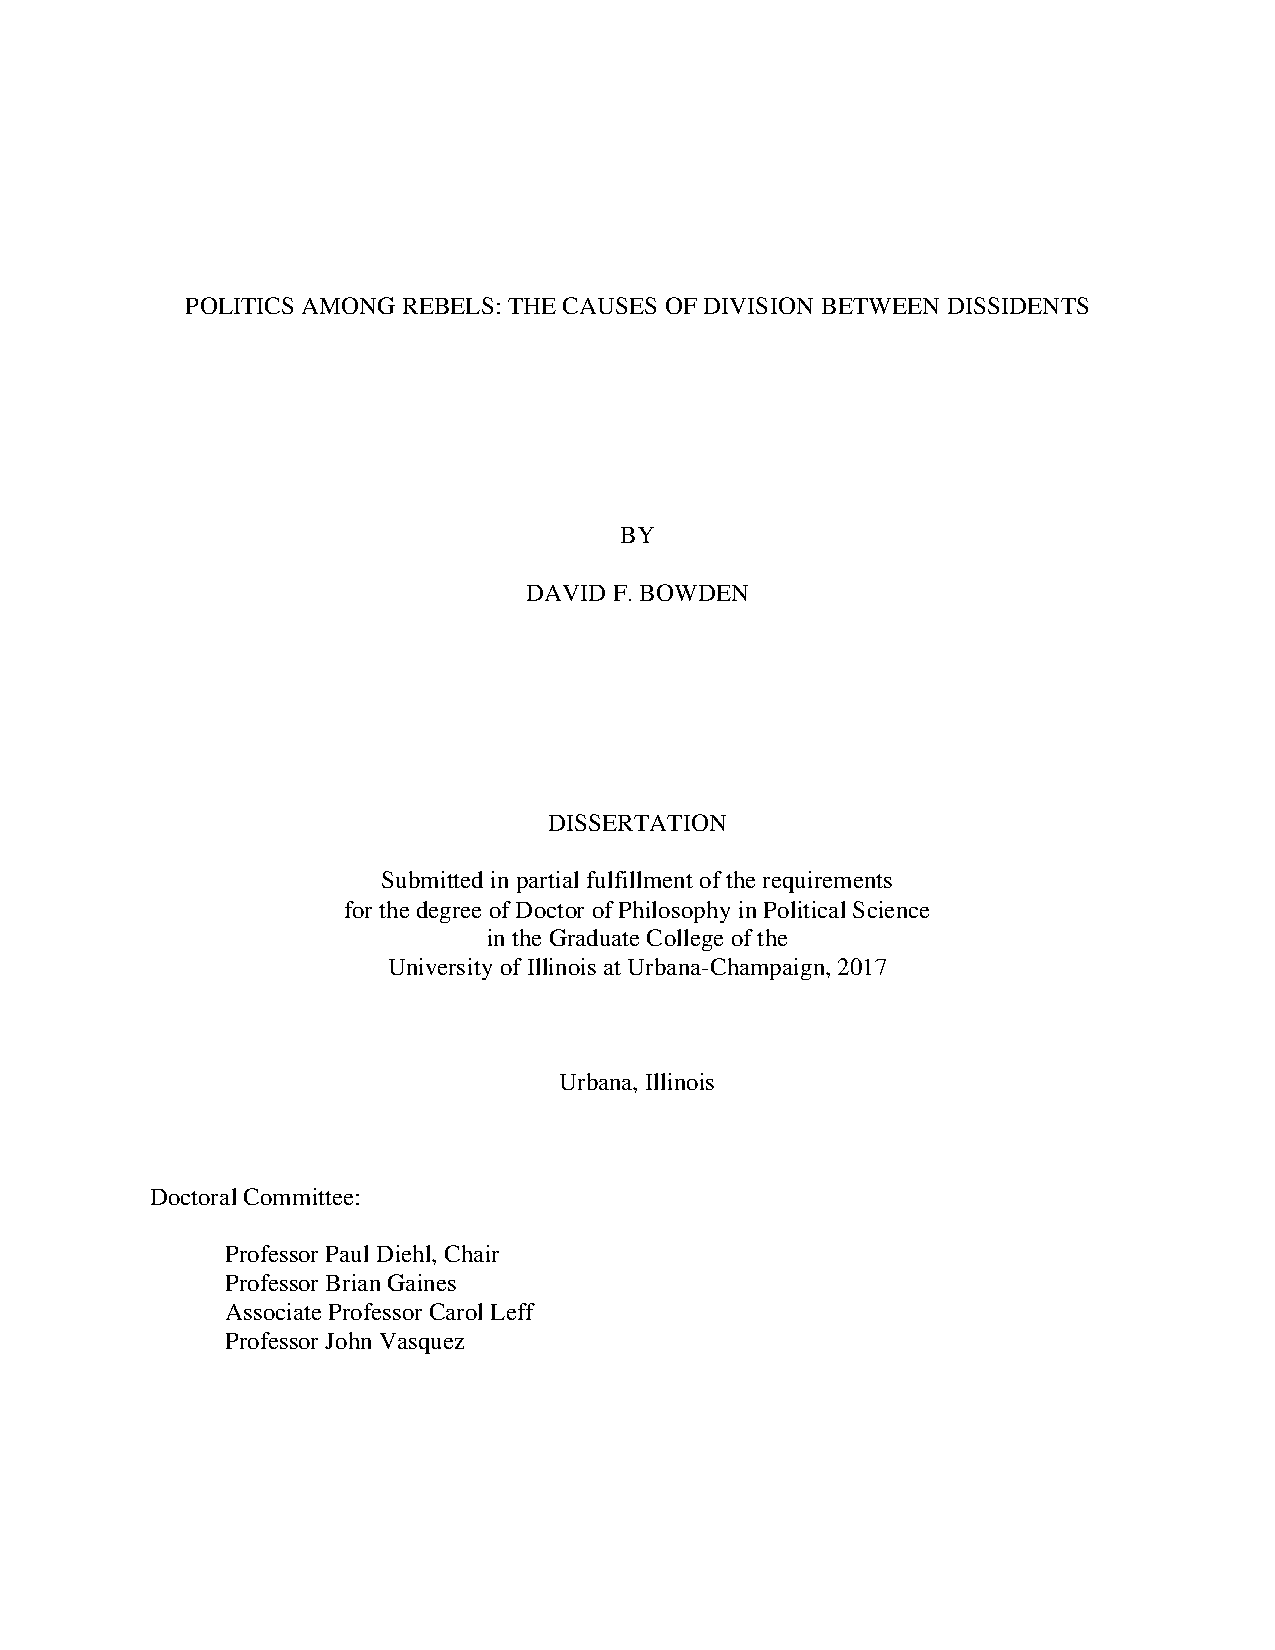
\includepdf[pages={1}]{titlepage.pdf}

\doublespacing

\pagenumbering{roman}

\hypertarget{abstract}{%
\chapter*{Abstract}\label{abstract}}

\setcounter{page}{2}

What explains the variation in the number of rebel groups across civil
conflicts? Prior research has established that conflicts with multiple
rebels groups are among the most severe cases in terms of duration,
fatalities, and possibilities for recurrence. Yet, we know little about
why the structure of rebel movements varies. This dissertation seeks to
resolve that gap. I argue that the organization of rebellion is
contingent on the identities and ideologies that are most salient at a
given moment. Organization around ethnic identity tends to produce
fragmented movements with multiple rebel groups. I expect that ethnicity
will tend to be salient when civilians are targeted with repression.
Three empirical analyses provide support for this contention. I show
that individuals who have been attacked are more willing to use violence
and more likely to identify with their ethnic group. Next I show that
repression significantly increases the probability that new rebel groups
will enter a conflict, and that these new groups are likelier than
others to emphasize a single ethnic identity. I also demonstrate that
repression triggers a reorganization of existing rebel groups around
ethnicity, with repression being associated with increased probabilities
of rebel group splintering and the formation of ethnically-homogeneous
alliances. I supplement these quantitative analyses with case studies of
several secessionist movements in Burma. Ultimately, I find that
repression substantially increases the probability that a conflict will
have multiple rebel groups.

% dedication
\pagebreak
\hspace{0pt}
\vfill
\begin{center}
\textit{For my family}
\end{center}
\vfill\hspace{0pt}
\pagebreak

% \hypertarget{acknowledgements}{%
% \chapter*{Acknowledgements}\label{acknowledgements}}

\begingroup
\renewcommand{\cleardoublepage}{}
\renewcommand{\clearpage}{}
\chapter*{Acknowledgements}
\endgroup

I am grateful to many people who have helped me through my academic journey. First, Paul Diehl has been a truly outstanding advisor. He has been an excellent teacher and mentor who dramatically improved my ability to think clearly about armed conflict, consistently pushed me to improve my work, and conferred on me a tremendous amount of knowledge about teaching, publishing, and countless other professional skills. His absurdly prompt feedback and advice were especially welcome in the past year as I completed this dissertation and navigated the job market.

The other members of my dissertation committee were invaluable as well. John Vasquez taught me a great deal about theorizing and thinking scientifically about international relations, and has been incredibly supportive throughout my time at Illinois. Brian Gaines brought much-needed methodological expertise and attention to detail to the committee. Carol Leff was a late addition to the committee, but provided many excellent insights regarding ethnic politics and the qualitative case studies. 

I also benefited from the teaching, advice, and support of numerous other faculty and staff members at Illinois. Bob Pahre served on the committee at the prospectus stage and consistently provided a unique and useful prospective on my work. Xinyuan Dai was enthusiastically supportive while I completed my coursework and exams, and Jim Kuklinski's research design class stands out as a highlight of that portion of my career. I began exploring an early version of the idea for this dissertation while a Schroeder Fellow at the Cline Center for Advanced Social Research. I am thus grateful to the Schroeder brothers for funding the position, and to Pete Nardulli and Scott Althaus for their valuable work at the Cline Center. Maryalice Wu provided me with a year of funding and the opportunity to refine my methodological skills at the Center for Innovation in Teaching and Learning. Finally, Brenda Stamm is surely one of the most talented and dedicated administrators at the University of Illinois, and I am grateful for all her help over the years in navigating departmental and university procedures.

I was extremely fortunate to go through the PhD program with a wonderful group of fellow students from whom I learned a great deal, and who also provided excellent companionship along the way. Watching basketball with Paul Testa and Kyle Estes was the best occasional distraction from political science anyone could ask for, and coffee klatch with Gina Reynolds, Tarah Williams, and a rotating cast of others was always a highlight of my week. There were many others with whom I greatly enjoyed spending time, including Kaye Usry, Jason Renn, Ashly Townsen, Bryce Reeder, Todd Robinson, Matt Powers, Tyler Pack, Blair Niece, Gina Martinez, Matt Spears, Bryce Dietrich, and Ashlea Rundlett. I have undoubtedly forgotten many more, and for that I apologize.

Lastly, none of this would have been possible without the support of my family. My parents, Ann and Bob, financed my undergraduate eduction. They and my grandmother, Alice Bowden, provided me with frequent financial help through my time as a graduate student. More importantly, they always regarded pursuing a PhD as a normal thing to do with one's life, and were incredibly encouraging every step of the way. Thank you all.

\singlespacing

{
\setcounter{tocdepth}{1}
\tableofcontents
}

\doublespacing

\mainmatter

\hypertarget{intro}{%
\chapter{Introduction}\label{intro}}

Why do some civil wars have multiple rebel groups, while others have
only one? Theories of civil war tend to focus on individual-level
motives (e.g. Gurr \protect\hyperlink{ref-gurr70}{1970}; Collier and
Hoeffler \protect\hyperlink{ref-Collier2004}{2004}) or opportunities
(e.g. Fearon and Laitin \protect\hyperlink{ref-fearonlaitin03}{2003})
for rebellion, while giving little attention to the organization of
dissent into rebel groups and coalitions. Even those studies which do
explicitly consider rebel group formation tend to focus on group
attributes such as their relationship with civilians (e.g. Weinstein
\protect\hyperlink{ref-Weinstein2007}{2007}), and do not consider the
structure of the rebel movement that emerges. Yet, the process of
organizing rebel groups is not always straightforward. At least two
rebel groups are simultaneously active at some point in 44\% of civil
conflicts.\footnote{Source: Pettersson and Wallensteen
  (\protect\hyperlink{ref-Pettersson2015a}{2015}).} In the Chadian Civil
War, for instance, 25 distinct rebel groups appeared over the course of
the conflict. Conflicts in Afghanistan in the 1980's, Somalia in the
1990's, and Sudan in the 2000's have been similarly complex. At its peak
the recent civil war in Syria was contested by at least two dozen armed
groups. Even movements with geographically-concentrated populations and
common goals, such as the Arakanese secessionists in Burma, often
fragment into multiple rebel groups. Furthermore, the number of groups
operating in these conflicts often varies greatly over time. Returning
to the Syrian example, the opposition was largely consolidated under the
banner of the Free Syrian Army early in the conflict, later splintered
into dozens of factions largely on the basis of religion, and now
appears to be consolidating again as groups are defeated or merge.

The importance of rebel movement\footnote{Throughout this dissertation,
  I use the term ``rebel movement'' to refer to the entire set of rebel
  groups.} structure has been well established, with several studies
examining the consequences of having multiple rebel groups. Generally,
these works find that the presence of multiple rebel groups is
associated with greater levels of conflict severity. Conflicts of this
type last longer than dyadic competitions, as the increased number of
veto players complicate the negotiation of peaceful settlements
(Cunningham \protect\hyperlink{ref-Cunningham2006}{2006}; Cunningham,
Gleditsch, and Salehyan \protect\hyperlink{ref-Cunningham2009}{2009};
Akcinaroglu \protect\hyperlink{ref-Akcinaroglu2012}{2012}), and create
the possibility of peace being spoiled by extreme factions (Stedman
\protect\hyperlink{ref-Stedman1997}{1997}). Relatedly, Cunningham,
Gleditsch, and Salehyan (\protect\hyperlink{ref-Cunningham2009}{2009})
find that the presence of multiple government-rebel dyads decreases the
likelihood that a conflict will end with a peace agreement, while
increasing the likelihood of rebel victory. Findley and Rudloff
(\protect\hyperlink{ref-Findley2012}{2012}) find this effect to be
conditional, however, as the fragmentation of weak rebel movements can
increase the probability of peaceful settlement. Perhaps related to the
paucity of peaceful settlements, both Atlas and Licklider
(\protect\hyperlink{ref-Atlas1999}{1999}) and Zeigler
(\protect\hyperlink{ref-Zeigler2016}{2016}) find that civil wars with
multiple rebel groups are prone to recurrence, as new episodes of
conflict frequently occur between rebel factions that were separate in
the previous conflict. Finally, conflicts with multiple dyads feature
over 20\% more fatalities than dyadic ones.\footnote{Source: my own
  analysis using data from Sundberg
  (\protect\hyperlink{ref-Sundberg2008a}{2008}).} In short, conflicts
with multiple rebel groups are an unusually severe subset of civil wars.

While prior research has firmly established the importance of
understanding why some conflicts have multiple rebel groups while others
do not, few existing works have attempted to explain this phenomenon.
The studies that do exist in this area tend to focus on a narrow subset
of the processes affecting conflict complexity. For example, several
recent works explore the splintering of existing rebel groups (e.g.
McLauchlin and Pearlman \protect\hyperlink{ref-McLauchlin2012}{2012};
Staniland \protect\hyperlink{ref-Staniland2014}{2014}). These studies
tend to focus on the internal characteristics of rebel groups however,
and thus have little to say about why rebel groups might form alliances,
nor why entirely new groups might enter a conflict. Christia
(\protect\hyperlink{ref-Christia2012}{2012}) adapts realism from
international relations theory into a joint explanation of splintering
and alliance formation, but she too ignores the mobilization of new
groups. I connect all three phenomena in a single theoretical framework,
providing a unified explanation for conflict complexity.

The goal of this project is to address a single broad research question:
what explains the variation in the number of rebel groups in a civil
war? I address several more specific questions in pursuit of this
broader goal. How do individuals respond to violence? Under what
conditions do new rebel groups join an ongoing civil war? Why do
existing rebel groups splinter into multiple factions? Why do previously
independent rebel groups form alliances?

In brief, I argue that the treatment of civilians during wartime is a
crucial determinant of rebel movement cohesion. Violent repression
should lead many civilians to calculate that joining a rebellion is not
dramatically riskier than remaining non-violent, increasing the pool of
individuals willing to fight. But as repression is often applied on the
basis of ethnicity, and ethnic groups often offer a useful basis for
organizing defensive measures and attracting external support,
repression should also tend to induce greater levels of ethnic
identification. Thus, repression should expand the pool of individuals
willing to join the fighting, but also sow division among dissidents
along ethnic lines. I expect that this dynamic will influence all three
processes identified in the existing literature as determinants of
conflict complexity --- the formation of new rebel groups, the
splintering of existing rebel groups, and the merger of previously
independent groups into alliances. The results of my empirical chapters
suggest that complex civil wars are often the result of a sectarian
spiral --- an initial wave of repression mobilizes violent dissent and
induces greater levels of ethnic identification, and the rebel movement
fragments along ethnic lines to reflect these individual-level
preferences. Prior work suggests that a more fragmented movement might
lead to greater levels of conflict severity, potentially creating a
vicious circle.

In the remainder of this chapter I review the existing literature on
rebel movement structure, as well as prior work on repression and ethnic
identification. Next, I summarize the broader theoretical and policy
implications of the research. Finally, I provide a summary of the
subsequent chapters.

\hypertarget{previous-work-on-the-organization-of-rebellion}{%
\section{Previous Work on the Organization of
Rebellion}\label{previous-work-on-the-organization-of-rebellion}}

The existing literature and empirical record suggest that the number of
rebel groups active in a conflict is shaped by three broad processes.
New groups can emerge when previously non-violent individuals mobilize
and join the conflict. Alternatively, previously cohesive rebel groups
can splinter into multiple successor organizations. Finally, the number
of rebel groups can decrease when previously independent factions form
alliances. I summarize the literature on each process in turn, and
relate my contributions to the existing work.

\hypertarget{group-formation}{%
\subsection{Group Formation}\label{group-formation}}

Around 30\% of conflicts have at least one rebel group that was neither
active from its beginning, nor did it split from an existing rebel
group. Thus, the formation of new rebel groups during ongoing conflicts
is an important determinant of rebel movement structure. Yet few studies
directly consider this phenomenon. Even studies of civil war onset often
leave the formation of rebel groups in a black box, instead making a
leap from individual motives to war initiation. For instance, a large
literature views rebellion as an essentially criminal activity, driven
by greed (Mueller \protect\hyperlink{ref-mueller00}{2000}; Collier and
Hoeffler \protect\hyperlink{ref-Collier2004}{2004}; Lujala, Gleditsch,
and Gilmore \protect\hyperlink{ref-Lujala2005}{2005}). Yet these works
generally have very little to say about the origins of rebel
organizations. These groups could be pre-existing criminal organizations
that initiate more violent activity in hopes of securing greater profit,
they could form for the purpose of a greed-driven rebellion after a sign
of weakness from the government, or they could begin as rebel groups
with sincere political goals, which are later seduced into less noble
pursuits. The grievance school similarly tends to neglect group
formation. For example, Cederman, Wimmer, and Min
(\protect\hyperlink{ref-Cederman2010}{2010}) offer a nuanced explanation
of the conditions under which ethnic minorities are likely to rebel.
Yet, they say little about the logistics of organizing a rebellion, and
seemingly assume that ethnic groups have an inherent ability to spawn
rebel organizations.

Scholars working at lower levels of analysis have come closer to
explaining group formation. Kalyvas
(\protect\hyperlink{ref-Kalyvas2006}{2006}) suggests that individuals
are often already mobilized for small-scale violence such as personal
rivalry, criminal activity, or ethnic conflict. Building a rebel group
is thus an exercise in building coalitions from small, pre-existing
organizations, and re-orienting individuals from localized issues to
national-level political cleavages. Kalyvas gives little attention to
this process in his empirical analyses, however, instead recommending it
as an area for future research. Staniland
(\protect\hyperlink{ref-Staniland2014}{2014}) also argues that most
rebel groups can trace their origins to pre-existing social
organizations, though he sees larger, and often more political entities
such as political parties or military units as the primary source of
rebellion, rather than the localized and less formal groups emphasized
by Kalyvas (\protect\hyperlink{ref-Kalyvas2006}{2006}). Staniland
(\protect\hyperlink{ref-Staniland2014}{2014}) focuses primarily on
linking the attributes of the originating organizations to rebel group
outcomes such as durability, however, and does not give much
consideration to the initial formation of these groups. Lewis
(\protect\hyperlink{ref-Lewis2016}{2016}) provides one of the few
studies that does explicitly consider rebel group formation, as she
carefully documents the earliest activities of rebel groups in Uganda.
She finds that rebel groups, including the Lord's Resistance Army, were
typically founded by small number of entrepreneurial individuals, and
initially tended to value stealth over broad mobilization. Only after
the conflict began to escalate did groups seek to broaden their
membership, in many cases by appealing to particular ethnic groups. Thus
she sees scholars such as Cederman, Wimmer, and Min
(\protect\hyperlink{ref-Cederman2010}{2010}) and Staniland
(\protect\hyperlink{ref-Staniland2014}{2014}) as beginning their
analyses after rebellion had existed for some time.

Also of relevance to group formation is the substantial literature on
the contagion of civil war. Gleditsch
(\protect\hyperlink{ref-Gleditsch2007}{2007}) finds that transnational
ethnic groups and political and economic linkages between states can
provide channels for civil war to spread across international
boundaries. Most of his cases, however, are pre-existing rebel groups
moving into new geographic areas, rather than instances of \emph{sui
generis} group formation. Other scholars find that entirely new rebel
organizations can emerge through the contagion of secessionist (Ayres
and Saideman \protect\hyperlink{ref-Ayres2000}{2000}) and ethnic (Lane
\protect\hyperlink{ref-Lane2016}{2016}) conflict. Such transnational
processes might shape opportunities for multiple rebellions to emerge by
increasing the availability of weapons, spreading tactical knowledge, or
diverting government attention to foreign conflicts. While contagion
explains an important category of phenomena, these studies are primarily
concerned with the spread of conflict to previously peaceful areas, and
do not necessarily explain the phenomenon of new groups joining ongoing
conflicts.

\hypertarget{splintering}{%
\subsection{Splintering}\label{splintering}}

Another process affecting rebel movement structure is the splintering of
existing organizations. In 1968, for example, a faction led by Ahmed
Jibril broke away from the Popular Front for the Liberation of Palestine
(PFLP) to form a new group, the Popular Front for the Liberation of
Palestine-General Command (PFLP-GC). While the two groups have often
collaborated against Israel, they maintain distinct organizational
structures and membership bases, and operate in different areas. The
split was allegedly motivated by differing views of Marxist ideology and
military doctrine, with the PFLP pursuing a more extreme strategy of
attrition. Similar splits have occurred within dozens of rebel groups,
including the Communist Party of Burma, the Free Syrian Army and the
Sudan Liberation Army. In many cases the result is more than a nominal
separation. In Sri Lanka, for example, the Tamil Peoples Liberation
Tigers not only split from the Liberation Tigers of Tamil Eelam, but
also defected to the government's side in the conflict (Staniland
\protect\hyperlink{ref-Staniland2012d}{2012}).

Compared to group formation, there is a relatively large literature on
rebel group splintering. One subset of this research focuses on the role
of external actors, and particularly the government. For instance,
McLauchlin and Pearlman (\protect\hyperlink{ref-McLauchlin2012}{2012})
find that government repression provides occasion for groups to evaluate
their current leadership structure. Pre-existing divisions within groups
are likely to be exacerbated, leading the group to move toward more
factionalized leadership structures. When group members are satisfied,
however, conflict tends to lead to even greater unity and centralization
of authority. Whereas the preceding studies essentially treat government
repression as exogenous to the internal politics of dissident groups,
Bhavnani, Miodownik, and Choi
(\protect\hyperlink{ref-Bhavnani2011}{2011}) present evidence that
governments deliberately stoke tensions among their opponents, as they
find that the Israeli government increased conflict between Fatah and
Hamas by undermining Hamas' control of the Gaza and by tolerating
Fatah's relationship with the Jordanian military. Relatedly, Tamm
(\protect\hyperlink{ref-Tamm2016}{2016}) finds that support from outside
states can alter the balance of power within rebel groups, in some cases
entrenching existing hierarchies, while in others creating possibilities
for fragmentation or coups. Finally, Staniland
(\protect\hyperlink{ref-Staniland2012d}{2012}) finds that the government
can sometimes attract rebel groups to their side by offering greater
resources during periods of infighting among rebel groups.

Another group of scholars emphasizes concerns about post-conflict
bargaining as the key determinant of dissident group cohesion. Christia
(\protect\hyperlink{ref-Christia2012}{2012}) assumes that the winning
coalition in a civil war receives private benefits, which might include
any rents available to the state, and having some portion of its
interests represented in the new government. Thus, rebels have an
incentive to form minimum winning coalitions, so as to limit the number
of coalition partners with whom they must share benefits. Wolford,
Cunningham, and Reed (\protect\hyperlink{ref-Wolford}{2015}) develop a
similar logic, theorizing that political factions have an interest in
joining conflicts in hopes of maximizing the likelihood that their
preferences will be represented in the post-war government. The value of
fighting decreases, however, as the number of parties with whom they
expect to share power increases. Yet, Christia
(\protect\hyperlink{ref-Christia2012}{2012}) suggests that this
incentive to minimize coalition size is moderated by the risk of being
outside the winning coalition, as there is a strong possibility of new
waves of violence between victorious rebels and rival rebel factions.
She thus expects coalitions to change frequently in response to
battlefield events, with factions bandwagoning with battle winners and
shifting away from losing coalitions. Findley and Rudloff
(\protect\hyperlink{ref-Findley2012}{2012}) similarly find fragmentation
to be most common among groups that have recently lost battles. This
implies that fragmentation is essentially a process of weak actors
becoming weaker.

A final category of explanations places the source of rebel group
cohesion in underlying social structure. Staniland
(\protect\hyperlink{ref-Staniland2014}{2014}) argues that insurgent
organizations will be most stable when their central leadership is able
to exercise both vertical control over its rank-and-file members, and
horizontal control over its constituent groups. This is most likely to
occur when insurgencies draw from existing organizations with extant
social ties of this sort, which might include former anti-colonial
movements or ethnic political parties. Organizations are likely to
fragment when constituent groups have a high degree of autonomy or
control over individual members is limited (Staniland
\protect\hyperlink{ref-Staniland2014}{2014}, Ch. 2-3). Asal, Brown, and
Dalton (\protect\hyperlink{ref-Asal2012}{2012}) emphasize similar
factors, arguing that organizations with factionalized leadership
structures are at risk of fragmentation, while groups with more
consolidated power structures will tend to remain cohesive. Finally,
Warren and Troy (\protect\hyperlink{ref-Warren2015}{2015}) suggest that
group size plays an important role, as small groups are able to police
themselves and resolve conflicts, whereas larger groups are more likely
to experience infighting.

\hypertarget{alliance-formation}{%
\subsection{Alliance Formation}\label{alliance-formation}}

Whereas the formation of new groups and splintering can increase the
complexity of a civil war, the number of rebel groups can also be
reduced through the formation of alliances. Many of the most successful
rebel movements in history were coalitions of formerly independent
organizations. For example, the Frente Farabundo Marti para la
Liberacion Nacional (FMLN) was an umbrella organization uniting several
left wing rebel groups in El Salvador, which eventually secured many
concessions in the post-war peace process including a place as a major
political party. Surprisingly, however, alliances among non-state actors
have only recently begun to receive much scholarly attention.

Asal and Rethemeyer (\protect\hyperlink{ref-Asal2008}{2008}) and
Horowitz and Potter (\protect\hyperlink{ref-Horowitz2013}{2013}) conduct
network analyses of alliance formation among terrorist groups, arguing
that such arrangement are used to aggregate capabilities and share
tactics. Much of the other work in the field focuses on the downsides of
alliance. Bapat and Bond (\protect\hyperlink{ref-Bapat2012}{2012})
assume that alliances carry two significant costs: the dilution of each
constituent group's agenda, and the risk of having one's private
information sold to the government by an ally. Consistent with this
theory, they find alliances to be most common when an outside state can
enforce agreements, and when all rebel groups involved are strong enough
to avoid the temptation of defecting to the government side. Christia
(\protect\hyperlink{ref-Christia2012}{2012}) similarly emphasizes
capability, arguing that neorealist balancing theory from international
relations explains alignments in civil wars. When one coalition - a
group of rebels or government-aligned forces - becomes too powerful,
other groups will band together to prevent their own destruction. But
similar to Bapat and Bond (\protect\hyperlink{ref-Bapat2012}{2012}),
Christia (\protect\hyperlink{ref-Christia2012}{2012}) argues that this
mechanism is constrained by a desire to maximize one's share of the
post-war spoils. Thus, rebels should realign frequently, seeking to form
minimum winning coalitions. While shared identity appears on the surface
to be an important determinant of rebel alignments, Christia views these
narratives as post-hoc justifications aimed at legitimizing decisions
that are really driven mostly by power.

\hypertarget{repression}{%
\subsection{Repression}\label{repression}}

As repression is central to the theoretical argument presented here,
this dissertation is shaped by the literature on the topic. The focus in
the existing work has been on explaining why repression occurs, and
identifying factors that might prevent it. Davenport
(\protect\hyperlink{ref-Davenport2007a}{2007}\protect\hyperlink{ref-Davenport2007a}{b})
finds that there is a ``domestic democratic peace,'' meaning that
democratic regimes tend to refrain from using the most violent forms of
repression. However, he finds that even democracies often engage in
repression during civil and international conflicts. Others find that
international human rights treaties often have a meaningful restraining
effect on governments, reducing their use of repression (Hathaway
\protect\hyperlink{ref-Hathaway2002}{2002}; Simmons
\protect\hyperlink{ref-simmons09}{2009}). Not all international
influences are positive, however, as economic sanctions (Wood
\protect\hyperlink{ref-Wood2008a}{2008}) are associated with increased
repression. An important generalization in the context of this study is
that human rights practices tend to be shaped by domestic and
international political institutions that are likely to be largely
exogenous to civil war dynamics.\footnote{Long-running civil wars,
  however, might deter democratization and participation in human rights
  treaties.} Another strand of the repression literature focuses on the
consequences of repression, and especially the potential of repression
to provoke escalation. In this vein Lichbach
(\protect\hyperlink{ref-Lichbach1987}{1987}) argues that repression
should lead dissidents to substitute increasingly violent tactics for
more peaceful ones, as they will calculate that violence is more likely
to achieve their goals. Moore (\protect\hyperlink{ref-Moore1998}{1998})
finds empirical support for this model, suggesting that repression has
significant potential to escalate political confrontations.

\hypertarget{ethnic-identification}{%
\subsection{Ethnic Identification}\label{ethnic-identification}}

Ethnic identity is central to the theoretical mechanism in this
dissertation, and has long been an area of deep interest to scholars of
comparative politics. This work is often predicated on the assumption
that identity is dynamic. At a minimum, individuals can choose which of
their several social roles to emphasize. For instance, individuals might
orient primarily toward an ethnicity, a religion, an occupation, a
region, or an ideology, and could potentially alter these choices over
time. The majority of the work in this vein has focused on oscillations
between ethnic and national identities. Early on this question was
explored in the context of statebuilding. Scholars in this area suggest
that external threats such as interstate wars (Herbst
\protect\hyperlink{ref-Herbst1990}{1990}; Tilly
\protect\hyperlink{ref-Tilly1992}{1992}) or territorial disputes
(Gibler, Hutchison, and Miller \protect\hyperlink{ref-Gibler2012}{2012})
can provide a unifying influence, leading individuals to orient toward
national identities and away from subnational ones such as ethnicity.
Most other work in the area examines the role of political institutions
in incentivizing the use of particular identities (Posner
\protect\hyperlink{ref-Posner2005}{2005}; Penn
\protect\hyperlink{ref-Penn2008}{2008}). For example, Eifert, Miguel,
and Posner (\protect\hyperlink{ref-Eifert2010}{2010}) find that ethnic
identification tends to be strongest just prior to or just after
competitive elections, suggesting that individuals interpret politics
through an ethnic lens.

A striking feature of this literature is the degree of consensus that
ethnic identity is malleable. This perspective is shared by a diverse
range of scholars ranging from constructivists (e.g. Barnett
\protect\hyperlink{ref-Barnett1995}{1995}) to formal theorists (e.g.
Penn \protect\hyperlink{ref-Penn2008}{2008}), and enjoys strong
empirical support (e.g. Eifert, Miguel, and Posner
\protect\hyperlink{ref-Eifert2010}{2010}; Gibler, Hutchison, and Miller
\protect\hyperlink{ref-Gibler2012}{2012}). Notably, recent work has
shown that repression is an important factor in shaping identity, with
effects that persist not only over long periods of time, but across
generations as well. Lupu and Peisakhin
(\protect\hyperlink{ref-Lupu2017a}{2017}) show that the descendants of
Crimean Tatars who were deported by Soviet forces 1940's are more
supportive of Tatar political leaders, have greater antipathy towards
Russia, and are more likely to participate in politics as compared to
Tatars with no such family history. Relatedly, Rozenas, Schutte, and
Zhukov (\protect\hyperlink{ref-Rozenas2017}{2017}) show that Ukrainian
communities that were subjected to greater levels of deportation during
this period are today less supportive of pro-Russian political parties
than are comparable communities that experienced less deportation. In
short, the malleability approach provides a strong foundation on which
to build my theory.

\hypertarget{rebel-motives}{%
\subsection{Rebel Motives}\label{rebel-motives}}

An examination of the relationships between dissident groups is also
likely to offer a new perspective on rebel motives. The literature on
civil war has largely been dominated by debates over whether rebellion
is fundamentally political, or done in pursuit of private benefits. The
former views civil war as an effort to resolve economic or political
inequality (Gurr \protect\hyperlink{ref-gurr70}{1970}; Wood
\protect\hyperlink{ref-Wood2003}{2003}; Cederman, Wimmer, and Min
\protect\hyperlink{ref-Cederman2010}{2010}), and has been labeled as the
`grievance' hypothesis (Collier and Hoeffler
\protect\hyperlink{ref-Collier2004}{2004}). The latter is composed
primarily of studies emphasizing the `greed' hypothesis (Collier and
Hoeffler \protect\hyperlink{ref-Collier2004}{2004}), which views
rebellion as little more than large-scale criminal activity aimed at
bringing profits to its members (Mueller
\protect\hyperlink{ref-mueller00}{2000}; Lujala, Gleditsch, and Gilmore
\protect\hyperlink{ref-Lujala2005}{2005}; Ross
\protect\hyperlink{ref-Ross2004e}{2004}). Others have emphasized
non-material private benefits as motive for individual participation in
rebellion, such as the ability to act on family disputes or romantic
rivalries (Kalyvas \protect\hyperlink{ref-Kalyvas2006}{2006}).

This political-private motive debate has yet to be definitively
resolved. A number of scholars have found greater support for the greed
hypothesis than for grievance, with the presence of natural resources
being a stronger predictor of civil war than economic or political
grievances (Collier and Hoeffler
\protect\hyperlink{ref-Collier2004}{2004}). Yet, these findings are not
robust across different types of resources or even different measures of
the same resource (Dixon \protect\hyperlink{ref-Dixon2009a}{2009}).
Furthermore, several scholars have found that political factors such as
hierarchical relationships between ethnic groups (Cederman, Wimmer, and
Min \protect\hyperlink{ref-Cederman2010}{2010}) and poor economic
performance (Miguel, Satyanath, and Sergenti
\protect\hyperlink{ref-Miguel2004a}{2004}) exert a strong influence on
civil war onset. Other scholars eschew the dichotomy altogether,
suggesting that while private benefits are useful to rebel recruiting
efforts, this does not preclude the possibility that rebel elites
ultimately have political motives (Lichbach
\protect\hyperlink{ref-Lichbach1995}{1995}; Weinstein
\protect\hyperlink{ref-Weinstein2007}{2007}). Similarly, Lujala
(\protect\hyperlink{ref-Lujala2010}{2010}) finds that natural resources
are associated with longer conflicts, implying that at least a portion
of resource revenues are devoted to fighting rather than private
benefits.

One factor that has limited progress on these questions of motive is the
fact that the competing theories have been tested almost exclusively on
a single outcome --- a binary measure of the occurrence of civil war at
the national level. Studying the relationships between dissident groups
and how they vary is likely to provide insight to underlying rebel
motives. For instance, if rebellion is fundamentally about maximizing
the profits of its members, we might expect to see rebels form the
smallest coalitions possible that still allow them to control resource
flows. If rebellion is fundamentally political, however, we might expect
rebels to pursue coalitions large enough to pursue victory.
Additionally, if ideology and identity are not truly important to
rebels, splintering and alliance formation should be driven primarily by
power calculations (see Christia
\protect\hyperlink{ref-Christia2012}{2012}). If these factors do matter,
however, they should shape the choice of alliance partners and the
cohesiveness of individual groups. Ethnically homogeneous rebel groups
should be less prone to splintering in this case, and alliance should be
more likely among groups with similar identities.

\hypertarget{the-contribution-of-this-project}{%
\section{The Contribution of this
Project}\label{the-contribution-of-this-project}}

First and foremost, this project advances our understanding of a subset
of civil wars that is crucially important for the reasons outlined
above. This research explains three processes that account for most of
the variation in the number of rebel groups in a conflict --- the entry
of new groups, and the splintering and mergers of existing ones. This
dissertation is among the first projects to directly address the first
phenomenon of new rebel groups joining ongoing conflicts. Existing work
either considers the formation of new rebel groups (i.e.~groups that
were not previously contained within another violent organization) only
in cases where it is coterminous with conflict initiation (e.g. Lewis
\protect\hyperlink{ref-Lewis2016}{2016}), or in the context of contagion
into previously peaceful areas (e.g. Lane
\protect\hyperlink{ref-Lane2016}{2016}). Yet, I find that 27.5\% of
rebel groups active since World War II were neither present from the
beginning of the conflict, nor is there any evidence that they descended
from existing rebel groups. An important contribution of this
dissertation, then, is explaining this common but mostly ignored
phenomenon.

While splintering and alliance formation have been the subject of
several prior studies, my findings largely contrast with existing work.
Christia (\protect\hyperlink{ref-Christia2012}{2012}) argues that
realist power politics calculations drive both alliance formation and
splintering. Asal, Brown, and Dalton
(\protect\hyperlink{ref-Asal2012}{2012}) and Staniland
(\protect\hyperlink{ref-Staniland2014}{2014}) suggest that
organizational structure is the key determinant of rebel cohesiveness. I
find no evidence for this, however, as rebel group centralization is not
related to splintering in my analyses. Furthermore, my argument offers
much clearer predictions than existing work regarding the timing of
splintering and alliance formation, and regarding the choice of alliance
partners. Additionally, the existing research is largely based on a
small number of case studies disproportionately drawn from the Middle
East and South Asia. While these conflicts are undeniably complex, they
are outliers in terms of both their long duration and high degree of
international intervention. I test my theory on a sample of all civil
wars since 1946, demonstrating that it is widely applicable.

I also build upon the existing literature by unifying explanations of
group formation, splintering and alliances into a more comprehensive
theory of rebel movement structure. I argue that all three processes
reflect the level of ethnic identification by dissidents, with
repression driving changes to this trait. Connecting these phenomenon
under a single framework provides a clear delineation of the
similarities and differences in the processes through which each type of
group emerges. Either implicitly through its treatment of them as
distinct phenomena, or explicitly through its theoretical arguments,
previous work suggests that these phenomena are largely unrelated.
Considering these processes jointly also allows me to make predictions
regarding the overall number of rebel groups active in a conflict, as I
do in Chapter \ref{realignment}.

My findings also suggest several important second-order implications.
One is that rebellion seems to be more political and more responsive to
the preferences of rank-and-file dissidents than much of the existing
literature would suggest. A substantial number of scholars view civil
war as largely apolitical, instead being driven by material greed
(Mueller \protect\hyperlink{ref-mueller00}{2000}; Collier and Hoeffler
\protect\hyperlink{ref-Collier2004}{2004}) or personal animosities
(Kalyvas \protect\hyperlink{ref-Kalyvas2006}{2006}). I argue that
dissidents have strong preferences over the content of rebellion, and
find that repression tends to induce stronger preferences for rebel
groups that represent the interests of a particular ethnic group. While
I cannot rule out the possibility that rebellions are initially driven
by material considerations, as war initiation is beyond the scope of
this study, my findings do suggest that civil war violence tends to have
a politicizing effect over time. I discuss the literature on rebel
motives in greater detail later in this chapter.

This work also suggests that governments can exert a powerful influence
on the structure of dissident organizations, as repression can heighten
the salience of identities that divide dissidents. This contrasts with
the most existing accounts of rebel movement structure, which tend to
focus on factors mostly internal to the rebel movement such as relative
power among rebel factions (Christia
\protect\hyperlink{ref-Christia2012}{2012}), or the strength of pre-war
social ties among dissidents (Staniland
\protect\hyperlink{ref-Staniland2014}{2014}). It also raises several
interesting questions about government strategy in the face of dissent.
My findings suggest that repression expands the pool of individuals
willing to fight, which in a vacuum makes government repression
puzzling. It is also unclear whether the other key consequence of
repression I identify --- the increased salience of ethnic identity ---
is a desirable outcome for the government. On one hand it could form the
basis of an effective divide-and-conquer strategy. On the other hand,
fighting multiple opponents could complicate the logistics of
counterinsurgency, threaten the credibility of negotiated settlements,
and undermine the prospects of a stable resolution to the conflict.
While this calculation merits greater consideration that I am able to
give it in this dissertation, my findings in Chapter
\ref{survey-chapter} suggest that repression may be aimed at deterring
dissidents from political activities other than rebellion, such as
voting.

To test my hypotheses, I collected data on the origins of rebel groups.
This allows me to distinguish between groups that splintered from
existing rebel groups, groups engaging in violence for the first time,
and coalitions of previously active groups. I suspect that the causal
factors behind the emergence of each of these types are related, but as
the processes are quite distinct they should be studied separately.
Though I do not make much of the distinctions in this project, the data
also distinguish between several categories of groups that were not
previously engaged in rebellion, including political organizations,
religious organizations, apolitical militias, and factions of the regime
military. These categories should be useful for a variety of future
studies on topics such as the durability of rebel groups, their
probability of victory, and their treatment of civilians.

In addition to resolving a gap in the scholarly literature, a better
understanding of rebel movement structure is of value to policymakers.
As noted above, conflicts with multiple rebel groups are among the most
severe. Simply being able to predict which conflicts are likely to
become severe through this mechanism has several useful applications.
Policymakers might be able to identify early on the conflicts that are
most likely to benefit from peace operations. Humanitarian organizations
could predict which conflicts are likely to produce large numbers of
refugees, and distribute resources accordingly. This work also be the
possibility of moving beyond prediction and solving the underlying
problem. As the empirical analyses identify the repression of civilians
as a key mechanism driving conflict complexity, it stands to reason that
protecting civilians might be an especially valuable undertaking for
non-governmental organizations or outside states.

In the next section I situate my dissertation in the literature to which
it is most closely related. I explain in greater detail my contributions
over the existing work on rebel structure, and also discuss the
implications of this work for the literatures on repression and ethnic
identification.

\hypertarget{project-summary}{%
\section{Project Summary}\label{project-summary}}

In Chapter \ref{theory} I articulate a theory of rebel movement
structure. I begin with the assumption that rebel groups emerge from a
broader pool of dissidents. While not all dissidents will be eager to
participate in violence, each will prefer to be represented by a rebel
group which advances their political interests and provides them with
security. Thus, dissidents form a constituency that constantly evaluates
the performance of rebel groups, and will consider switching their
allegiance to new groups if the existing ones are lacking. In hopes of
seizing on this dynamic, rebel entrepreneurs will look for opportunities
to mobilize new groups by appealing to underrepresented identities and
ideologies. These appeals should be especially effective in the wake of
repression for two reasons. First, repression lowers the risk of
fighting relative to remaining peaceful, leading new individuals to join
the fighting. Second, as repression should induce greater levels of
ethnic identification. Repression is often targeted on the basis of
ethnicity, increasing its salience, and appeals for support from
outside, co-ethnic states might be especially effective in the presence
of human rights concerns. Thus repression not only creates a new pool of
individuals willing to fight, it also stokes division among dissidents
along ethnic lines. This should often lead individuals joining the
fighting to form new groups rather than join existing ones, and
individuals already in rebel groups to realign into more ethnically
homogeneous configurations. This should manifest in the form of both the
splintering of existing groups, particularly when existing groups are
multi-ethnic, and the formation of ethnically-homogeneous alliances so
as to replace the loss in capabilities due to fragmentation and
streamline access to support from co-ethnic outside states.

Chapter \ref{survey-chapter} tests the individual-level assumptions of
the theory. Using a sample of over 150,000 Afrobarometer Survey
responses, I find support for both of my key predictions regarding the
effects of repression. Individuals who have experienced an attack in the
past year are 30\% more likely than others to express willingness to use
violence themselves. Additionally, I find these individuals are 62\%
more likely to identify with their ethnic group than respondents who
have not experienced an attack. While I am unable to completely rule out
the possibility of reverse causality, the results hold after performing
coarsened exact matching, showing that attacked individuals do not
systematically differ from others on observable traits. These results
suggest that my theory performs as expected at the individual level.

Chapter \ref{entry} contains tests of my predictions regarding the
formation of new rebel groups during ongoing conflicts. I add my measure
of rebel group origin to the Uppsala Armed Conflict Dataset, resulting
in a sample of all civil wars, 1946--2015. I find that the probability
of a new rebel group joining an ongoing conflict during a given year has
a strong, negative relationship with changes in respect for human
rights. The largest observed increases in repression are associated with
more than a 60\% chance of new rebel groups forming, while the
probability is around 3\% in years with no substantial change in human
rights practices, and approaches zero in following improvements to human
rights. Contrary to my expectations, I find no evidence that ethnic
diversity places a scope condition on my theory; new rebel groups form
in a variety of societies. I also do not find evidence that rebels
groups which join ongoing conflicts are more likely than others to draw
their support from a single ethnic group. However, this result seems to
be driven by a large number of rebel groups with no discernible ties to
an ethnic constituency, and I do find that these joining rebel are
significantly less likely than others to be multi-ethnic coalitions. To
supplement these quantitative analyses, I illustrate the causal logic of
my theory in a qualitative case study of the emergence of the Shan State
secessionist movement in Burma, and use the Arakan separatist movement
in that country to identify nuances missing from my argument.

In Chapter \ref{realignment} I explore two processes through which
rebels reorganize --- splintering from existing groups, and the
formation of alliances. I find that increases in repression are
associated with an increased probability of rebel group splintering,
though the result is not entirely robust. I do not find evidence to
support my hypothesis that rebel groups which draw support from multiple
ethnic groups are more prone to fragmentation. This seems to largely
reflect the fact that ethnically-homogeneous groups are
disproportionately likely to fight long-lasting, low-intensity
separatist conflicts. Consistent with my expectations I find evidence
that repression increases the probability that new
ethnically-homogeneous alliances will form, while having no effect on
the formation multi-ethnic alliances. Though less robust than the
findings in previous chapters, these results suggest that repression can
initiate a process of realignment whereby rebels tend to leave
multi-ethnic coalitions and form new alliances centered around a
particular ethnic identity. I close the chapter with an analysis of the
total number of rebel groups in a conflict, and show that in the
aggregate repression greatly increases the probability that a
conflict-year will have multiple rebel groups.

Finally, I summarize the results in Chapter \ref{conclusion}, discuss
their theoretical and policy significance, and propose several avenues
for future research on this topic.

\hypertarget{theory}{%
\chapter{A Theory of Rebel Movement Structure}\label{theory}}

Why are civil conflicts sometimes contested by multiple rebel factions,
while in other cases by a single, cohesive group? At a given point in
time, I argue that it is the choice of ideologies and identities around
which rebellions mobilize that determines whether they incorporate most
of the dissidents in a society, or whether many dissidents are left to
form their own groups. These arrangements are often fragile, however, as
factors such as government repression can lead dissidents to become more
receptive to new bases of organization. Drawing on the literature
reviewed in Chapter 1, I identify three processes through which these
individual dynamics shape the number of rebel groups in a civil war.
First, entirely new groups can enter the conflict. Second, previously
cohesive groups can splinter into multiple successor organizations.
Finally, previously independent groups sometimes merge. In the remainder
of this chapter I articulate a set of assumptions, a theory of the
internal politics of dissident movements, and a set of hypotheses to be
tested in subsequent chapters.

\hypertarget{theoretical-framework}{%
\section{Theoretical Framework}\label{theoretical-framework}}

I begin by laying out my assumptions about the relevant actors in a
civil war, their interests, and the structure of their interactions.

\hypertarget{the-dissident-pool}{%
\subsection{The Dissident Pool}\label{the-dissident-pool}}

I start from the assumption that rebel groups are drawn from a broader
pool of dissidents. By dissident, I simply mean an individual who
opposes the government. Dissidents are grouped into a variety of
potentially overlapping organizations. Some may belong to non-violent
political organizations such as trade unions or political parties.
Others may use violence as members of a rebel group. Hereafter I ``rebel
movement'' as a term that encompasses all rebel groups, but excludes
non-violent dissidents. In some cases this rebel movement will consist
of a single group, if there is only one rebel organization associated
with the dissident pool. In the American Civil War, for example, the
dissidents were represented by a single Confederate Army, though even in
this case there were several militias with only a loose attachment to
the main rebel group. In other cases the rebel movement may contain
several distinct rebel groups, such as the Shan State conflict in Burma,
which has produced at least six rebel groups.

At the individual level, dissidents are likely to vary on several
dimensions. First, individuals differ in their level of involvement in
violence. Lichbach (\protect\hyperlink{ref-Lichbach1995}{1995}, 17)
identifies five gradations of participation which range from being
constituents who may not even consent to being represented by the
dissident movement, to activists who engage in political activity but
not necessarily violence, to militants who participate in violence or
work in close support of such efforts. For instance, civilian activists
may provide crucial material and logistical support to rebels (see
Weinstein \protect\hyperlink{ref-Weinstein2007}{2007}; Parkinson
\protect\hyperlink{ref-Parkinson2013c}{2013}). Relatedly, dissidents may
utilize different ``repertoires of contention'' (Tilly
\protect\hyperlink{ref-Tilly1986}{1986},
\protect\hyperlink{ref-Tilly2006}{2006}), perhaps reflecting the
resources and past behavior of the groups through which they are
mobilized. For example, some elements of the dissident pool might
specialize in non-violent actions such as boycott, others on
conventional political channels such as elections, while others in
engage in violence. In addition to varying across individuals, the
willingness to use violence is often dynamic --- previously violent
individuals often desert their rebel group, and previously non-violent
individuals can be moved to participate in the fighting.

Social identities form a second dimension of variation among dissidents.
A few dissident movements are exceptionally homogenous. For example,
some separatist movements benefit from a coincidence of ethnicity,
language, religion, and geographic location. In most cases, however,
there is some amount of diversity along these attributes. For example,
the Kurds share a common ethnicity and language, but practice a variety
of faiths. Bids to overthrow the central government might be made by
coalitions featuring representatives of multiple ethnic groups,
religions, languages, and regions. Rebel leaders often emphasize broad,
inclusive goals and identities, hoping to gain the support of a large
portion of society. Such coalitions are often vulnerable to ``outbidding
appeals'' (Rabushka and Shepsle
\protect\hyperlink{ref-Rabushka1972}{1972}; Horowitz
\protect\hyperlink{ref-horowitz85}{1985}), through which moderate,
diverse groups lose support to competitors claiming to explicitly
represent a particular identity group.

Finally, while dissidents share a common interest in removing the
incumbent government, they do not necessarily agree on many other
political questions. Rural dissidents might make land reform their top
priority in a post-war government, whereas urban dissidents might care
more about corruption or modernization programs. Some dissidents hope to
take control of the central government, as the Houthi rebels have done
in Yemen, while others hope to procure independence or greater regional
autonomy as a consequence of the war, as the South Sudanese eventually
did. Broader left-right ideological divisions are often present, and
doctrinal differences often divide groups with relatively similar views.
For example, Indian communists were long divided into Maoist and
Marxist-Leninist factions. Even when dissidents largely agree on goals,
there are likely to be divisions between hardliners and moderates, who
will be more willing to accept compromises and less willing to adopt
extreme tactics. Finally, even dissidents who largely agree on questions
of policy will still find themselves in competition over the power and
private benefits of government (Christia
\protect\hyperlink{ref-Christia2012}{2012}), which are subject to rival
consumption. There are a limited number of government positions, and
material benefits such as oil rents are finite.

Beyond these variations in preferences, I see three key categories of
dissident.

\hypertarget{dissident-constituents}{%
\subsubsection*{Dissident Constituents}\label{dissident-constituents}}
\addcontentsline{toc}{subsubsection}{Dissident Constituents}

I label dissidents who do not participate in violence, but support
violent efforts to some extent as ``dissident constituents.'' These
constituents may support rebels in a variety of ways, including the
provision of food, shelter, and information. This constituency is also
likely to be a vital source of recruits for rebel groups. In cases where
rebel groups are associated with a political party, these constituents
will be a critical source of electoral support. Constituents have
limited agency with respect to the array of rebel groups they can choose
to support. Yet while rebel groups are sometimes able to coerce support,
constituents generally have some ability to withhold support. For
example, constituents could turn on a rebel group by becoming government
informants (Kalyvas and Kocher
\protect\hyperlink{ref-Kalyvas2007}{2007}). Alternatively, constituents
could flee an area and become refugees or internally displaced persons.
Thus, while they tend to have little-or-no direct influence over rebel
groups, rebel leaders nonetheless have incentives to be responsive to
the interests of constituents.

The most fundamental interest held by dissident constituents during
civil war is likely to be security. These are individuals who have
elected not to participate in violence themselves. Avoiding violence is
thus likely to be a high priority for them, leading them to value rebel
groups that can provide protection or steer the fighting away from
civilian areas. Secondary to this, dissidents are likely to have
political preferences they would prefer to see represented by a rebel
group. For example, in addition to opposing the incumbent regime
constituents might like to see improved status for their ethnic group or
land reform. If the rebel group a constituent currently supports does
not have a platform that aligns closely to their interests and succeeds
in providing protection, they should be receptive to appeals from other
groups.

\hypertarget{rank-and-file-rebels}{%
\subsubsection*{Rank-and-File Rebels}\label{rank-and-file-rebels}}
\addcontentsline{toc}{subsubsection}{Rank-and-File Rebels}

Rebel groups are generally hierarchical organizations, with the majority
of members having little influence over their direction. I call the
rebel group members who do not occupy leadership positions
``rank-and-file rebels.'' Much like constituents, rank-and-file rebels
have limited input in group decisions, but have what Hirschman
(\protect\hyperlink{ref-Hirschman1970}{1970}) calls the ``exit'' option.
If members are sufficiently dissatisfied with the direction of a rebel
group, they generally can leave to form a new splinter organization, or
desert the conflict entirely. As losing a substantial number of members
could devastate the fighting capacity of a group, rebel elites again
have an incentive to be at least somewhat responsive to their members.

Individuals who join rebel groups often (though not always) do so out of
deep commitment to a political cause (Humphreys and Weinstein
\protect\hyperlink{ref-Humphreys2008}{2008}). Thus one dimension over
which rank-and-file members is political action. If group leaders stray
too far from their original platform, or are insufficiently forceful in
advocating for it, they are likely to face internal dissent from
rank-and-file. Rank-and-file members also tend to have connections to
civilian family members and friends. Thus they are likely to support
efforts to protect and oppose efforts to abuse civilians, at least from
social groups with whom they share a connection. Failure to represent
the interests of these rank-and-file members puts rebel leaders at
significant risk of losing members through splintering or desertion.

\hypertarget{rebel-entrepreneurs}{%
\subsubsection*{Rebel Entrepreneurs}\label{rebel-entrepreneurs}}
\addcontentsline{toc}{subsubsection}{Rebel Entrepreneurs}

Finally, I call the dissident elites who lead existing rebel groups and
form new ones ``rebel entrepreneurs.'' I assume that rebel groups
generally emerge through the efforts of these entrepreneurs, rather
than, say, the spontaneous organization of protesters. Leading a rebel
group is likely to be attractive for several reasons. First, leaders
exercise significant, and sometimes total control over a rebel group's
political platform. Even if a rebel group does not defeat the
government, rebel entrepreneurs may be able to secure concessions on a
few of their favored issues in post-war peace negotiations. Rebel elites
also frequently receive significant private benefits. During conflicts,
rebel groups sometimes acquire control of natural resource production,
or illicit trades such as drugs. While some of these funds are used to
attract and retain rank-and-file soldiers, rebel elites often reap a
significant amount of profit.

Maintain political leverage and control of private resources requires a
reasonably strong rebel group. As these political and material benefits
are often even more plentiful for rebel leaders who defeat the
government, they should generally prefer to build a rebel group strong
enough to win. Thus in general, leaders of existing rebel groups should
elect to be responsive enough to rank-and-file members and constituents
to prevent significant losses in members. At the same time, as some
portion of the private benefits are often distributed to rank-and-file
members, rebel leaders should seek minimum winning coalitions, rather
than endlessly pursuing more power (Christia
\protect\hyperlink{ref-Christia2012}{2012}). Thus rebel leaders may be
willing to tolerate some loss of support, placing on constraint on the
extent to which they are accountable to members.

Rebel entrepreneurs who do not currently lead their own rebel group
should look for opportunities to do so. This might entail forming a new
rebel group, by appealing to dissident constituents with a different
platform than existing rebel groups offer, or by leading a group of
rank-and-file members in the creation of splinter organizations.

\hypertarget{changes-to-the-dissident-pool}{%
\subsubsection*{Changes to the Dissident
Pool}\label{changes-to-the-dissident-pool}}
\addcontentsline{toc}{subsubsection}{Changes to the Dissident Pool}

I generally treat the dissident pool as a fixed set of government
opponents. In reality, however, it will often change in size over the
course of the conflict. Throughout history civilians have often fled
conflict in large numbers to become refugees. While one might reason
that dissidents are somewhat less likely to do this than neutral
civilians, in many conflicts the dissident pool is undoubtedly depleted
by fleeing members. Successful counterinsurgency operations by the
government or third parties can also reduce the ranks of the dissidents.
Both rebels and non-violent dissidents are often killed in great
numbers, and even when they are not, they may be subjected to
imprisonment or repression that makes mobilization difficult. Under
certain conditions, dissidents may even defect to the government side
(Staniland \protect\hyperlink{ref-Staniland2012d}{2012}). In Iraq, for
example, a 2007 counterinsurgency campaign by the Iraqi government and
U.S. forces persuaded many previously dissident Sunni militias to join
the government's fight against al-Qaeda.

In other cases the dissident pool may grow. Government repression may
induce previously neutral civilians to support the opposition.
Dissidents may attract support by offering a morally or politically
superior platform to the government's, or by obtaining legitimacy
through their choice of tactics or international support (Chenoweth and
Stephan \protect\hyperlink{ref-Chenoweth2011}{2011}). Rebels may attract
new supporters by demonstrating strength and by extension their
prospects for success (Christia
\protect\hyperlink{ref-Christia2012}{2012}), or by offering private
benefits to recruits (Weinstein
\protect\hyperlink{ref-Weinstein2007}{2007}). Rebel groups may also
attract or coerce support from civilians by controlling territory
(Mampilly \protect\hyperlink{ref-Mampilly2011}{2011}). Finally,
dissidents may be bolstered by international support. The Islamic State
has recruited young Muslims from around the world to join them in Syria.
At a less violent level, the Liberation Tigers of Tamil Eelam enjoyed
significant financial support from the Tamil diaspora, effectively
giving them a larger civilian support network than they had locally.

While I am primarily interested in changes to the structure of the
dissident movement independent of its size, it is important to consider
the possibility that the dissident pool may change in composition as
well.

\hypertarget{the-formation-of-rebel-groups}{%
\subsection{The Formation of Rebel
Groups}\label{the-formation-of-rebel-groups}}

One school of thought in the literature on the causes of civil war
argues that rebellion is motivated primarily by the pursuit of private
benefits such as oil rents or profits from illicit trades (Mueller
\protect\hyperlink{ref-mueller00}{2000}; Collier and Hoeffler
\protect\hyperlink{ref-Collier2004}{2004}). This so-called ``greed
hypothesis'' implies that rebels are not necessarily insistent upon
defeating the government. While doing so may be desirable in some cases
if control of the state brings significant revenue streams, often rebels
aspire only to preserve their control of revenue from sources such as
drug cultivation. For example, the RUF in Sierra Leone controlled
several diamond mines through much of the civil war there, procuring
significant wealth for themselves and their external sponsors. Kalyvas
(\protect\hyperlink{ref-Kalyvas2006}{2006}) similarly believes that
rebel violence is often motivated by private concerns, though he sees
personal animosities such as the Hatfield-McCoy rivalry in the US as a
more common priority than material wealth.

I depart from the greed school and follow Lichbach
(\protect\hyperlink{ref-Lichbach1995}{1995}) and Weinstein
(\protect\hyperlink{ref-Weinstein2007}{2007}) in viewing private
benefits such as drug revenues as a recruiting tool and secondary
benefit of rebellion, rather than as ends in themselves. The ultimate
goal of rebel groups, then, are political outcomes such as the overthrow
of the central government, or autonomy for a particular region. Thus,
all else equal, rebel groups should prefer to defeat the government
militarily. Short of that, they should prefer to use gains on the
battlefield to secure at least a portion of their political goals in a
postwar peace agreement. This creates an incentive for rebel leaders to
amass as much military and political power as possible. Yet, even as a
secondary motive, private benefits create a countervailing incentive to
limit the size of one's group, so as to maximize the share of benefits
distributed to each member. Ultimately, then, rebels should seek to
build minimum winning coalitions just strong enough to win the war
(Christia \protect\hyperlink{ref-Christia2012}{2012}).

I conceptualize rebellion as emerging from the efforts of rebel
entrepreneurs, who seek to recruit fellow dissidents to participate in
violence. There are several challenges inherent to such a task. First,
persuading individuals to participate in collective action is generally
difficult, and especially so in the high-risk context of rebellion.
Second, rebellions generally need to build capacity quickly, to ensure
that they can survive government repression. Indeed, Lewis
(\protect\hyperlink{ref-Lewis2016}{2016}) finds that many rebel groups
fail within a few months. Third, achieving political goals typically
requires a cohesive rebel group that is able to avoid infighting and
splintering (Staniland \protect\hyperlink{ref-Staniland2014}{2014}).
Finally, rebel entrepreneurs should prefer to organize groups on a basis
that allows them to exclude some segments of the population from
receiving private benefits (Christia
\protect\hyperlink{ref-Christia2012}{2012}).

I expect that drawing on existing organizations such as political
parties, religious organizations, student groups, or labor unions will
solve many of these problems. Social networks with members who expect to
interact in the future can often solve collective action problems by
sanctioning individuals who decline to participate (Marwell, Oliver, and
Prahl \protect\hyperlink{ref-Marwell1988}{1988}). Many civil society
organizations will produce such ties among members. For example, members
of a teachers' union might expect to interact throughout their career,
as would most members of a political organization representing the
interest of a particular geographic area. Drawing from existing groups
also offers the possibility of mobilizing a large number of people
quickly, particularly if rebel entrepreneurs can gain the support of
group leadership. Existing social organizations can also produce a
cohesive rebel group, particularly if they have strong vertical ties
between leadership and rank-and-file members, and strong horizontal ties
between chapters or geographic areas, as this allows the central
leadership to exert a high degree of command and control over members
(Staniland \protect\hyperlink{ref-Staniland2014}{2014}). Finally,
building a movement by recruiting existing groups will often allow rebel
entrepreneurs some control over group size, whereas recruiting
individuals may not.

Consistent with these notions, my own data collection\footnote{I begin
  with the set of all rebel groups in the Uppsala Armed Conflict data,
  1946--2015 (Melander, Pettersson, and Themnér
  \protect\hyperlink{ref-Melander2016}{2016}). I code the primary origin
  of each rebel group by examining the social roles its leaders had
  prior to forming the group. The coding rules for each category are
  described in the Appendix.} shows that most rebel groups can trace
their origins to a pre-existing organization such as a political party,
militia, or student organization (see also Staniland
\protect\hyperlink{ref-Staniland2014}{2014}). Comparatively few have
emerged through grassroots processes, such as protesters steadily
becoming more violent and organized (see Figure \ref{fig:origplot}).

\begin{figure}
\centering
\includegraphics{dissertation_files/figure-latex/origplot-1.pdf}
\caption{\label{fig:origplot}The Origins of Rebel Groups, 1946--2015}
\end{figure}

The implication of this argument is that initially, at least, the
structure of rebel movements will reflect the structure of pre-war civil
society. If a single organization connects most or all dissidents in a
country, it may be possible for dissidents to build a unified group on
that basis. For instance in a two-party system most regime opponents
might share common membership in the opposition party. When no such
unifying organization exists, the probability that multiple rebel groups
will emerge is much higher. This argument also implies that the choice
of basis on which entrepreneurs attempt to organize rebellions will be
endogenous to the degree of prior organization around said bases. For
example, in much of the Middle East freedom of assembly is granted only
to religious organizations, meaning that religious identity is likely to
form the basis of rebellions there, while ideological or occupational
identities are unlikely to do so.

Staniland (\protect\hyperlink{ref-Staniland2014}{2014}) shows that the
structure of these pre-existing organizations is a powerful determinant
of the subsequent cohesiveness of the rebel groups they produce. Groups
that have both strong vertical ties between leaders and members, and
strong horizontal ties across different units prove to be very cohesive.
Many of the organizations that spawn rebellion lack this attribute,
however, meaning that in many cases division among members can lead
rebel groups to splinter. Staniland
(\protect\hyperlink{ref-Staniland2014}{2014}) also suggests that these
social ties can be dynamic. Thus while the attributes of the originating
organization shape those of the rebel group initially, it is possible
for the social ties to strengthen or weaken over time. For example,
repeated interactions may facilitate the formation of alliances between
previously independent factions. Alternatively, certain
counterinsurgency strategies, such as targeting individuals who serve as
key social ``bridges,'' might sow division within previously cohesive
groups.

\hypertarget{the-role-of-individual-preferences}{%
\subsection{The Role of Individual
Preferences}\label{the-role-of-individual-preferences}}

I argue that rebel structure is shaped by a bottom-up process in which
the preferences of rank-and-file members and civilian constituents play
a crucial role. Translating individual-level preferences to group-level
outcomes is not straightforward, however. Logically, the properties of
one level of analysis cannot directly explain outcomes at a higher level
(Singer \protect\hyperlink{ref-Singer1961}{1961}). It is thus necessary
for a bottom-up theory to specify how lower-level preferences aggregate.
I argue that rebel leaders have strong incentives to be responsive to
their members, though the mechanisms producing this incentive vary by
group.

Some rebel organizations are integrated with political structures that
provide some degree of democratic accountability. Hamas, Hezbollah, the
Irish Republican Army, and the Karen National Union, to name but a few,
have political wings that are often equal to or above the militant side
of the group in the organizational hierarchy. In many cases these
political wings compete in elections, creating a strong incentive to
behave in a manner that is popular among a large portion of the
population. The past behavior of the group's armed wing should often be
an important consideration for voters, especially during periods of
intense fighting. For example, Hamas' victory over Fatah in the 2006
Palestinian elections may be attributable in part to the latter's
inability to end Israeli campaigns against Palestinian territories
(Zweiri \protect\hyperlink{ref-Zweiri2006}{2006}). Rebel groups with
this sort of connection to electoral politics should thus have an
incentive to respond to the preferences of their constituents.

While rebel groups that lack a political wing may not be directly
accountable to sympathetic civilians, they still have strong incentives
to retain the favor of their members. Absent any connections to a
civilian political structure, rebel groups are by definition
fundamentally militarized organizations. As such, they tend to be very
hierarchical in structure, and therefore undemocratic.\footnote{Some
  notable exceptions do exist. al-Qaeda, for example, lacks a political
  wing and yet has a deliberately decentralized, flat structure with
  local cells following only loose direction from the central
  leadership.} Yet, the ability to directly voice concerns to leadership
is not the only way for rank-and-file rebels to exert influence in an
organization. In general dissatisfied individuals also have the ability
to exit an organization (Hirschman
\protect\hyperlink{ref-Hirschman1970}{1970}). This is especially true in
the context of rebel organization, as rebels frequently break away from
their group to form new splinter organizations (see Pearlman and
Cunningham \protect\hyperlink{ref-Pearlman2011}{2011}). While some rebel
groups may be built upon sufficiently dense social networks to prevent
such fragmentation (Staniland
\protect\hyperlink{ref-Staniland2014}{2014}), in many cases rebels
should be able to demand accountability from their leaders by
threatening to leave the group. This effect may be exacerbated by the
presence of rival entrepreneurs promoting new groups built around
differing ideologies or identities. Civilian constituents may also have
exit options. While I expect that rebel groups usually emerge from
existing social organizations, individuals often have several
overlapping affiliations. If, for example, they are dissatisfied with
the performance of a rebel group associated with their religion, they
may be another rebellion associated with their political party that they
could support instead.

As these individual-level preferences are translated to rebel group
leaders through an informal mechanism, I do not expect the decision
rules that determine when leaders will respond to members, and which
preferences are represented when members disagree, are especially
complex. Rather, leaders will respond in a way that simply minimizes the
loss of membership. If group members disagree on an issue, leaders will
follow a plurality rule, representing the preference of the largest
group subset. If group members are divided on the question of accepting
support from an outside state, for example, leaders are likely to side
with the largest constituency. Leaders can adjust their ideologies, and
sometimes even their religions. For example, many former Ba'ath Party
officials in Saddam Hussein's Iraq moved from the secular ideology of
that movement to become pious devotees of Sunni Islam in order to assume
leadership roles in the Islamic State (McCants
\protect\hyperlink{ref-McCants2015}{2015}). There are limits to the
extent to which leaders can accommodate their members, however. While
ideologies can be adjusted, leaders likely cannot claim to represent an
ethnic group of which they are not members. There may also be limits to
how far a leader can move their ideology or identity without losing
credibility. Finally, some member demands may be materially impossible
to meet, such as a demand for payment in a group that lacks any revenue
streams.

In short, I expect that rebel leaders have a strong incentive to be
responsive to their members. When they fail to do so, or when members
make demands that cannot be met, a reorganization of the rebel movement
is likely.

\hypertarget{repression-and-the-dynamics-of-individual-attitudes}{%
\section{Repression and the Dynamics of Individual
Attitudes}\label{repression-and-the-dynamics-of-individual-attitudes}}

While the availability of existing organizations plays a large role in
determining which ideologies and identities rebel entrepreneurs
initially employ in recruiting members, the appeal of these bases of
mobilization can change over time. I am particularly interested in
changes in the extent to which individual dissidents orient towards
sub-national identities such as ethnicity or religion,\footnote{Subsequently,
  I focus primarily on ethnicity. I expect that ethnicity will be the
  most salient cleavage in a majority of societies, but in some cases
  religion or other identities may play this role.} which often provide
a basis for division within the dissident movement, and more inclusive
priorities such as a non-sectarian ideology. I expect that government
repression will be a crucial determinant of this orientation.

\hypertarget{the-relative-cost-of-fighting}{%
\subsection{The Relative Cost of
Fighting}\label{the-relative-cost-of-fighting}}

One dissident attribute that can be altered by repression is the
willingness to engage in violence. Participation in rebellion is largely
a function of demographic traits, with impoverished young men accounting
for a large portion of recruits (Humphreys and Weinstein
\protect\hyperlink{ref-Humphreys2008}{2008}). The role of poverty is
thought to be related to opportunity costs - individuals with
comfortable lifestyles are unlikely to take on the risks of fighting,
while impoverished individuals have little to lose (Collier and Hoeffler
\protect\hyperlink{ref-Collier2004}{2004}). The cost of participating in
rebellion relative to non-violence is not necessarily static, however.
Indiscriminate violence against civilians can reduce the the risk of
participation in violence relative to that of non-violence, by making
non-violence more dangerous and thus less desirable (Kalyvas and Kocher
\protect\hyperlink{ref-Kalyvas2007}{2007}). If the physical risk of
remaining peaceful is not dramatically lower than that of fighting, the
cost of participating in rebellion is relatively low.

Thus, individuals who experience repression, either personally or in
close enough proximity to influence their expectations of safety, should
become more willing to engage in violence. Individual thresholds for
violence will continue to vary, meaning that some will continue to
remain peaceful. Yet in general, the number of dissidents who are
willing to engage in violence should increase with the risk of physical
harm from repression. Furthermore, repression should aid in rebel
recruiting and mobilization efforts. For example, some individuals may
find the initial set of grievances voiced by a rebel group to be
unpersuasive, but are moved to join the cause after witnessing
government brutality.

\hypertarget{ethnic-identity}{%
\subsection{Ethnic Identity}\label{ethnic-identity}}

Some theoretical perspectives view ethnic and other social identities as
largely immutable, having been the basis for conflict across many
generations (Horowitz \protect\hyperlink{ref-horowitz85}{1985}).
Increasingly, however, scholars view identity as a product of individual
or collective choice. Posner (\protect\hyperlink{ref-Posner2005}{2005})
argues that individuals choose to prioritize one of several identities
such as ethnicity, language, religion, or class, selecting that which is
likely to bring them the greatest benefit. Focusing on the realm of
electoral politics, he finds that this choice is shaped by an
interaction between group size and electoral institutions. In subsequent
work Eifert, Miguel, and Posner
(\protect\hyperlink{ref-Eifert2010}{2010}) find that individuals are
more likely to identify with their ethnic group when interviewed near a
competitive election, suggesting that ethnicity is deployed
instrumentally during elections. Penn
(\protect\hyperlink{ref-Penn2008}{2008}) models a similar calculation in
which individuals choose to orient themselves toward a national or
ethnic identity. She finds that ethnic identities become more prevalent
as ethnic groups become homogenous, and as economic inequality between
ethnic groups increases. Christia
(\protect\hyperlink{ref-Christia2012}{2012}) extends the argument to
civil wars, arguing that ethnic identities are deployed instrumentally,
with rebel elites emphasizing particular identities to justify
alignments that are in fact driven by power politics. A key consequence
of this malleability of identity is that ethnic outbidding is not
inevitable - if political actors can appeal to multiple, overlapping
identities, competition is no longer zero-sum (Chandra
\protect\hyperlink{ref-Chandra2005}{2005}). The opposite is also true,
however - previously cooperative relationships can be undermined by
enhancing the salience of ethnic identities.

I argue that violent repression should tend to increase the extent to
which individuals identify with their ethnic group.\footnote{Hereafter I
  will refer mainly to ethnicity as the primary alternative to broad
  identities. In some societies other social markers such as religion
  are likely to be more salient, but I expect these to operate in a
  similar manner to ethnicity.} A vast scholarly literature views ethnic
identity as a cause of conflict (e.g. Horowitz
\protect\hyperlink{ref-horowitz85}{1985}). Several scholars have also
considered the possibility of a causal relationship running in the
opposite direction, with conflict influencing individual identity. The
bulk of this work argues that external threats such as interstate war
can promote the creation of national identities, facilitating
statebuilding (Herbst \protect\hyperlink{ref-Herbst1990}{1990}; Tilly
\protect\hyperlink{ref-Tilly1992}{1992}; Gibler, Hutchison, and Miller
\protect\hyperlink{ref-Gibler2012}{2012}). Gibler, Hutchison, and Miller
(\protect\hyperlink{ref-Gibler2012}{2012}) focus on territorial threat
as the key driver of identity changes. As many territorial disputes are
driven by irredentist logics (i.e.~a state seeks to acquire territory
that is home to ethnic groups prevalent within its own borders),
citizens in the target state have a strong incentive to emphasize
national identities to avoid the impression that they support the
challenging state. Herbst (\protect\hyperlink{ref-Herbst1990}{1990},
122) similarly sees interstate war as a crucial source of nationalism,
arguing that ``\ldots{}people realize in a profound manner that they are
under threat because of who they are as a nation; they are forced to
recognize that it is only as a nation that they can successfully defeat
the threat.''

Others have speculated that an opposite process may occur in civil wars,
whereby individuals become more oriented toward ethnic identities.
Kaufmann (\protect\hyperlink{ref-Kaufmann1996}{1996}) argues that in
conflicts where ethnicity is the primary dividing line, individuals will
experience a security dilemma in which their survival is increasingly
tied to the success of their group. However, this does not explain why
ethnicity would become the basis for conflict in the first place. Kuran
(\protect\hyperlink{ref-Kuran1998}{1998}) offers an explanation for
this, arguing that ``ethnic activists'' can provoke a cascade of
increased ethnic identification, particularly when they use violence on
behalf of the ethnic group. He explains,

\begin{quote}
``Ethnic violence, along with the ensuing reactions, repression, and
counter-violence, creates ethnic grievances, and it revives memories of
past sufferings. Often, therefore, it makes people of all ethnic groups
turn inward as a precaution against further violence,'' (Kuran
\protect\hyperlink{ref-Kuran1998}{1998}, 46).
\end{quote}

Often repression is applied in a manner with the potential to highlight
ethnic identities. Distinguishing dissidents from pro-government or
neutral individuals is generally quite difficult (Kalyvas
\protect\hyperlink{ref-Kalyvas2006}{2006}). If detailed knowledge about
particular individuals is unavailable, governments may adopt crude
solutions to this problem, assuming that particular social groups or
locales are generally sympathetic to the opposition. If individuals are
targeted on the basis of their ethnicity, ethnic identities should
become more salient. This in turn should trigger the linked fate
mechanism described by Kuran (\protect\hyperlink{ref-Kuran1998}{1998}).
Under these conditions, individuals should tend to see banding together
with co-ethnics as their best chance of survival. By contrast, it may be
difficult to trust members of other ethnic groups not to defect to the
government side.

Ethnic groups may also have logistical tools that make ethnic
identification instrumentally rational. Many ethnic groups, especially
in the kinds of societies where significant ethnic discrimination
occurs, have political parties or nationalist organizations that might
be useful for launching a rebellion. In countries that have previously
experienced ethnic conflict, there are sometimes ethnic
militias\footnote{I distinguish militias from rebel groups as the former
  tend to be small, localized, and have few political ambitions. Instead
  they generally exist to protect a specific group, locale, or economic
  activity.} that can be converted into larger, more political rebel
groups. Outside states also frequently contribute material support to
co-ethnic rebel groups (Cederman, Girardin, and Gleditsch
\protect\hyperlink{ref-Cederman2009}{2009}). Compared to most bases on
which rebellion could be built, ethnicity tends to offer a significant
head start in terms of organizing members and acquiring resources. Thus,
individuals facing repression should often turn to ethnicity as a means
to organizing resistance.

Thus far, this discussion has focused on the responses of dissident
civilians. Rank-and-file rebels have a very different experience during
conflict. These individuals are likely to be targeted by repression (or
worse) regardless of whether it is applied on the basis of ethnicity.
Yet, increased ethnic identification among constituents can extend to
rebels through two mechanisms. First, these individuals can demand a
rebel group that represents them on more explicitly ethnic terms. This
might be especially likely if dissidents feel that existing rebel groups
have failed to adequately protect them from the government. As I discuss
in more detail in the section below on ``Group Formation,'' repression
can lead previously non-violent individuals to take up arms, in some
cases leading to the direct creation of new rebel groups. Second, rebels
themselves may begin to identify more strongly with their ethnic group
through their connections with family and friends who experience
repression. As members see their own communities come under threat, they
are likely to become less supportive of broad or abstract goals, and
more supportive of efforts to defend particular groups or locales. As
discussed in the section on ``Splintering'' below, these members may
break away to form a new rebel group that places greater emphasis on
ethnicity. They may also use the threat of doing so to induce existing
groups to embrace ethnic identities.

\hypertarget{government-agency}{%
\subsection{Government Agency}\label{government-agency}}

Thus far, I have treated repression as an exogenous influence on
dissidents. In reality, the government is almost certainly a strategic
actor, with its use of repression being endogenous to its expectation of
how dissidents will respond. Governments might be more inclined to
repress if they expect that doing so will sow division among their
opponents. Alternatively, dissident pools that are already divided might
make more attractive targets for repression than unified ones. It is
important to account for such possibilities both theoretically and
empirically. This is would be particularly true if my expectation that
repression often produces fragmentation among dissidents is borne out,
as it is not entirely clear whether this would be a desirable outcome
for the government. Furthermore, if repression does in fact increase the
number dissidents willing to resort violence, its use by governments
becomes downright puzzling.

One explanation is that influencing the size or structure of rebel
groups is not the only, and perhaps not even the primary purpose of
repression in most cases. First, the governmental institutions involved
in fighting rebels may differ from those that conduct the bulk of
repression. Whereas civil wars tend to be conducted by state militaries,
repression is often conducted by police forces or outsourced to
pro-government militias, with less-than-perfect coordination between the
entities (Mitchell, Carey, and Butler
\protect\hyperlink{ref-Mitchell2014}{2014}). Second, rebellion is not
always a particularly grave threat to a government's survival. Indeed,
only about 16\% of rebel groups defeat the government (Cunningham,
Gleditsch, and Salehyan \protect\hyperlink{ref-Cunningham2009}{2009}).
By contrast, leaders routinely lose power through elections, and are
sometimes forced to resign in the face of mass uprisings. If governments
use repression to maximize their chances at political survival,
deterring dissidents from voting or protesting may take priority over
preventing or dividing rebel movements. In either case, the government's
strategy of repression would not be (entirely) endogenous to its affect
on rebel structure.

Another explanation is that repression may operate largely through a
deterrent effect (Pierskalla
\protect\hyperlink{ref-Pierskalla2010}{2010}). The true target of
repression, then, is not the individuals who experience violence, but
rather those who observe such actions. Thus while the individuals who
are actually repressed may become more likely to use violence, it is
possible that many others will lower their willingness to use violence
in order to avoid such a fate. In this case the government would
essentially be accepting the presence of a small number of very
committed dissidents in exchange for an aggregate reduction in the
number of people willing to fight. Lichbach
(\protect\hyperlink{ref-Lichbach1987}{1987}) suggests such a
possibility, as he argues that while repression tends to increase
dissident violence, its affect on the total level of dissident activity
is dependent on whether it mixes repression with policy concessions.

In some cases, however, repression is likely aimed at least partially at
making rebellion more difficult. If, as I predict, repression reduces
the cost of fighting and increases the willingness of its targets to
participate in violence, the government's use of this tactic remains a
puzzle. One explanation is that repression is a sort of gamble. At its
most successful, repression might induce dissidents to flee the country
and become refugees, deter violent mobilization by signaling resolve
(Pierskalla \protect\hyperlink{ref-Pierskalla2010}{2010}), or physically
prevent collective action from occurring. The possibility of such a
desirable outcome might lead governments to repress, even if doing so
brings some risk of an escalating cycle of repression and increasingly
violent dissent. As governments likely have incomplete information about
their own ability to identify and repress dissidents, and about
dissident resolve, counterproductive uses of repression are conceivable.
Another possibility is that at least to a certain point, the unity of
the rebel movement matters more to governments than its size.
Governments in this case would be accepting an increased number of
rebels in exchange for the benefits of a divide-and-conquer strategy.
Lastly, repression appears to be the default response to unrest across
the spectrum of regime types. Indeed, Davenport
(\protect\hyperlink{ref-Davenport2007b}{2007}\protect\hyperlink{ref-Davenport2007b}{a})
finds that states almost invariably meet challenges to the status with
repression, describing the pattern as ``the law of coercive
responsiveness.'' Thus, it may be the case that states simply repress
unless a significant feedback leads them to revise their strategy. In
this case, governments likely would not consider the potential negative
consequences until after a significant amount of repression had been
applied.

A more complete consideration of the government's use of repression is
beyond the scope of this project. As the preceding section demonstrates,
there are a number of theoretical accounts in which the structure of the
dissident movement is incidental to the decision to repress.

\hypertarget{non-governmental-sources-of-repression}{%
\subsection{Non-Governmental Sources of
Repression}\label{non-governmental-sources-of-repression}}

To this point I have generally assumed that the government is the
primary source of repression. In reality, this is not always true. Both
rebels and their constituents may face violence from other rebel groups,
outside states, or less political non-state actors such as militias or
criminal organizations. In general I do not expect that the source of
repression makes much difference for the process described above. If the
risk of violence from any source increases, an individual's relative
cost of participating in rebellion should decrease. As is the case with
governments, some rebel groups and militias are clearly associated with
particular ethnic groups and/or choose their targets for victimization
on the basis of ethnicity. Repression in these cases should tend to
increase ethnic identification, just as it would if it were applied by
the government.

\hypertarget{testing-the-microfoundations}{%
\subsection{Testing the
Microfoundations}\label{testing-the-microfoundations}}

The preceding account suggests two testable propositions about
individual-level attitudes, which I evaluate in Chapter
\ref{survey-chapter}. First, I follow Kalyvas and Kocher
(\protect\hyperlink{ref-Kalyvas2007}{2007}) in arguing that violent
repression should reduce the relative cost of participation in violence.
This implies that individuals who have personally been
repressed\footnote{The survey data I use (the Afrobarometer survey) only
  asks individuals whether they have been attacked, without specifying
  the attacking party.} should on average exhibit a greater willingness
to engage in violence than individuals who lack such experiences.

\emph{Hypothesis 1: Individuals who experience repression should be more
willing to participate in political violence themselves}

Additionally, I expect that repression will tend to induce its targets
to identify more strongly with their ethnic group\footnote{In some cases
  a group type other than ethnicity, such as religion or clan might be
  more salient than ethnicity. However, my survey data asks only about
  ethnic identification.}, as repression is often applied
disproportionately to certain groups, increasing the salience of such
identities. Furthermore, ethnic identification may have instrumental
value as ethnicity is often a particularly useful basis on which to
organize responses to repression.

\emph{Hypothesis 2: Repression should increase the extent to which an
individual identifies with their ethnic group}

\hypertarget{processes-of-structural-change}{%
\section{Processes of Structural
Change}\label{processes-of-structural-change}}

These individual-level dynamics produce changes in the overarching
structure of the rebel movement through three processes. First, they can
drive the formation of entirely new rebel groups. Second, they can lead
individuals who already belong to a rebel group to break away into
splinter organizations. Finally, they can facilitate the creation of
alliances among previously independent groups.

\hypertarget{group-formation-1}{%
\subsection{Group Formation}\label{group-formation-1}}

By ``group formation'' I mean the entry of entirely new groups to the
conflict. I define a group as new if it did not originate as a faction
of another rebel group. A rebel group that draws its leadership and
members from a political party that did not previously engage in
violence would constitute a new group if it were to take up arms. I
would consider a faction of an existing rebel group that breaks away to
form its own organization to be a splinter organization, discussed in
the following section. At a minimum, group formation requires that two
conditions be met. First, previously non-violent individuals must change
their mobilizational calculus. This entails either participation in
violence becoming more attractive, or remaining non-violent becoming
less attractive.

Second, there must be a division among the dissident constituents. Newly
mobilizing individuals must have a reason for forming a new group rather
than joining an existing one. At their most benign, these divisions
might simply reflect the difficulty of coordinating actions across
physical distance or linguistic barriers. For example, dissidents on
opposite sides of a mountain range might choose to form independent
organizations. In such cases the formation of multiple rebel groups
might be a matter of convenience rather than an indicator of animosity
or divergent objectives. In other cases, however, divisions may be
deeper and more difficult to reconcile. For instance, if some rebels
make improving the status of their ethnic group a primary concern, it is
unlikely that members of other ethnic groups will join their
organization, and any existing members with differing ethnic identities
will be likely to leave.

As noted in the preceding discussion of individual-level dynamics,
repression can satisfy both of these conditions. The application to the
first condition requires little explanation. Repression should reduce
the relative cost of fighting, as non-violence brings fewer assurances
of safety. Thus, the pool of individuals willing to participate in
violence should expand with the level of repression. The crucial
question, then, is whether they join existing rebel groups, or form new
ones. I argue that these new dissidents will often choose the latter.
First, if significant numbers of civilians have been repressed, they may
place some of the blame on existing rebel groups. If civilians provide
material support to a rebel group, they may expect protection in return.
Being repressed would be a strong indication that the rebel group is
failing in this role. Alternatively, they may blame existing rebels for
provoking the government into repressing. In either case, they are
likely to hold negative affect toward existing groups.

I also expect that beyond changing the cost of fighting, repression
should make individuals more inclined to emphasize sub-national
identities such as ethnicity. Unless there are already rebel groups
placing strong emphasis on ethnicity, a new group may be more able to
appeal to these identities. A rebel group that previously emphasized a
non-sectarian ideological agenda, or drew support from a multi-ethnic
coalition, will have difficulty credibly pivoting to an emphasis on a
particular ethnic identity. Recall that I assume there is an
ever-present set of rebel entrepreneurs seeking opportunities to build
new groups of their own. These entrepreneurs should often be able to
propose a new rebel group that makes ethnicity more central to its
identity than previous organizations. The literature on ethnic
outbidding suggests that these efforts should often be successful.
Outbidding is a dynamic in which leaders make progressively more extreme
proposals in hopes of winning the support of the group (Rabushka and
Shepsle \protect\hyperlink{ref-Rabushka1972}{1972}; Horowitz
\protect\hyperlink{ref-horowitz85}{1985}). Key to these models are the
assumptions that individuals identify with a single ethnic group, that
they care only about ethnic issues, and that ethnic politics is a
zero-sum game. This produces a completely polarized bargaining space in
which individuals choose ideal points at which their group's interests
are represented fully (e.g.~a preference for a legislature in which
group members hold a majority). In a spatial model of voting with such
parameters, the optimal strategy for politicians is to adopt the most
extreme position possible (Rabushka and Shepsle
\protect\hyperlink{ref-Rabushka1972}{1972}). In Sri Lanka, for example,
parties representing the Sinhala majority proposed increasingly
discriminatory policies against the Tamil minority (Horowitz
\protect\hyperlink{ref-horowitz85}{1985}). Even if a multi-ethnic
coalition forms initially by creating uncertainty as to which group will
be advantaged, it will eventually be undercut by challengers making more
extreme appeals to a single ethnic group. Other bases of mobilization,
by contrast, tend to produce more heterogeneous preferences - some
members will actually prefer moderate positions - and thus greater
potential for compromise. While the original formulation of the
outbidding model assumes competition in an electoral context, it has
also been shown to more violent forms of competition such as terrorism
(Kydd and Walter \protect\hyperlink{ref-Kydd2006}{2006}; Chenoweth
\protect\hyperlink{ref-Chenoweth2010}{2010}; but see Findley and Young
\protect\hyperlink{ref-Findley2012a}{2012}). Thus as individual
dissidents become more oriented toward ethnic identities, rebel groups
making extreme bids should tend to attract more new members than
moderate groups.

While this process should initially re-orient a subset of dissidents
around the ethnic identities that are targeted with repression, the
mobilization of one group can lead to similar behavior in others, even
if the latter groups do not experience repression themselves. Kuran
(\protect\hyperlink{ref-Kuran1998}{1998}) shows that ethnic
identification is interdependent, meaning that if some members of
society begin to emphasize ethnic identity more strongly, the
probability that others will do so increases. Increased mobilization
around one ethnicity can also pose a threat to members of other ethnic
groups, leading them to mobilize for reasons of self-defense (Posen
\protect\hyperlink{ref-Posen1993}{1993}). Perhaps for these reasons,
several studies have found that contagion effects frequently cause a
proliferation of both secessionist movements (Ayres and Saideman
\protect\hyperlink{ref-Ayres2000}{2000}) and ethnic conflict (Lane
\protect\hyperlink{ref-Lane2016}{2016}).

I thus expect that repression will tend to ultimately lead to the
formation of new rebel groups. A set of individuals who did not fight
previously will be motivated to enter the conflict. Rather than joining
existing rebel groups, however, these individuals will often look to
form new ones. Repression should induce greater levels of ethnic
identification, which will tend to make existing non-sectarian rebel
groups unattractive relative to new, more explicitly ethnic groups.

From this argument I derive three testable hypotheses. First, the
probability that a new rebel group will form should be highest when the
level of repression in a country is highest.

\emph{Hypothesis 3: The probability that a new rebel group will form
should increase with the level of repression in the country}

Second, the ability of repression to create new rebel groups should be
moderated by the number of ethnic identities available for mobilization.
If a country has high levels of repression, but low ethnic diversity, we
should not expect the mechanism elaborated above to produce new rebel
groups. This effect should be captured by an interaction between
repression and ethnic diversity. I expect that when ethnic diversity is
low, the effect of repression on the probability of new rebel groups
should be low, as there are few ethnic groups available for activation.
When diversity is high, however, the effect of repression should be
large.

\emph{Hypothesis 4: There should be a positive interaction between
repression and ethnic diversity}

Finally, if the mechanism through which repression produces new rebels
is in fact the activation of ethnic identities, we should expect to see
this reflected in the characteristics of the new rebel groups.
Specifically, the newly-formed groups should be especially likely to
draw their support from a single ethnic group.

\emph{Hypothesis 5: Rebel groups that join ongoing conflicts should be
more likely than others to draw their support from a single ethnic
group}

\hypertarget{splintering-1}{%
\subsection{Splintering}\label{splintering-1}}

I define a splinter organization as a new rebel group that was
previously incorporated into a larger rebel group. Whereas group
formation is a phenomenon driven by dissidents who did not previously
engage in violence, splintering is driven by individuals who already
belong to rebel groups. Often these splinter organizations are a
relatively small subset of the original organization. For example, the
Real Irish Republican Army was a subset of particularly hardline members
of the Provisional Irish Republican Army, who left their parent
organization in protest of its participation in a ceasefire preceding
the Good Friday Agreement. In other cases splinter organizations may
eventually surpass their parent organization. The Islamic State
originated as a regional chapter of al-Qaeda, but eventually outgrew its
parent organization by pursuing a more aggressive recruiting strategy.

While rebels are generally more likely than constituents to experience
violence, they are likely to be targeted for being militants, rather
than for belonging to particular ethnic group. Thus, violence will often
not have a direct effect on the identity of rebel group members. Yet,
rebels and especially rebel entrepreneurs should respond to changes in
the preferences of dissident constituents. As discussed above, the
leaders of a successful rebellion are likely to accrue a variety of
private benefits. They will typically exert substantial control over
post-war political and policy outcomes, and may have opportunities to
skim profits from the state. Even before the war ends, rebel leaders
often enrich themselves through the control of natural resources or
illicit trades (Collier and Hoeffler
\protect\hyperlink{ref-Collier2004}{2004}). Thus, enterprising
dissidents should look for opportunities to gain control of their own
rebel group.

Shifts in the identities of dissident constituents might offer such an
opportunity. Civilian support networks can be a key source of material
resources and logistical support for rebel groups (Weinstein
\protect\hyperlink{ref-Weinstein2007}{2007}; Parkinson
\protect\hyperlink{ref-Parkinson2013c}{2013}). If a new rebel faction
could win over a substantial number of dissident constituents, their
chances of building a competitive organization would be significantly
greater than they would in the absence of such resources. A shift among
dissidents toward greater ethnic identification creates the possibility
that a new group could win their support through an outbidding appeal,
as discussed above. Civilians who are facing violence are quite likely
to prefer a rebel group that can offer protection. If these civilians
increasingly see the conflict in ethnic terms, a rebel group making an
explicit claim to represent their ethnic group is likely to be more
credible than groups lacking such a connection. Thus, rebels who see
members of their ethnic group being repressed should have an incentive
to break away from their existing organization and create a more
explicitly ethnic splinter organization.

Many rank-and-file rebels should be receptive to these new organizations
as well. Although repression may not directly influence the identity of
individuals who have already rebelled, these individuals may ultimately
increase their orientation as well if they see their family members,
friends, or home communities repressed on the basis of ethnicity. These
rank-and-file members will likely wish to make protection of family
members and constituents a greater priority in response to repression.
An explicitly ethnic rebel group may be able to commit to this more
forcefully than an organization with a diverse coalition, or a
non-sectarian political agenda.

Similar to group formation, I expect that repression will induce greater
ethnic identification among dissident constituents. Entrepreneurial
rebel elites should respond to this change in attempt to attract the
support of these constituents. For entrepreneurs who do not already lead
a rebel groups, this is likely to entail forming a new splinter
organization.

\emph{Hypothesis 6: The probability that rebels groups splinter should
increase with the level of repression in a country}

The mechanism proposed above assumes that pre-existing rebel groups are
vulnerable to outbidding appeals because they are either multi-ethnic,
or organized on a basis that does not emphasize ethnicity. If the
original rebel group is strongly associated with a single ethnicity,
however, it should be less likely to experience splintering.

\emph{Hypothesis 7: Multi-ethnic rebel groups should be at greater risk
of splintering than mono-ethnic ones}

Finally, this theory implies that splintering is done to create more
explicitly ethnic rebel groups. Thus, I expect that splinter
organizations should be more likely than groups that form though other
means to be associated with a single ethnic group.

\emph{Hypothesis 8: Splinter organizations should be more likely than
others to draw their support from a single ethnic group}

\hypertarget{alliance-formation-1}{%
\subsection{Alliance Formation}\label{alliance-formation-1}}

Both group formation and splintering can increase the number of rebel
groups active in a conflict. This number can decrease, however, when
rebel groups form alliances. I define an alliance as substantial
integration of capabilities and command by two or more previously
active, independent rebel groups. Typically these alliances will result
in the creation of a named umbrella organization to coordinate
battlefield operations. For example, the Syrian Democratic Forces
coordinates the actions of several Kurdish and Arabic forces in their
fight against the Islamic State. Note that this definition entails a
deeper level of integration than most alliances between states. I choose
to focus on this category for two reasons. First, named umbrella
organizations are easily identifiable, whereas less comprehensive
cooperative arrangements are often not well-publicized, as rebels lack
formalized processes such as treaties for creating them, and may have
incentives to hide such cooperation from the government. Second, mergers
of this sort have a meaningful effect on the complexity of civil wars,
as rebel groups often channel most or all of their activities through
umbrella groups. Less formal alliances, by contrast, are often
short-lived, and may entail a more circumscribed form of cooperation,
such as a non-aggression pact.

I expect that alliance formation is driven by a similar underlying
dynamic to splintering --- as dissident constituents shift their
identities and preferences, the rebel movement should change in
structure to reflect these contours. While the increased levels of
ethnic identification resulting from repression can lead existing rebel
groups to splinter, they can also facilitate the formation of alliances
among co-ethnic rebel groups. Ideological, religious, or other
differences that might have previously inhibited collaboration between
some rebel groups will become relatively less important as ethnicity
increases in salience. Thus, repression can open new opportunities for
ethnically-homogeneous alliances. These alliances could be valuable for
several reasons.

First, one major drawback of splintering is that it tends to produce a
new group that initially, at least, has less material capability than
did the original organization. Alliances can offset these losses, as one
of their primary effects is the aggregation and coordination of
capabilities. This is perhaps the most common conception of alliances in
international politics (see Bennett
\protect\hyperlink{ref-Bennett1997}{1997}), and it has been proposed as
a motive for rebel alliances as well (Bapat and Bond
\protect\hyperlink{ref-Bapat2012}{2012}; Horowitz and Potter
\protect\hyperlink{ref-Horowitz2013}{2013}). The logic of capability
aggregation differs somewhat between international and civil conflicts,
however. Whereas international alliances aggregate capabilities by
bringing states into a conflict in which they might not otherwise
participate, rebel groups by definition are already participating in
conflict. Nevertheless, these alliances can bring great value because
rather than simply aggregating, they can concentrate capabilities in
space and time. For example, two rebel groups might be unable to capture
a government-held town on their own, but in a joint operation would be
sufficiently powerful to do so.

Second, alliances can allow also for burden-sharing and specialization.
Burden-sharing has been offered as an explanation for international
alliances such as NATO (Sandler and Forbes
\protect\hyperlink{ref-Sandler1980}{1980}), though it may not occur
under all circumstances (see Olson and Zeckhauser
\protect\hyperlink{ref-Olson1966}{1966}). Alliances can ensure that a
single rebel group is not responsible for defeating the government, and
might serve as a mechanism for reigning in the temptation to free ride
off of another group's efforts. Relatedly, alliances can facilitate
specialization by rebel groups. For instance, one alliance partner might
specialize in holding territory, while another specializes in launching
offensives in new areas. Furthermore, they can share strategies and
technical information. For example, Hamas is believed to have learned
how to use suicide bombings through its alliance with Hezbollah
(Horowitz and Potter \protect\hyperlink{ref-Horowitz2013}{2013}).

Third, alliances can manage conflict between members and ensure that
their resources are directed toward common enemies. Weitsman
(\protect\hyperlink{ref-Weitsman1997}{1997}) argues that alliances often
serve to tether powerful states to one another, so as to reduce the
probability of conflict between them. Gibler
(\protect\hyperlink{ref-Gibler1996}{1996}) finds that alliance treaties
are often used to settle territorial disputes between the signatories.
Similar alliances can be seen in civil wars, for example as a number of
Syrian rebel groups agreed to focus their efforts in different regions
of the country. This allows rebels to avoid conflict with each other.
Compliance with such agreements is incentivized by the fact that
reneging on the territorial arrangement would likely result in the loss
of the other benefits of the alliance, such as capability aggregation.

Fourth, operating as an alliance bloc may be beneficial to the members
groups in bargaining situations. An alliance with a set of coordinated
demands might command greater bargaining leverage than individual
members, who collectively have similar power, but a more disparate set
of demands. Perhaps more crucially, alliances might mitigate credible
commitment problems. Peaceful settlements to conflicts can be derailed
by concerns that the other side will not adhere to the agreement (Fearon
\protect\hyperlink{ref-fearon95}{1995}). In civil wars, this is often
borne out by extreme ``spoiler'' factions. A rebel commitment to a peace
agreement is more likely to be viewed as credible if it has formal
control over other factions.

While the benefits are often many, most alliances between rebel groups
are not without cost. The post-war political outcome, whether it comes
in the form of a rebel victory or a compromise with the incumbent
government, is likely to be shaped by all factions within the winning
coalition. Thus, allying with another group holding differing ideologies
and interests will tend to force a rebel faction to compromise on at
least some issues, or to de-emphasize certain priorities. If, as I
assume, rebels are motivated by political goals, the value of an
alliance will decrease as its ideological similarity to its alliance
partners decreases (Bapat and Bond
\protect\hyperlink{ref-Bapat2012}{2012}). Furthermore, any private
benefits deriving from the conflict outcome (such as seats in a post-war
legistlature) must be divided among the members of the winning alliance
(Christia \protect\hyperlink{ref-Christia2012}{2012}). These concerns
should tend to constrain the value of alliances in civil war. The
existing literature finds that these concerns limit the size of rebel
coalitions (Christia \protect\hyperlink{ref-Christia2012}{2012}).
Logically, they should also shape the choice of partners with whom
rebels ally.

I do not expect that repression will directly affect the willingness of
rebel groups to form alliances. If alliances are intended to aggregate
or coordinate capabilities, external factors such as rebel strength
relative to the government, or battlefield events should be the primary
influences on the attractiveness of alliances. The experience of
civilians should affect these calculations only insofar as they alter
the level of resources available to rebel groups. I do, however, expect
that repression will influence the choice of alliance partners, as it
leads the rebel movement to reorganize around ethnicity. Alliances with
co-ethnic rebel have the benefits of aggregating capabilities and
managing conflict among members. As rebel interests increasingly become
tied to ethnicity, partnerships between co-ethnic rebel groups should
avoid the cost of agenda dilution (see Christia
\protect\hyperlink{ref-Christia2012}{2012}; Bapat and Bond
\protect\hyperlink{ref-Bapat2012}{2012}). Relatedly, ideological and
other differences that might normally inhibit cooperation will become
less important following a wave of repression. Thus, I expect that
repression should tend to increase the incidence of
ethnically-homogeneous alliances.

\emph{Hypothesis 9: The probability that new mono-ethnic alliances will
form should increase with the level of repression}

Partnerships with rebel groups of differing ethnicities should become
less attractive, however, as these could undermine a rebel group's
claims to represent its ethnic group, and leave it vulnerable to
outbidding appeals. At the same time, factors that might otherwise serve
as a unifying force such as shared ideology should decline in relative
importance, and ethnic differences should become harder to overcome when
pursuing alliances. Repression should thus make rebel leaders
disinclined to enter into multi-ethnic alliances.

\emph{Hypothesis 10: The probability that new multi-ethnic alliances
will form should decrease with the level of repression}

I provide comprehensive tests of these hypotheses in the following three
chapters.

\hypertarget{survey-chapter}{%
\chapter{Repression and Individual-Level
Attitudes}\label{survey-chapter}}

In this chapter I test the theory articulated in Chapter \ref{theory} at
the individual level, using data from the Afrobarometer survey. This
analysis allows me to directly test whether the hypothesized mechanisms
linking repression to rebel movement structure are in fact at work.
Findings consistent with my expectations in this chapter would allow me
to rule out many alternative explanations for the findings in the
national-level analyses in subsequent chapters.

I argue that the size and structure of the rebel movement is shaped by
two parameters - the number of dissidents willing to engage in violence,
and the extent to which dissidents are oriented toward broadly inclusive
ideologies or identities, rather than particularistic identities or
causes. One process that should influence these attributes is the
repression of dissident civilians. As the risk of violence to civilians
increases, the relative cost of fighting decreases, increasing the
number of individuals willing to participate in rebellion.

\emph{Hypothesis 1: Individuals who experience repression should be more
willing to participate in political violence themselves}

As repression is often targeted on the basis of sub-national identities
such as ethnicity or religion, and as these groups often offer a basis
for collective defense, repression should induce individuals to identify
more strongly with sub-national groups.

\emph{Hypothesis 2: Repression should increase the extent to which an
individual identifies with their ethnic group}

I proceed with a discussion of the general attributes of the
Afrobarometer survey, followed by descriptions of the variables of
interest, and finally analyze multilevel models of individual attitudes
toward political mobilization and ethnic identity.

\hypertarget{research-design}{%
\section{Research Design}\label{research-design}}

\hypertarget{the-afrobarometer-survey}{%
\subsection{The Afrobarometer Survey}\label{the-afrobarometer-survey}}

To examine the relationship between repression and individual attitudes
toward political participation and ethnic identities, I use waves
3-6\footnote{The ethnic vs.~national identity question was not asked in
  waves 1 and 2.} of the Afrobarometer survey. The Afrobarometer is
administered by researchers at Michigan State University, the Institute
for Democracy in South Africa, and the Center for Democratic Development
in Ghana. In each wave the survey attempts to obtain a
nationally-representative sample of 20-25 African countries. This is
accomplished by randomly sampling geographic areas (villages,
neighborhoods, etc), with selection probabilities weighted by
population. Within each geographic area a starting point is chosen at
random, from which interviews begin randomly selecting households.
Individuals are then randomly selected within households, alternating
between men and women to ensure gender balance. The sample in each
country usually numbers either 1,200 or 2,400, depending on the size and
diversity of the country. Respondents are asked over 300 questions on
their demographics and background, and their opinions on a wide range of
political and cultural questions. One advantage of using such a general
survey is the relatively low likelihood that individuals will be primed
to answer questions about ethnicity in a way that is not representative
of their normal opinions (Eifert, Miguel, and Posner
\protect\hyperlink{ref-Eifert2010}{2010}).

Attributes for each survey wave are summarized in Table
\ref{tab:afro-topline}. The four waves span the period 2005--2016, cover
38 countries, and collect a total of 158,362 individual responses.
Response rates are generally quite high, averaging 76.5\% in wave 6, and
77.7\% in wave 5. A detailed summary of included countries is provided
in Table \ref{tab:response} of the Appendix.

\begin{longtable}[]{@{}llll@{}}
\caption{\label{tab:afro-topline} The Afrobarometer Survey by
Wave}\tabularnewline
\toprule
Wave & Years & Total Responses & Countries\tabularnewline
\midrule
\endfirsthead
\toprule
Wave & Years & Total Responses & Countries\tabularnewline
\midrule
\endhead
3 & 2005 & 25,397 & 18\tabularnewline
4 & 2008 & 27,713 & 20\tabularnewline
5 & 2011--2013 & 51,587 & 34\tabularnewline
6 & 2016 & 53,935 & 36\tabularnewline
Total & 2005--2016 & 158,362 & 36\tabularnewline
\bottomrule
\end{longtable}

The Afrobarometer is one of only a few surveys (the primary alternative
being the World Values Survey) that provides a cross-national measure of
ethnic identity. Given that the baseline salience of ethnicity varies
greatly across countries, it is crucial that my theory be tested across
a variety of contexts. But while the Afrobarometer facilitates such an
analysis, it is not without its limitations. Cross-national
comparability comes at the expense of studying country-specific nuances.
Perhaps relatedly, the survey often does a poor job of defining abstract
concepts, creating the possibility that respondents could interpret the
same question in starkly different ways. The survey is conducted by a
research assistant, creating the possibility of social desirability
bias, as well as potential response biases resulting from the
interviewer's ethnicity, gender, or other attributes. Finally, the
prevalence of undemocratic regimes and other potential sources of
repression in Africa create the possibility that individuals will not
feel free to answer the questions honestly.

One more specific concern relevant to the present application is that in
rare cases the Afrobarometer excludes geographic areas experiencing
significant violence or other factors that would pose a danger to
interviewers. Additionally, questions about ethnic identity are not
asked in some countries where doing so is deemed to be potentially
harmful to the sampled communities. It is impossible to estimate the
direction or magnitude of the bias introduced by these decisions. The
external validity of this analysis is therefore limited; I am unable to
infer whether the patterns identified in the sample are likely to hold
in the most violent and ethnically-polarized societies.

\singlespacing

\begin{longtable}{p{3cm} p{6cm} p{6cm}}
Variable & Question Text & Responses \\
\hline
Attitude Toward Violence & "During the past year, have you or anyone in your family: Been physically attacked?" & \begin{enumerate}
\item "No"
\item "Once"
\item "Twice"
\item "Three or More Times"
\item "Don't Know."
\end{enumerate} \\
\hline
Ethnic Identity & "Let us suppose that you had to choose between being a [ENTER NATIONALITY] and being a [Respondent’s Ethnic Group]. Which of the following best expresses your feelings?" & \begin{enumerate}
\item "I feel only [ethnicity]"
\item "I feel more [ethnicity] than [nationality]"
\item"I feel equally [ethnicity] and [nationality]"
\item "I feel more [nationality] than [ethnicity]"
\item "I feel only [nationality]"
\end{enumerate} \\
\hline
Political Participation & "Here is a list of actions that people sometimes take as citizens when they are dissatisfied with government performance. For each of these, please tell me whether you, personally, have done any of these things during the past year. If not, would you do this if you had the chance: Participated in a demonstration or protest march / Attended a community meeting / Used force or violence for a political cause." & \begin{enumerate}
\item "No, would never do this"
\item "No, but would do if had the chance"
\item "Yes, once or twice"
\item "Yes, several times"
\item "Yes, often."
\end{enumerate} \\
\hline
Voting & "Understanding that some people were unable to vote in the most recent national election in [20xx], which of the following statements is true for you?" & \begin{enumerate}
\item You were not registered to vote"
\item "You voted in the elections"
\item "You decided not to vote"
\item "You could not find the polling station"
\item"You were prevented from voting"
\item "You did not have time to vote"
\item "You did not vote because you could not find your name in the voters' register"
\item "Did not vote for some other reason"
\item "You were too young to vote"
\item "Don't Know/ Can't Remember"
\end{enumerate} \\
\hline
Intimidation & "During election campaigns in this country, how much do you personally fear becoming a victim of political intimidation or violence?" & \begin{enumerate}
\item "A lot" 
\item "Somewhat"
\item "A little bit" 
\item "Not at all" 
\item "Don’t know"
\end{enumerate} \\
\hline
\caption{Question Wording} \label{tab:wording}\\
\end{longtable}

\doublespacing

\hypertarget{dependent-variables}{%
\subsection{Dependent Variables}\label{dependent-variables}}

\hypertarget{attitude-toward-violence}{%
\subsubsection*{Attitude Toward
Violence}\label{attitude-toward-violence}}
\addcontentsline{toc}{subsubsection}{Attitude Toward Violence}

The first dependent variable explored in this chapter is willingness to
use violence. To distinguish factors that influence an individual's
willingness to engage in violence from those that make them more active
generally, I include several other forms of political behavior,
including voting, attending community meetings, and protesting. The
question wordings and possible responses are reported in Table
\ref{tab:wording}. The violence, meeting, and protest questions share a
common question stub. The voting question differs as individuals
generally vote only once, and it solicits explanations for why
individuals did not vote. I collapse each variable into binary
categories with individuals who engaged in the activity at least once
coded as one, and individuals who did not participate in the activity
for any reason, including those who are willing but have not actually
done the activity, coded as zero. Leaving the measure as a five-point
scale and using does not substantially alter the results (see Table
\ref{tab:ordinal} in the Chapter 3 Appendix).

Each of these measures is self-reported, and not subject to any
independent verification. It is well established in the US context that
self-reported surveys overestimate the prevalence of voting, introducing
bias to models of political participation (Bernstein, Chadha, and
Montjoy \protect\hyperlink{ref-Bernstein2001}{2001}). It is unclear
whether such effects are similarly prevalent in Africa. 70.4\% of
respondents in the full sample reported voting, though the number varies
wildly across countries in a manner that generally matches variation in
actual voter turnout (see Kuenzi and Lambright
\protect\hyperlink{ref-Kuenzi2007}{2007}). Social desirability bias may
lead not only the voting figure, but participation rates for the other
forms of political activity to be inflated. Alternatively, it is
possible that not participating is the more socially-desirable position
in some cases, particularly with regards to participation in violence. I
therefore cannot rule out the possibility that any relationships between
being attacked and political participation are the result of inaccurate
self-reports on both measures.

\begin{longtable}[]{@{}llll@{}}
\caption{\label{tab:descriptive} Summary of Participation (waves
3-6)}\tabularnewline
\toprule
Variable & Yes & No & Percentage Yes\tabularnewline
\midrule
\endfirsthead
\toprule
Variable & Yes & No & Percentage Yes\tabularnewline
\midrule
\endhead
Violence & 1473 & 50077 & 2.9\%\tabularnewline
Protest & 16492 & 142056 & 10.4\%\tabularnewline
Meeting & 92849 & 65719 & 58.6\%\tabularnewline
Vote & 111632 & 46952 & 70.4\%\tabularnewline
\bottomrule
\end{longtable}

The participation measures are summarized in Table
\ref{tab:descriptive}. Participation in violence is rare, with only
2.9\% of respondents reporting to have done it at least once in the past
year. Participation rates increase as the degree of commitment required
decreases - 10.4\% participated in at least one protest, 58.6\%
participated in a community meeting, and 70.4\% voted.

\hypertarget{ethnic-identity-1}{%
\subsubsection*{Ethnic Identity}\label{ethnic-identity-1}}
\addcontentsline{toc}{subsubsection}{Ethnic Identity}

The second dependent variable is ethnic identification. The
Afrobarometer asks individuals about the extent to which they identify
with their ethnic group, relative to their nation. Refer again to Table
\ref{tab:wording} for the question wording. I collapse the measure into
a binary variable, with respondents who identify only with their ethnic
group and more with their ethnic group than their nation coded as ethnic
identifiers, and all others as non-ethnic identifiers. Using the raw
five-point scale (ranging from ethnically-oriented to most nationalist)
yields similar results when used in an ordered logit (see Table
\ref{tab:ordinal} in the Chapter 3 Appendix).

Individuals self-report their ethnicity earlier in the survey. The
question is open-ended, allowing for the possibility that respondents
may conceive of ethnicity in ways that do not comport with scholarly
definitions. Indeed, around 1.5\% of respondents provide answers such as
``African'' or the name of a sub-national region. The vast majority,
however, choose ethnicities that appear in externally-imposed
classifications, such as the Ethnic Power Relations data (Vogt et al.
\protect\hyperlink{ref-Vogt2015}{2015}).

\begin{table}[ht]
\centering
\begin{tabular}{rrr}
  \hline
 & Count & Percentage \\ 
  \hline
Missing & 0 & 0.0 \\ 
  I feel only (ethnic group) & 6397 & 4.3 \\ 
  I feel more (ethnic group) than (national identity) & 11160 & 7.4 \\ 
  I feel equally (national identity) and (ethnic group) & 53641 & 35.8 \\ 
  I feel more (national identity) than (ethnic group) & 13448 & 9.0 \\ 
  I feel only (national identity) & 51048 & 34.1 \\ 
  Not applicable & 7961 & 5.3 \\ 
  Don't know & 1382 & 0.9 \\ 
  Refused & 0 & 0.0 \\ 
  Not asked in country & 4798 & 3.2 \\ 
   \hline
\end{tabular}
\caption{Summary of Ethnic Identification (waves 3-6)} 
\label{tab:ethnicdescrip}
\end{table}

Relatively few respondents identify with their ethnic group, with 4.3\%
answering that they feel only an ethnic identity, and 7.4\% saying that
their ethnic identity was more prevalent than their national identity
(see Table \ref{tab:ethnicdescrip}). A plurality of respondents (35.8\%)
said that they felt equally attached to their national and ethnic
identities, and a large percentage (34.1\%) said that they feel only a
national identity.

\hypertarget{independent-variables}{%
\subsection{Independent Variables}\label{independent-variables}}

\emph{H1} predicts that individuals who experience violent repression
should be more likely to participate in violence than others, and
\emph{H2} predicts that repression should increase the extent that
individuals identify with their ethnic group. I test these propositions
using both individual-level and national-level measures of repression.
At the individual level, I use an Afrobarometer question that asks
respondents whether they or a family member has been attacked in the
past year (see Table \ref{tab:wording} for question text). I recode the
variable into a binary measure with individuals who experienced any
attacks coded as 1, and individuals who experienced no attacks coded as
0. This question has two noteworthy limitations. First, it does not
differentiate between individuals who were personally attacked from
family members of people who were attacked. However, I expect that this
feature is more likely to introduce bias against my hypotheses, than in
their favor. The effect of violence on family members of people who are
attacked should be less than or equal to that on people who personally
experience violence. If this assumption holds, including family members
should either have no effect or understate the effect of being attacked.
Second, the question does not identify the source of the attack. While
government repression may account for some attacks, the measure likely
also includes violence from non-state actors including rebel groups, as
well as common criminal activity. Again, however, I expect that any
potential bias is more likely to work against my hypotheses than in the
same direction. Attacks that clearly should not be characterized as
repression, such as domestic violence, should be less likely to
influence willingness to engage and violence or identify with an ethnic
group. Thus, including these types of attacks in the measure is more
likely to understate the effect of repression than overstate it. With
these coding decisions, 10.4\% of respondents report having experienced
an attack.

I also include a measure of intimidation, as I expect that the
\emph{belief} that the risk of non-violence is approaching that of
violence should be sufficient to alter an individual's attitudes. While
the question is somewhat limited in scope (see Table \ref{tab:wording}),
only asking about election-related violence, this does bring the
advantage of shedding light on the reason why an individual might be
targeted. 28.6\% of respondents reported at least some fear of being
attacked during an election.

An individual may not need to experience violence personally to update
their calculations about their probability of experiencing it in the
future. For example, if an ethnic minority in one part of a country is
repressed, members of other minority groups may increase their
expectation of being repressed themselves. Thus, I include a
national-level measure of repression, the Latent Human Protection
Scores, version 2 (Fariss \protect\hyperlink{ref-Fariss2014}{2014};
Schnakenberg and Fariss \protect\hyperlink{ref-Schnakenberg2014}{2014}).
The project uses a Bayesian measurement model to estimate latent human
rights scores using several data sources including US State Department
and Amnesty International country reports, and several scholarly
datasets on repression and mass killing. This data improves on previous
approaches to measuring human rights by accounting for the fact that the
standards by which government and NGO reports have judged countries have
generally improved both over time and cross-nationally. The result is an
aggregate measure that ranges from roughly -3 (most repressive) to 3
(most respectful of human rights). The score is calculated yearly,
1946--2015 for each country. I match the Latent Protection Human
Protection Scores to each Afrobarometer respondent by the respondent's
country and the year in which the survey was conducted. Within the
sample, the measure ranges from -2.18 (Sudan in 2013) to 1.81 (Botswana
in 2012), with mean of 0.26.\footnote{Calculated with all country-years
  included in the data weighted equally.} The sample thus lacks any
cases with the exceptionally levels of respect for human rights, as
would be seen in many European democracies. The average, however, is
quite close to the full sample mean of 0.29.

\hypertarget{control-variables}{%
\subsection{Control Variables}\label{control-variables}}

I draw on previous studies of participation in rebellion (e.g. Humphreys
and Weinstein \protect\hyperlink{ref-Humphreys2008}{2008}) and ethnic
identity (e.g. Eifert, Miguel, and Posner
\protect\hyperlink{ref-Eifert2010}{2010}; Gibler, Hutchison, and Miller
\protect\hyperlink{ref-Gibler2012}{2012}; Masella
\protect\hyperlink{ref-Masella2013}{2013}; Robinson
\protect\hyperlink{ref-Robinson2014}{2014}) to identify a set of
relevant control variables. Each of these measures comes from the
Afrobarometer, though some are not included in all waves. First, I
include the respondent's gender, as men are substantially more likely to
participate in violence than women. Next I include age and an ordinal
measure of educational attainment as both have been shown to be
negatively related to the probability of participation in violence.
Additionally, I include binary indicators of whether the respondent is
employed at least part-time, as unemployed individuals are more likely
to rebel, whether they reside in an urban area, as urban-dwellers have
been shown to rebel at higher rates, and whether they support the ruling
party, as these individuals would obviously be less likely to take
political action against the government. I have examined several other
controls, but exclude them from the models reported here as they are
neither statistically significant nor do they alter the performance of
my variables of interest. These include a binary indicator for
individuals who work in agriculture (farming and fishing), an index of
the level of economic development in the respondent's community, and the
size of the respondent's ethnic group.

At the country level I control for a curvilinear effect for
ethnolinguistic fractionalization, using data from Fearon and Laitin
(\protect\hyperlink{ref-fearonlaitin03}{2003}). The intuition behind
this choice is that at very low levels of fractionalization, meaning
most individuals belong to the same ethnic group, ethnicity is not
likely to be an important social cleavage. The same is likely to hold at
the opposite extreme, where individuals might fragmented into a
sufficiently large number of groups that ethnicity is unlikely to be a
salient. A curvilinear effect should thus identify the cases in the
middle of the spectrum where ethnicity is likely to matter.
Additionally, I include the country's Polity IV regime score (Marshall,
Gurr, and Jaggers \protect\hyperlink{ref-Marshall2016}{2016}), as
Eifert, Miguel, and Posner (\protect\hyperlink{ref-Eifert2010}{2010})
find that elections can induce greater levels of ethnic identification.
Finally, as forms of violence besides repression might influence I
include indicators of whether the country had a separatist war or civil
war over the central government during the year the respondent was
interviewed, constructed from the Uppsala Conflict Data (Melander,
Pettersson, and Themnér \protect\hyperlink{ref-Melander2016}{2016}).

At the country level I control for a curvilinear effect for
ethnolinguistic fractionalization, using data from Fearon and Laitin
(\protect\hyperlink{ref-fearonlaitin03}{2003}). The intuition behind
this choice is that at very low levels of fractionalization, meaning
most individuals belong to the same ethnic group, ethnicity is not
likely to be an important social cleavage. The same is likely to hold at
the opposite extreme, where individuals might fragmented into a
sufficiently large number of groups that ethnicity is unlikely to be a
salient. A curvilinear effect should thus identify the cases in the
middle of the spectrum where ethnicity is likely to matter. The
fractionalization measure does have limitations. Notably, it assumes
individuals have a single, stable ethnic identity, whereas recent
research suggests identity can vary across contexts and time (Chandra
\protect\hyperlink{ref-Chandra2009a}{2009}). Furthermore, the measure is
extrapolated from a single underlying measurement from 1964, and may be
subject to some measurement error, particularly in later years. The
strength of the fractionalization measure relative to alternatives lies
in its ability to capture to some extent the magnitude of differences
between ethnic groups, as it is interpretable as the probability that
two randomly selected individuals will be able to communicate. Thus,
closely-related ethnic groups that are able to communicate do not
contribute to fractionalization, whereas more stark differences do.

Additionally, I include the country's Polity IV regime score (Marshall,
Gurr, and Jaggers \protect\hyperlink{ref-Marshall2016}{2016}), as
Eifert, Miguel, and Posner (\protect\hyperlink{ref-Eifert2010}{2010})
find that elections can induce greater levels of ethnic identification.
Finally, as forms of violence besides repression might influence I
include indicators of whether the country had a separatist war or civil
war over the central government during the year the respondent was
interviewed, constructed from the Uppsala Conflict Data (Melander,
Pettersson, and Themnér \protect\hyperlink{ref-Melander2016}{2016}).

\hypertarget{the-model}{%
\subsection{The Model}\label{the-model}}

As I am interested in the effects of variables measured at both the
individual and country levels, and my dependent variables are all
binary, a multilevel logistic regression model is the appropriate method
of analysis. I begin with a relatively simple model with random
intercepts for each country. The intuition behind this model is that the
baseline values for each dependent variable vary by country, while the
independent variables have a consistent effect in each country. For
example, the baseline probability of ethnic identification might vary
from country to country, but the model assumes that the effect of
repression will be the same across all countries. For robustness, I
estimate more complex models with random intercepts for each ethnic
group nested within each country, and with random intercepts for each
survey wave. Additionally, I utilize the survey weights provided by
Afrobarometer, meaning that individuals from under-sampled groups are
weighted more heavily in the regressions.

Individual-level variables are interpreted normally, with coefficients
representing the increase in the logged odds ratio of the dependent
variable associated with a one-unit increase in the independent
variable. The country-level variables are used in a separate model,
estimated simultaneously, in which the dependent variable is the
group-level intercept. Thus, country-level coefficients predict the
change in baseline probability in a country associated with a one-unit
increase in the independent variable.

\hypertarget{use-of-violence-results}{%
\section{Use of Violence Results}\label{use-of-violence-results}}

The results for the use of violence are reported in Table
\ref{tab:partic}, Model 1. Consistent with \emph{H1}, repression at the
individual level is associated with an increased probability that a
respondent has engaged in violence, or is willing to do so. The effect
is substantively large, with the probability that an individual engaged
in violence increasing by roughly 30\%. As the baseline probability is
quite low, the effect is small in absolute terms, moving from around
0.02 for individuals who have not been attacked, to 0.09 for individuals
who have (see Figure \ref{fig:violplot}). Furthermore, it is
statistically significant at the 99.9\% level. Neither the
individual-level threat of violence, nor the country-level degree of
respect for human rights significantly influences violent mobilization.
Collectively these results suggest that the presence of violence does
not generally make individuals more willing to engage in violence
themselves. Experiencing violence personally, however, produces such a
drastic change in one's outlook that they are likely to increase their
own willingness to engage in violence.

It is possible, however, that this result is endogenous. The
Afrobarometer is not a panel survey, meaning that I am unable to track
individuals over time. I therefore cannot determine whether attitudes
toward the use of violence change in response to repression, or whether
such attitudes might predate being attacked. It could be that
individuals experience violence \emph{because} they have engaged in
violence themselves. Such individuals might be especially likely to be
targeted with repression by the government. Furthermore, if individuals
have engaged in violence, perhaps as members of a rebel group or in a
riot, there is a strong possibility that their opponent will have fought
back, leading the individual to report being attacked in the survey. I
argue, however, that the potential for endogeneity should be
substantially lower among individuals who are willing to, but have not
yet engaged in violence. Identifying insurgents who intermix with the
civilian population is immensely challenging for governments (Kalyvas
\protect\hyperlink{ref-Kalyvas2006}{2006}). Thus if the effect of
repression on attitudes towards violence is endogenous, we might expect
a weak or non-existent relationship between repression and the
willingness to use violence, as it would be difficult for the government
to target such individuals. As Model 2 shows, this is somewhat true. The
effect of repression on willingness to use violence is weaker than the
effect on the actual use of violence. Yet, the effect is still
relatively large and statistically significant, suggesting that the
relationship matches my causal story in at least a portion of cases.

\begin{table}
\begin{center}
\begin{tabular}{l c c }
\hline
 & M1 Violence (Used) & M2 Violence (Willing) \\
\hline
(Intercept)                             & $-3.70^{***}$ & $-1.78^{***}$ \\
                                        & $(0.66)$      & $(0.48)$      \\
Human Rights                            & $0.05$        & $-0.01$       \\
                                        & $(0.24)$      & $(0.18)$      \\
Ethnolinguistic Fractionalization       & $-1.45$       & $0.64$        \\
                                        & $(2.76)$      & $(2.03)$      \\
Ethnolinguistic Fractionalization$^{2}$ & $2.30$        & $-0.45$       \\
                                        & $(2.79)$      & $(2.07)$      \\
Polity                                  & $-0.01$       & $-0.04$       \\
                                        & $(0.04)$      & $(0.03)$      \\
Civil War                               & $-0.32$       & $0.17$        \\
                                        & $(0.18)$      & $(0.18)$      \\
Separatist War                          & $-0.07$       & $-0.45$       \\
                                        & $(0.69)$      & $(0.45)$      \\
Attacked                                & $1.13^{***}$  & $0.45^{***}$  \\
                                        & $(0.07)$      & $(0.06)$      \\
Intimidated                             & $0.12$        & $0.13^{**}$   \\
                                        & $(0.07)$      & $(0.05)$      \\
Employed                                & $-0.05$       & $-0.03$       \\
                                        & $(0.07)$      & $(0.05)$      \\
Primary Education                       & $0.14^{*}$    & $0.05$        \\
                                        & $(0.07)$      & $(0.05)$      \\
Urban                                   & $-0.08$       & $-0.14^{**}$  \\
                                        & $(0.08)$      & $(0.05)$      \\
Ruling Party Supporter                  & $-0.09$       & $-0.04$       \\
                                        & $(0.06)$      & $(0.04)$      \\
Age                                     & $-0.09$       & $-0.26^{***}$ \\
                                        & $(0.06)$      & $(0.05)$      \\
Female                                  & $-0.32^{***}$ & $-0.21^{***}$ \\
                                        & $(0.06)$      & $(0.04)$      \\
\hline
AIC                                     & 9447.37       & 17721.71      \\
BIC                                     & 9592.99       & 17867.32      \\
Log Likelihood                          & -4706.69      & -8843.85      \\
Num. obs.                               & 38778         & 38778         \\
Num. groups: Ethnic:Country             & 501           & 501           \\
Num. groups: Country                    & 26            & 26            \\
Var: Ethnic:Country (Intercept)         & 0.56          & 0.18          \\
Var: Country (Intercept)                & 0.35          & 0.22          \\
\hline
\multicolumn{3}{l}{\scriptsize{$^{***}p<0.001$, $^{**}p<0.01$, $^*p<0.05$}}
\end{tabular}
\caption{Multilevel Models of Attitudes Toward Violence}
\label{tab:violence}
\end{center}
\end{table}

Perhaps due in part to its rarity, only a few control variables are
significantly related to violence. Consistent with previous findings
(e.g. Humphreys and Weinstein
\protect\hyperlink{ref-Humphreys2008}{2008}), women are less likely than
men to engage in violence, and are less likely to report a willingness
to use violence. Individuals with at least a primary school education
are slightly more likely than others to participate in violence, perhaps
reflecting the fact that student organizations generally account for a
substantial portion of political violence. This pattern does not hold
for willingness to use violence, however. Urban individuals are less
likely to be willing to use violence, while the measure is unrelated to
the use of violence. Finally, willingness to use violence declines with
age, while participation in violence is unrelated to age.

\begin{figure}
\centering
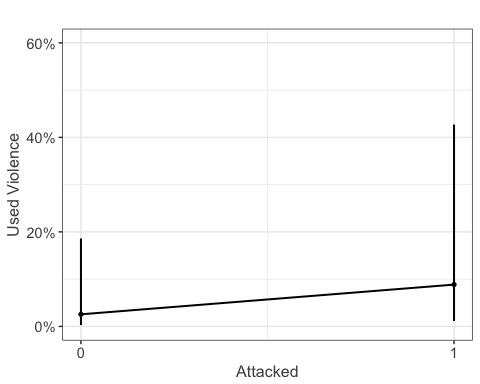
\includegraphics{dissertation_files/figure-latex/violplot-1.pdf}
\caption{\label{fig:violplot}Predicted Probability of the Use of Violence
(Model 1)}
\end{figure}

I also examine the effects of repression on three other forms of
political participation to shed light on alternative explanations. For
example, it may be the case that violent individuals are simply very
active in general, and thus have more opportunities than others to be
repressed. Comparative homebodies might see lower rates of repression
simply because they spend less time in public locations where repression
tends to occur, and any apparent association with lower levels of
political participation would likely be coincidental. In Model 3 I
examine voting. Repression measured at the individual level has a
negative relationship with voting. Individuals who reported an attack on
themselves or a family member were 20.4\% less likely than others to
have voted. The threat of election-related violence has a smaller, but
still statistically significant effect. At the national level better
human rights practices are associated with higher baseline rates of
voting, but the effect just misses the 90\% level of statistical
significance. These results suggest a potential explanation to the
puzzle of why governments use repression despite the negative
consequences I predict - it appears that repression is effective at
deterring individuals from voting, or at convincing them that politics
is unlikely to address their needs. For two more involved forms of
political action, however, attacks are associated with increased levels
of political participation. Experiencing an attack is associated with a
statistically significant, though substantively modest increase in the
probability than an individual has participated in community meetings,
as is the country-level human rights situation. The country-level
measure is not significantly related to protest activity, but being
attacked once again is, with individuals who have experienced an attack
being more than twice as likely to have participated in protest. It
should be noted, however, that the same endogeneity concerns that exist
for violence apply to these forms of participation as well, as these
results are consistent

\begin{table}
\begin{center}
\begin{tabular}{l c c c }
\hline
 & M3 Voting & M4 Meeting & M5 Protest \\
\hline
(Intercept)                             & $-5.60^{***}$ & $-2.29$       & $-2.81^{***}$ \\
                                        & $(0.43)$      & $(1.44)$      & $(0.51)$      \\
Human Rights                            & $0.13$        & $0.22^{*}$    & $-0.20$       \\
                                        & $(0.08)$      & $(0.09)$      & $(0.13)$      \\
Ethnolinguistic Fractionalization       & $-0.53$       & $-5.02$       & $2.12$        \\
                                        & $(1.65)$      & $(7.26)$      & $(1.89)$      \\
Ethnolinguistic Fractionalization$^{2}$ & $0.84$        & $5.59$        & $-0.85$       \\
                                        & $(1.61)$      & $(7.04)$      & $(1.84)$      \\
Polity                                  & $0.01$        & $0.22^{***}$  & $0.05^{*}$    \\
                                        & $(0.02)$      & $(0.02)$      & $(0.02)$      \\
Civil War                               & $0.07$        & $0.32^{***}$  & $-0.66^{***}$ \\
                                        & $(0.05)$      & $(0.05)$      & $(0.07)$      \\
Separatist War                          & $0.36$        & $0.74^{*}$    & $-0.37$       \\
                                        & $(0.33)$      & $(0.36)$      & $(0.42)$      \\
Attacked                                & $-0.15^{***}$ & $0.18^{***}$  & $0.82^{***}$  \\
                                        & $(0.03)$      & $(0.03)$      & $(0.04)$      \\
Intimidated                             & $-0.12^{***}$ & $0.03$        & $0.09^{**}$   \\
                                        & $(0.02)$      & $(0.02)$      & $(0.03)$      \\
Employed                                & $0.36^{***}$  & $0.12^{***}$  & $0.22^{***}$  \\
                                        & $(0.02)$      & $(0.02)$      & $(0.03)$      \\
Primary Education                       & $0.10^{***}$  & $0.13^{***}$  & $-0.38^{***}$ \\
                                        & $(0.02)$      & $(0.02)$      & $(0.03)$      \\
Urban                                   & $-0.06^{*}$   & $-0.06^{**}$  & $0.11^{**}$   \\
                                        & $(0.03)$      & $(0.02)$      & $(0.04)$      \\
Ruling Party Supporter                  & $0.24^{***}$  & $0.21^{***}$  & $-0.05$       \\
                                        & $(0.02)$      & $(0.02)$      & $(0.03)$      \\
Age                                     & $1.84^{***}$  & $0.67^{***}$  & $-0.16^{***}$ \\
                                        & $(0.03)$      & $(0.02)$      & $(0.03)$      \\
Female                                  & $-0.14^{***}$ & $-0.44^{***}$ & $-0.32^{***}$ \\
                                        & $(0.02)$      & $(0.02)$      & $(0.03)$      \\
\hline
AIC                                     & 62740.24      & 73422.70      & 37290.70      \\
BIC                                     & 62894.17      & 73576.62      & 37444.62      \\
Log Likelihood                          & -31353.12     & -36694.35     & -18628.35     \\
Num. obs.                               & 63222         & 63215         & 63195         \\
Num. groups: Ethnic:Country             & 650           & 650           & 650           \\
Num. groups: Country                    & 27            & 27            & 27            \\
Var: Ethnic:Country (Intercept)         & 0.07          & 0.16          & 0.12          \\
Var: Country (Intercept)                & 0.25          & 1.03          & 0.35          \\
\hline
\multicolumn{4}{l}{\scriptsize{$^{***}p<0.001$, $^{**}p<0.01$, $^*p<0.05$}}
\end{tabular}
\caption{Multilevel Models of Political Participation}
\label{tab:partic}
\end{center}
\end{table}

These results are robust to a number of adjustments. Changing the
cutpoints for the variables that I collapse into binary measures does
not substantially alter the results. Furthermore, leaving the violence
measure as a five-point scale and using an ordinal rather than standard
logit produces substantively similar results -- individuals who
experienced an attack are significantly more likely to report higher
levels of participation in violence (see Table \ref{tab:ordinal} in the
Chapter 3 Appendix). Adding the additional controls mentioned in the
research design does not alter the performance of my variables of
interest, nor does removing any control variables. As mentioned in the
research design section, I also explore the effects of several
additional control variables. The results are also robust to the
inclusion of random effects for the year in which the survey was
administered and the survey wave, and including these factors as fixed
effects rather than random results in only slight changes to the
magnitude of the relationships.

Collectively, these results allow me to reject the null hypothesis of no
relationship between repression and willingness to engage in violence
associated with \emph{H1}. Individuals who have been attacked are more
than three times more likely than others to engage in violence, and
roughly 20\% more likely to express a willingness to use violence. The
country-level human rights measure is not significantly related to
either outcome, however, suggesting that the effect of repression is
specific to the individuals who are targeted, and does not produce a
widespread spillover effect leading large swaths of society to change
their behavior. Several caveats must be noted, however. First, the
repression measure is imprecise, as individuals who experienced violence
personally are grouped with individuals with family members who
experienced violence, and the actor who perpetrated the attack is not
specified. Second, these results could be endogenous, with individuals
being attacked because they used or were known to be willing to use
violence. I address this possibility in Section \ref{causal}.

\hypertarget{ethnic-identification-results}{%
\section{Ethnic Identification
Results}\label{ethnic-identification-results}}

The ethnic identification results are reported in Table
\ref{tab:ethnic}. Model 5 includes a random intercept for each country,
while Model 6 adds an intercept for each ethnic group nested within each
country, and to that Model 7 adds a random intercept for year.\footnote{I
  use year instead of survey wave as the country-level variables are
  measured in yearly intervals.} In all three models, individuals who
have experienced an attack are more likely to identify with their ethnic
group than their nation, relative to individuals who have not
experienced an attack. This effect size is equivalent to a roughly 42\%
increase, a change in probability from 0.12 to 0.17 (see Figure
\ref{fig:ethplot1}), but is statistically significant at the 99.9\%
level. Political intimidation has a similar effect. The country-level
human rights measure is statistically significant in Models 5 and 6,
with a similar substantive effect. Among the most repressive cases in
the sample, individuals have a roughly 0.15 probability of identifying
with their ethnic group, with the probability decreasing to 0.10 among
the cases with the greatest respect for human rights (see Figure
\ref{fig:ethplot2}). The human rights variable is not significant in
Model 7, likely because as a relatively constant measure, it has little
ability to predict intercepts that vary by year.

\begin{table}
\begin{center}
\begin{tabular}{l c c c }
\hline
 & M5 & M6 & M7 \\
\hline
(Intercept)                             & $-4.43^{***}$ & $-4.34^{***}$ & $-3.44^{***}$ \\
                                        & $(0.65)$      & $(0.72)$      & $(0.43)$      \\
Human Rights                            & $-0.70^{***}$ & $-0.66^{***}$ & $0.12$        \\
                                        & $(0.12)$      & $(0.13)$      & $(0.11)$      \\
Ethnolinguistic Fractionalization       & $6.58^{*}$    & $6.38^{*}$    & $3.63^{*}$    \\
                                        & $(2.78)$      & $(3.18)$      & $(1.63)$      \\
Ethnolinguistic Fractionalization$^{2}$ & $-5.89^{*}$   & $-5.77$       & $-3.17^{*}$   \\
                                        & $(2.74)$      & $(3.11)$      & $(1.58)$      \\
Polity                                  & $0.15^{***}$  & $0.15^{***}$  & $0.03$        \\
                                        & $(0.02)$      & $(0.03)$      & $(0.02)$      \\
Civil War                               & $0.29^{***}$  & $0.33^{***}$  & $0.62^{***}$  \\
                                        & $(0.06)$      & $(0.06)$      & $(0.07)$      \\
Separatist War                          & $1.26^{**}$   & $1.61^{**}$   & $0.64$        \\
                                        & $(0.46)$      & $(0.53)$      & $(0.36)$      \\
Attacked                                & $0.25^{***}$  & $0.27^{***}$  & $0.23^{***}$  \\
                                        & $(0.04)$      & $(0.04)$      & $(0.04)$      \\
Intimidated                             & $0.23^{***}$  & $0.22^{***}$  & $0.20^{***}$  \\
                                        & $(0.03)$      & $(0.03)$      & $(0.03)$      \\
Employed                                & $-0.08^{**}$  & $-0.09^{**}$  & $-0.08^{**}$  \\
                                        & $(0.03)$      & $(0.03)$      & $(0.03)$      \\
Primary Education                       & $0.42^{***}$  & $0.41^{***}$  & $0.40^{***}$  \\
                                        & $(0.03)$      & $(0.03)$      & $(0.03)$      \\
Urban                                   & $-0.11^{***}$ & $-0.08^{*}$   & $-0.10^{**}$  \\
                                        & $(0.03)$      & $(0.03)$      & $(0.03)$      \\
Ruling Party Supporter                  & $-0.14^{***}$ & $-0.12^{***}$ & $-0.12^{***}$ \\
                                        & $(0.03)$      & $(0.03)$      & $(0.03)$      \\
Age                                     & $0.01$        & $-0.00$       & $-0.00$       \\
                                        & $(0.02)$      & $(0.02)$      & $(0.02)$      \\
Female                                  & $0.10^{***}$  & $0.10^{***}$  & $0.10^{***}$  \\
                                        & $(0.02)$      & $(0.03)$      & $(0.03)$      \\
\hline
AIC                                     & 45710.59      & 43941.95      & 43722.83      \\
BIC                                     & 45855.99      & 44095.82      & 43885.75      \\
Log Likelihood                          & -22839.29     & -21953.97     & -21843.41     \\
Num. obs.                               & 65384         & 63039         & 63039         \\
Num. groups: Country                    & 27            & 27            & 27            \\
Var: Country (Intercept)                & 0.57          & 0.51          & 0.15          \\
Num. groups: Ethnic:Country             &               & 650           & 650           \\
Var: Ethnic:Country (Intercept)         &               & 0.27          & 0.25          \\
Num. groups: Year                       &               &               & 5             \\
Var: Year (Intercept)                   &               &               & 0.09          \\
\hline
\multicolumn{4}{l}{\scriptsize{$^{***}p<0.001$, $^{**}p<0.01$, $^*p<0.05$}}
\end{tabular}
\caption{Multilevel Models of Ethnic Identification}
\label{tab:ethnic}
\end{center}
\end{table}

These results are robust to alternative specifications of the dependent
variable. Leaving the measure as a five-point scale in an ordinal logit
produces comparable results -- individuals who have been attacked have
statistically-significant of being closer to the ethnically-oriented end
of the scale (see Table \ref{tab:ordinal} in the Chapter 3 Appendix).
The control variables provide a number of interesting results. As I
expected, ethnolinguistic fractionalization has a substantively strong
and statistically significant curvilinear relationship with ethnic
identification in Models 5 and 7, and a linear one in Model 6 (indicated
by the squared term not being statistically significant). The
curvilinear pattern is consistent with my expectation that ethnic
identification will be unlikely at extreme levels of diversity.
Consistent with the findings of Eifert, Miguel, and Posner
(\protect\hyperlink{ref-Eifert2010}{2010}), Models 5 and 6 show that the
probability of ethnic identification increases as a country becomes more
democratic. Countries experiencing civil war have a somewhat higher
baseline level of ethnic identification, and the effect is considerable
for separatist wars. At the individual level, urban-dwellers, ruling
party supporters, and employed individuals are less likely to emphasize
an ethnic identity. Having at least a primary education increases the
probability that an individual with identify ethnically, and women are
slightly more likely than men to adopt such an identity.

\begin{figure}
\centering
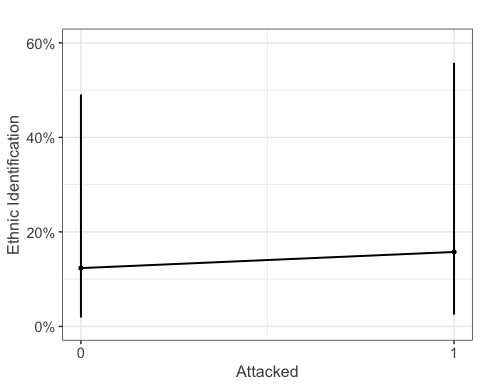
\includegraphics{dissertation_files/figure-latex/ethplot1-1.pdf}
\caption{\label{fig:ethplot1}Predicted Probability of Ethnic Identification
(Model 5)}
\end{figure}

\begin{figure}
\centering
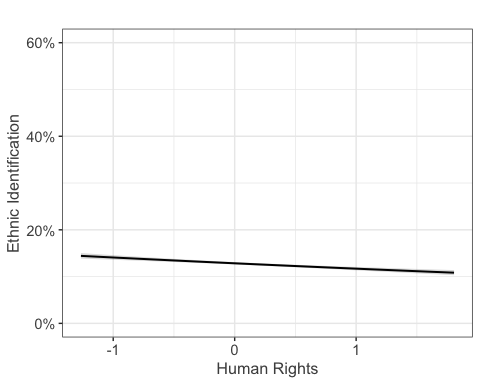
\includegraphics{dissertation_files/figure-latex/ethplot2-1.pdf}
\caption{\label{fig:ethplot2}Predicted Probability of Ethnic Identification
(Model 5)}
\end{figure}

While further analysis is need to establish the direction of the causal
relationship, these results do allow me to tentatively reject the null
hypothesis of no relationship between repression and ethnic
identification associated with \emph{H2}. Individuals who have been
attacked are more than 40\% more likely than others to identify with
their ethnic group. The country-level human rights measure tells a
similar story, with the probability of ethnic identification being lower
in countries with greater respect for human rights. As is the case with
the violence results, I cannot here rule out the possibility of
endogeneity. It is quite plausible that individuals who identify
strongly with an ethnic group are most likely to be targeted with
repression. Many governments repress ethnic minorities to prevent them
from undermining national unity. For example, the Turkish government has
denied the claim that the Kurds are a distinct ethnicity from Turks, and
have repressed them to prevent a secessionist movement. I address the
concern in the following section.

\hypertarget{causal}{%
\section{Causal Identification}\label{causal}}

As discussed above, the preceding results do not account for the
possibility of endogeneity. The ideal solution would be an instrumental
variable. However, a valid instrument would need to be a strong proxy
for repression, but only effect political participation and ethnic
identification through the effect of repression (this is known as the
exclusion restriction). Unfortunately, few if any measures included in
the Afrobarometer meet the requirements of a valid instrument. For
instance, previous work has often used distance from the capital to
instrument for an individual or location's probability of experiencing
violence (e.g. Voors et al. \protect\hyperlink{ref-Voors2012}{2012}).
While this measure may meet the exclusion restriction for some outcomes,
there is reason to believe that it does not for ethnic identification.
Robinson (\protect\hyperlink{ref-Robinson2014}{2014}) finds that
orientation toward national identities is driven in part by
modernization. Thus living in a remote location may affect ethnic
identification directly, rather than only through the variable it is
intended to instrument. At the country level democracy is strongly
correlated with repression (Davenport
\protect\hyperlink{ref-Davenport2007a}{2007}\protect\hyperlink{ref-Davenport2007a}{b}),
but also may have a direct effect on ethnic identification (Eifert,
Miguel, and Posner \protect\hyperlink{ref-Eifert2010}{2010}), and almost
certainly has one with political participation.

As an alternative to an instrument, I use coarsened exact matching
(Iacus, King, and Porro \protect\hyperlink{ref-Iacus2012}{2012}).
Matching seeks to create a subset of the data with a ``treatment'' (in
this case the individual-level attack variable) and ``control'' group
with similar values on a set of observable covariates. In this case I
seek to balance the sample on individual-level measures of education,
age, urban residence, support for the ruling party, and employment
status, and country-level measures of ethnolinguistic fractionalization,
Polity IV score, the Latent Human Protection Scores, and indicators for
the presence of civil and separatist wars. Coarsened exact matching
achieves balance by collapsing each continuous and categorical variable
into a smaller number of strata, and identifying pairs of treated and
control units that fall into the same strata on each variable. While
there was a statistically significant difference of means between the
treated and control groups on each of the covariates prior to matching,
there are no significant differences on any variable after matching, and
the mean difference between the groups reduces to zero for each variable
except age and the categorical education measure, which each differ by
less than 0.1. The trade-off for pursuing such exact matches is a loss
of observations, as cases with no close are match are discarded. The
problem is not especially dire in this case, however, as the number of
cases reduces from 38,681 (the number of cases with no missing values on
any covariate) to 28,251. The limitation of matching is its inability to
address unobservable sources of bias. Thus, if certain individuals are
disproportionately likely to be attacked for reasons that are not
entirely captured by the included covariates, this bias is likely to
remain in the post-matching sample.

\begin{table}
\begin{center}
\begin{tabular}{l c c c }
\hline
 & M8 Violence (Willing) & M9 Violence (Used) & M10 Ethnic ID \\
\hline
Human Rights                            & $0.05$        & $0.08$        & $-0.19$       \\
                                        & $(0.17)$      & $(0.25)$      & $(0.13)$      \\
Ethnolinguistic Fractionalization       & $1.33$        & $-0.44$       & $4.99^{**}$   \\
                                        & $(2.04)$      & $(3.04)$      & $(1.63)$      \\
Ethnolinguistic Fractionalization$^{2}$ & $-1.01$       & $1.60$        & $-4.78^{**}$  \\
                                        & $(2.06)$      & $(3.04)$      & $(1.62)$      \\
Polity                                  & $-0.04$       & $-0.01$       & $-0.03$       \\
                                        & $(0.03)$      & $(0.04)$      & $(0.02)$      \\
Civil War                               & $0.21$        & $-0.44^{*}$   & $0.13$        \\
                                        & $(0.20)$      & $(0.20)$      & $(0.19)$      \\
Separatist War                          & $-0.17$       & $-0.82$       & $0.30$        \\
                                        & $(0.53)$      & $(0.86)$      & $(0.43)$      \\
Attacked                                & $0.47^{***}$  & $1.09^{***}$  & $0.26^{***}$  \\
                                        & $(0.07)$      & $(0.08)$      & $(0.06)$      \\
Intimidated                             & $0.14^{*}$    & $0.11$        & $0.29^{***}$  \\
                                        & $(0.05)$      & $(0.08)$      & $(0.04)$      \\
Employed                                & $-0.05$       & $-0.06$       & $-0.00$       \\
                                        & $(0.06)$      & $(0.08)$      & $(0.05)$      \\
Primary Education                       & $0.01$        & $0.16^{*}$    & $0.39^{***}$  \\
                                        & $(0.05)$      & $(0.08)$      & $(0.05)$      \\
Urban                                   & $-0.17^{*}$   & $-0.19^{*}$   & $-0.06$       \\
                                        & $(0.07)$      & $(0.09)$      & $(0.06)$      \\
Ruling Party Supporter                  & $-0.08$       & $-0.14^{*}$   & $-0.16^{***}$ \\
                                        & $(0.05)$      & $(0.07)$      & $(0.04)$      \\
Age                                     & $-0.22^{***}$ & $0.01$        & $-0.07$       \\
                                        & $(0.06)$      & $(0.08)$      & $(0.05)$      \\
Female                                  & $-0.22^{***}$ & $-0.31^{***}$ & $0.04$        \\
                                        & $(0.05)$      & $(0.07)$      & $(0.04)$      \\
\hline
AIC                                     & 13661.19      & 7297.64       & 18584.48      \\
BIC                                     & 13801.42      & 7437.88       & 18724.71      \\
Log Likelihood                          & -6813.60      & -3631.82      & -9275.24      \\
Num. obs.                               & 28251         & 28251         & 28251         \\
Num. groups: Ethnic:Country             & 497           & 497           & 497           \\
Num. groups: Country                    & 26            & 26            & 26            \\
Var: Ethnic:Country (Intercept)         & 0.19          & 0.39          & 0.30          \\
Var: Country (Intercept)                & 0.16          & 0.35          & 0.09          \\
\hline
\multicolumn{4}{l}{\scriptsize{$^{***}p<0.001$, $^{**}p<0.01$, $^*p<0.05$}}
\end{tabular}
\caption{Models with Matched Data}
\label{tab:matching}
\end{center}
\end{table}

The results using the matched data are reported in Table
\ref{tab:matching}, and the estimates for the attack variable are very
similar to those seen in the raw data. Individuals who have experienced
an attack are substantially more likely to express willingness to engage
in violence, with the effect being statistically significant at the
99.9\% level (Model 8). The substantive effect is modest, however,
increasing the probability from 0.08 to 0.11 (see Figure
\ref{fig:matchviolplotwilling}). These individuals also report higher
probabilities of having engaged in violence, and the effect is
significant at the 99.9\% level (Model 9). Individuals who have been
attacked are three times more likely than others to have used violence
themselves (0.09 vs.~0.03, see Figure \ref{fig:matchviolplot}).
Additionally, being attacked is associated with a modest increase (0.14
vs.~0.11, see Figure \ref{fig:matchethplot}) in the probability of
ethnic identification, which is again significant at the 99.9\% level.
Many of the covariates are no longer significant after matching, as
attack and non-attack subsets have identical means on these variables.

\begin{figure}
\centering
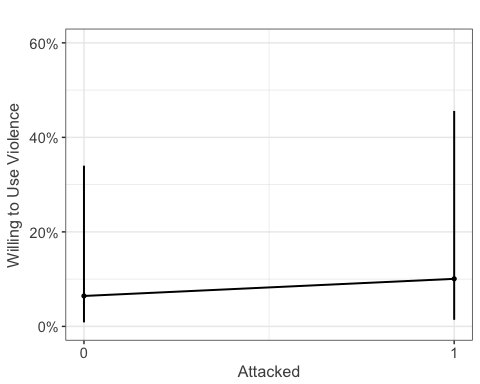
\includegraphics{dissertation_files/figure-latex/matchviolplotwilling-1.pdf}
\caption{\label{fig:matchviolplotwilling}Predicted Probability of the Use of
Violence (Model 8)}
\end{figure}

\begin{figure}
\centering
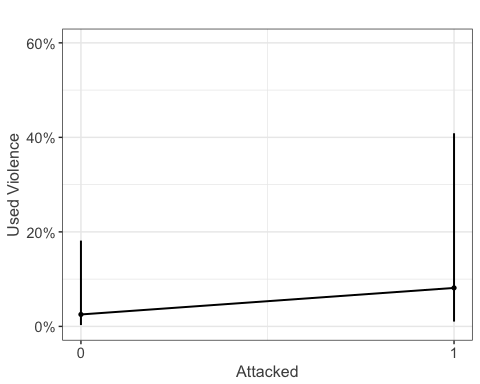
\includegraphics{dissertation_files/figure-latex/matchviolplot-1.pdf}
\caption{\label{fig:matchviolplot}Predicted Probability of the Use of
Violence (Model 8)}
\end{figure}

As noted above, matching cannot guard against all potential threats to
causal inference. If some individuals are disproportionately likely both
to be attacked and to engage in violence or identify ethnically for
reasons that are not captured by the covariates, this bias will remain.
One might imagine, however, that governments (and other actors) often
make decisions of who to repress based on the sort of observable
characteristics such as age and sex that are included in the matching.
The matching analysis ensures that these observable measures do not bias
the results. Thus while there is still some possibility of endogeneity,
these results should increase our confidence that individuals who are
attacked are not systematically different from others.

\begin{figure}
\centering
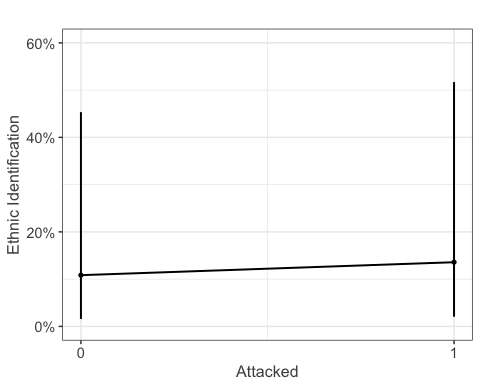
\includegraphics{dissertation_files/figure-latex/matchethplot-1.pdf}
\caption{\label{fig:matchethplot}Predicted Probability of Ethnic
Identification (Model 9)}
\end{figure}

\hypertarget{survey-conclusion}{%
\section{Conclusion}\label{survey-conclusion}}

The results in this chapter provide strong support for the
microfoundations of my theory. I expected that repression would make
individuals more willing to engage in violence. Consistent with this
hypothesis, I find that while such sentiments are generally rare,
individuals who have experienced a violent attacked are roughly 30\%
more likely than others to report a willingness to use violence, and are
nearly three times more likely to report having used violence. I also
predicted that repression should induce greater levels of ethnic
identification among its targets. Indeed, I find that individuals who
have experienced an attack are 42\% more likely than others to identify
more with their ethnic group than with their nation. The results hold
after conducting coarsened exact matching, meaning that the results are
not driven by any observable differences between the individuals who
have been attacked and those who have not.

This analysis has several important practical and theoretical
implications. First, it suggests that repression is often
counterproductive. Presumably, governments use repression to mitigate
and deter threats to their rule. Yet, my findings suggest that
repression could \emph{increase} the number of individuals using
violence, and entrench identities that could form the basis of an
opposition to the government. As discussed in Chapter @ref(\#theory),
this makes the government's use of repression puzzling. My other
findings on political participation hint at an answer, however.
Repression does seem to reduce the probability than individual will
vote, suggesting that governments may be accepting increased numbers of
violent individuals in exchange for the opportunity to shape the
electorate. Second, the results suggest that repression can trigger a
vicious cycle, in which the government responds to an initial threat in
a way that further entrenches the opposition, leading to ever-greater
levels of violence.

In the remaining chapters, I build on the foundations established here
to explain variations at the level of the rebel movement. I find
evidence that the dynamics discussed here shape the formation of new
rebel groups, the fragmentation of existing ones, and the formation of
alliances between previously independent groups.

\hypertarget{entry}{%
\chapter{The Formation of New Rebel Groups}\label{entry}}

This chapter builds on the individual-level findings from Chapter
\ref{survey-chapter} to explain one aggregate manifestation of
repression --- the formation of entirely new rebel groups. Specifically,
I am interested in cases where entirely new rebel groups join ongoing
civil wars. By new I simply mean a group that has not previously
participated in violence. Pre-existing non-violent organizations such as
religious organizations or political parties could constitute a new
rebel group so long as they have not used violence previously, as would
entirely new organizations that form during a conflict. I distinguish
this sort of group formation from the splintering of existing
organizations, as I expect the causal processes to be somewhat
different. While splintering is driven by individuals who have already
resorted to violence deciding to reorganize, group formation has the
additional requirement of mobilizing previously non-violent individuals.
To the best of my knowledge, no existing study directly addresses this
question.

I expect that repression should increase the probability that a new
rebel group will enter an ongoing conflict. As previously peaceful
individuals experience violence, the relative cost for them to join a
rebellion decreases. These individuals will not necessarily be inclined
to join an existing rebel group, however. If an individual has been
repressed, existing groups have in some sense failed to protect them.
Furthermore, repression should tend to induce greater levels of ethnic
identification. Repression is often targeting on the basis of ethnicity,
increasing the salience of such identities. Ethnic identification may
also have instrumental value in attracting support from outside
co-ethnic states, and repression may give these outside states both
motive and political cover for supporting new rebel groups. Thus, there
should be a relationship between repression and the emergence of new
rebel groups.

\emph{Hypothesis 3: The probability that a new rebel group will form
should increase with the level of repression in the country}

If ethnic polarization is the mechanism behind rebel group formation,
the ethnic diversity of a country should provide an important scope
condition. It would be unlikely for repression to induce ethnic
identification in a very homogeneous society, for instance. In such
cases a different social cleavage might be activated, or repression
might not sow division among dissidents at all. I thus expect a positive
interaction between repression and ethnic diversity, with repression
increasing the probability of new rebel groups at higher levels of
diversity, while being less effective at low levels of diversity.

\emph{Hypothesis 4: There should be a positive interaction between
repression and ethnic diversity}

My theory suggests that individuals form new rebel groups largely
because repression begins to polarize society on the dimension of ethnic
identity. This argument has a testable implication regarding the new
rebel groups that emerge --- they should be likelier than pre-existing
groups to draw their support from a single ethnic group.

\emph{Hypothesis 5: Rebel groups that join ongoing conflicts should be
more likely than others to draw their support from a single ethnic
group}

\hypertarget{research-design-1}{%
\section{Research Design}\label{research-design-1}}

To test the preceding hypotheses I use a dataset of conflict-years
derived from the Uppsala Conflict Data Program and Peace Research
Institute Oslo's Dyadic Dataset, version 4-2016 (Harbom, Melander, and
Wallensteen \protect\hyperlink{ref-Harbom2008}{2008}; Melander,
Pettersson, and Themnér \protect\hyperlink{ref-Melander2016}{2016}).
This dataset includes one observation for every government-rebel group
dyad for each year in which it produced at least 25 fatalities. I
exclude all interstate conflicts from the data, and include all civil
wars, anti-colonial wars, and internationalized civil wars. The
remaining rebel dyads are grouped into conflicts, with all rebels
seeking to overthrown the central government considered to be part of
the same conflict, and separatist movements grouped together if they are
pursuing independence for the same territory. Thus conflicts can contain
multiple rebel groups, and countries can contain multiple conflicts. I
then aggregate this data to the conflict-year, as my outcome of interest
is whether a new rebel group joined the fighting in a given year. This
results in a dataset of 2,048 observations, covering the period
1946--2015.

The advantage of using conflict-years rather than aggregating to
country-years is that I am able to examine the effects of several
covariates measured at the conflict level, including conflict intensity
and the type of issue at stake. Disaggregating to the conflict level,
rather than the country also avoids conflating situations in which
multiple rebel groups compete for similar objectives from those in which
multiple rebel groups form for completely different purposes. Using
yearly observations rather than a single count for each conflict is
useful because the number of rebel groups tends to vary over time, and
thus a yearly count allows me to identify factors that can account for
the timing of new group formation, rather than only cross-sectional
correlates. The use of conflict-years does create a methodological
challenge, however, as many of my covariates are measured at the country
level. To combat this I cluster the standard errors by country.
Additionally, aggregating the data to the country-year does not
substantially change the results.

\hypertarget{dependent-variables-1}{%
\subsection{Dependent Variables}\label{dependent-variables-1}}

\hypertarget{entry-of-new-rebel-groups}{%
\subsubsection*{Entry of New Rebel
Groups}\label{entry-of-new-rebel-groups}}
\addcontentsline{toc}{subsubsection}{Entry of New Rebel Groups}

My primary dependent variable in this study is the entry of new rebel
groups to an ongoing conflict. To qualify, a rebel group must meet two
criteria. First, it cannot have previously participated in political
violence. To determine this I use rebel origins data I collected
(described in the Chapter 2 Appendix), and exclude groups that
originated as portions of different rebel groups --- splinter
organizations and alliances. This leaves rebel groups that emerged out
of non-violent organizations such as political organizations, as well as
militarized, but not political organizations such as local defense
militias. Second, the group must join an ongoing conflict. I define a
conflict as ongoing if it has produced at least 25 fatalities in at
least one of the past three years. If three consecutive years of peace
occur, I consider the next round of fighting to be a new conflict
episode, and any new rebel groups that appear in the first year of an
episode are considered to have initiated that conflict rather than
joined it.

Of the 503 rebel groups that appear in my data, 83 fit the definition.
As some of these entered the same conflict in the same year, 73 of
2045\footnote{Some observations are left-censored, meaning I am unable
  to determine whether there was conflict during the previous three
  years as it would predate the beginning of the dataset.} (5.6\%) of
conflict-years are coded as having a new rebel group.

\hypertarget{rebel-group-ethnicity}{%
\subsubsection*{Rebel Group Ethnicity}\label{rebel-group-ethnicity}}
\addcontentsline{toc}{subsubsection}{Rebel Group Ethnicity}

\emph{H5} predicts that because the formation of new rebel groups is
driven by a broader reorganization of society along ethnic lines, these
newly-formed rebel groups should be likelier than others to draw their
support from a single ethnic group. To test this I use the ACD2EPR 2014
dataset (Wucherpfennig et al.
\protect\hyperlink{ref-Wucherpfennig2011}{2011}; Vogt et al.
\protect\hyperlink{ref-Vogt2015}{2015}), which links rebel groups from
the Uppsala Armed Conflict Data v.4-2014 (Melander, Pettersson, and
Themnér \protect\hyperlink{ref-Melander2016}{2016}) to ethnic groups
from the Ethnic Power Relations (EPR-Core 2014) (Cederman, Wimmer, and
Min \protect\hyperlink{ref-Cederman2010}{2010}; Vogt et al.
\protect\hyperlink{ref-Vogt2015}{2015}). This dataset identifies three
forms of linkages between ethnic groups and rebel groups. First, a rebel
group can claim to operate exclusively on behalf of a particular ethnic
group. The dataset does allow for the possibility that a group could
make such claims for multiple ethnic groups, as was the case for several
of the South Sudanese separatist groups. Second, the data records all of
the ethnic groups from which a rebel group recruits a significant number
of soldiers. Finally, the data codes whether at least 50\% of the
members of an ethnic group support a rebel group. I collapse these
measures into a single count of the number of ethnic groups to which a
rebel group is tied. I then categorize rebel groups as ``mono-ethnic,''
``multi-ethnic,'' or ``non-ethnic,'' if they have no such ties. The
distribution of cases across these categories is reported in Table
\ref{tab:acd2epr}.

\begin{longtable}[]{@{}lll@{}}
\caption{\label{tab:acd2epr} Rebel Groups by Ethnic
Affiliation}\tabularnewline
\toprule
Non-Ethnic & Mono-Ethnic & Multi-Ethnic\tabularnewline
\midrule
\endfirsthead
\toprule
Non-Ethnic & Mono-Ethnic & Multi-Ethnic\tabularnewline
\midrule
\endhead
97 & 309 & 47\tabularnewline
\bottomrule
\end{longtable}

\hypertarget{independent-variables-1}{%
\subsection{Independent Variables}\label{independent-variables-1}}

\hypertarget{human-rights}{%
\subsubsection*{Human Rights}\label{human-rights}}
\addcontentsline{toc}{subsubsection}{Human Rights}

To measure repression I use the same country-level measure employed in
Chapter \ref{survey-chapter}, the Latent Human Protection scores,
version 2 (Fariss \protect\hyperlink{ref-Fariss2014}{2014}; Schnakenberg
and Fariss \protect\hyperlink{ref-Schnakenberg2014}{2014}). The
motivation for this data project is the fact that human rights measures
are typically based on media reports, creating the possibility that both
the depth of coverage and standards against which human rights practices
are evaluated might vary across space and time. To solve this, the
dataset uses thirteen data sources including U.S. State Department and
Human Rights Watch reports and most major scholarly datasets in a
Bayesian measurement model. This produces an estimate for each
country-year based on a mix of the data for that particular year and the
average score for that country and year. While this creates a human
rights measure that is comparable across contexts, one disadvantage is
that the units are not inherently meaningful, only providing a basis for
comparison across observations.

The measure ranges from roughly -3.1 (most repressive) to 4.7 (most
respectful of human rights). The average score across the full sample of
post-World War II country-years is 0.29, while in my sample of countries
experiencing civil war the mean is -1.24, with a range from -3.11 to
1.51. Thus, the sample includes the full range of repressive states,
while unsurprisingly lacking any states with especially strong human
rights practices. For reference, recent country-years with scores around
1.5 including Hungary in 2011, and France in 2007. In other words, these
are typically cases in which citizens are generally safe from physical
harm, but some minorities such as Muslims in France experience political
and economic discrimination. Russia in recent years falls in the middle
of the spectrum, with scores around 1.0. Examples of cases towards the
more repressive end of the spectrum include Saddam Hussein's Iraq, which
had a score averaging around -2.5, and Sudan, which had scores around
-3.0 during the genocide in Darfur.

The raw Latent Human Protection Scores tend to be relatively static over
time. Yet, my theory suggests that it is changes in human rights
practices, in the direction of being more repressive, that should change
dissident behavior. To ensure that I am capturing these phenomena, I use
the year-over-year change in human protection score. While the average
conflict-year sees very little change from the preceding year (the mean
change is -0.01), 110 cases experience a negative change of at least
0.25, and in one case the score decreased by 2.52 in a single year. I
lag the measure by one year, meaning that I am ultimately using the
change in human rights practices at time \emph{t} to predict the
formation of new rebel groups at time \emph{t+1}.

\hypertarget{ethnic-diversity}{%
\subsubsection*{Ethnic Diversity}\label{ethnic-diversity}}
\addcontentsline{toc}{subsubsection}{Ethnic Diversity}

\emph{H4} suggests that ethnic diversity should place a scope condition
on my theory, with the formation of new groups being less likely at very
high and low levels of ethnic diversity. I first test for the effect of
ethnic diversity individually by including the raw and squared
ethnolinguistic fractionalization as predictors. This tests for a
curvilinear relationship, allowing for the effect of the variable to
differ at moderate and extreme values. The data come from Fearon and
Laitin (\protect\hyperlink{ref-fearonlaitin03}{2003}), and can be
interpreted as the probability that two individuals drawn at random will
be able to communicate. In addition to testing whether ethnic diversity
affects the probability of new group formation on its own, I also test
whether it alters the performance of the human rights measure, by
interacting the latter with both the raw and squared ethnolinguistic
fractionalization measures.

\hypertarget{new-rebel-group-entry}{%
\subsubsection*{New Rebel Group Entry}\label{new-rebel-group-entry}}
\addcontentsline{toc}{subsubsection}{New Rebel Group Entry}

\emph{H5} predicts that the rebel groups that form during ongoing
conflicts should be more likely than others to be tied to a single
ethnic group. Thus the new rebel group entry variable becomes an
independent variable in this analysis, predicting the ethnic composition
of rebel groups.

\hypertarget{control-variables-1}{%
\subsection{Control Variables}\label{control-variables-1}}

I control for several factors that might confound my results. To account
for the possibility that human rights scores are simply a function of
conflict intensity, rather than discriminatory intent, I include the
maximum conflict intensity value from the UCDP Dyadic data. The measure
is binary, with a value of 1 indicating that the dyad produced between
25 and 999 fatalities in a given year, and a value of 2 indicating that
the dyad produced 1,000 or more fatalities. This measure is moderately
correlated with the human rights score (Pearson's r = -0.30). The exact
measure of fatalities available for the post-1989 period is even less
correlated (Pearson's r = -0.25). Thus, human rights practices are for
the most part measuring something distinct from conflict intensity.

Conflicts that already have multiple rebel groups may have some
unobserved quality that makes them more likely to have fragmented rebel
movements. For example, there might be a history of personal animosity
between rebel elites (see Christia
\protect\hyperlink{ref-Christia2012}{2012}). To capture such effects, I
include a binary indicator of whether a conflict had multiple rebel
groups in the previous year.

Two standard controls from past conflict studies are also likely to be
relevant. One potential mechanism that might produce increased numbers
of rebel groups in a conflict is the movement of groups from a
neighboring civil war into a new conflict. To control for this
possibility I construct an indicator for the presence of a civil war in
a state that is contiguous by land using the UCDP Dyadic data and the
Correlates of War Direct Contiguity data, version 3.2 (Stinnett et al.
\protect\hyperlink{ref-Stinnett2002a}{2002}). As secessionist movements
are often (though not always) tied to a specific ethnic group, my
hypothesized theoretical mechanism should be less likely to apply in
such conflicts. Thus, I include a binary indicator of whether a conflict
is secessionist as opposed to being fought over control of the central
government.

I also control for several country-level factors. Conceivably, the
number of rebel groups in a country might simply be a function of the
country's size. I thus include a measure of the countries area in logged
square kilometers from the World Bank (The World Bank
\protect\hyperlink{ref-WorldBank2015}{2015}), and logged population and
logged GDP per capita from Gleditsch
(\protect\hyperlink{ref-Gleditsch2002b}{2002}). The characteristics of a
country's terrain might also matter, with mountainous areas both
creating more opportunities for rebellion, and more challenges in
coordinating rebel activities across space. To control for this affect I
include Fearon and Laitin's (2003) measure of the percentage of a
country's terrain that is mountainous. As democratic competition might
provide another incentive for ethnic identification (Eifert, Miguel, and
Posner \protect\hyperlink{ref-Eifert2010}{2010}), I include the
country's Polity IV regime score (Marshall, Gurr, and Jaggers
\protect\hyperlink{ref-Marshall2016}{2016}). The international context
could conceivably play an important role in rebel group formation, for
instance by shaping the availability of external support. I thus include
a binary indicator of whether a country-year occurred during or after
the Cold War.

Finally, the presence of natural resources may influence the functioning
of my theoretical mechanism. My theory assumes that rebel elites desire
the support of dissident constituents. If rebel groups are able to
procure sufficient funds and war materiel through the sale of natural
resources, however, they might care little about civilians (see
Weinstein \protect\hyperlink{ref-Weinstein2007}{2007}). I thus include a
count of the number of locations in a country containing `lootable'
natural resources, meaning those which can be extracted with relatively
unsophisticated operations. The resources included in the measure are
oil (Lujala, Rød, and Thieme \protect\hyperlink{ref-Lujala2007}{2007}),
diamonds (Gilmore et al. \protect\hyperlink{ref-Gilmore2007}{2005};
Lujala, Gleditsch, and Gilmore
\protect\hyperlink{ref-Lujala2005}{2005}), gold (Balestri
\protect\hyperlink{ref-Balestri2012}{2012}), gems (Lujala
\protect\hyperlink{ref-Lujala2008}{2008}), and drugs (Buhaug and Lujala
\protect\hyperlink{ref-Buhaug2005}{2005}).

\hypertarget{statistical-model}{%
\subsection{Statistical Model}\label{statistical-model}}

As the dependent variable in this study is a binary measure of whether a
new rebel group entered a conflict in a given year, I use a logistic
regression model. While I examine the influence of each of the control
variables listed above, I also fit models with only the controls that
are statistically-significant or that substantially alter the
performance of my independent variables. This practice is consistent
with the advice of Achen (\protect\hyperlink{ref-Achen2002a}{2002}) and
Ray (\protect\hyperlink{ref-Ray2003}{2003}), who caution that including
too many covariates can obscure meaningful patterns and inhibit thorough
vetting of model assumptions. For robustness, I examine several variants
of the model. These include a model with fixed effects for country and
year, and a rare-events correction to account for the fact that group
formation occurs in only a small portion of my cases. I also cluster the
standard errors by country, as many of my variables are measured at the
country-level, creating the possibility that errors could be correlated
across different conflicts in the same country. I also estimate models
(not reported) with the country-year as the unit of analysis. None of
these changes substantially alters the results for my variables of
interest.

\hypertarget{results}{%
\section{Results}\label{results}}

\hypertarget{group-formation-results}{%
\subsection{Group Formation Results}\label{group-formation-results}}

The logistic regression results are reported in Table \ref{tab:entry}.
Model 1 includes only the change in human rights measure, Model 2 adds a
battery of controls, Model 3 includes an interaction effect between
human rights and ethnolinguistic fractionalization, and Model 4 replaces
the (mostly) static country-level variables with fixed effects for
conflict and year.

In the three models without interaction terms the Change in Human Rights
variable performs as I expect. It has a consistent, negative
relationship with the probability of new rebel group formation. As human
rights improve, the probability that new rebel groups will form
decreases, while increases in repression increase the probability of new
groups forming. The relationship is statistically significant at the
99\% level in all three models. The substantive effect is large, with a
one-unit (which equates to roughly 1.5 standard deviations) decrease in
human rights practices being associated with a roughly 400\% increase in
the odds of new rebel group formation. While the predicted probability
of a new rebel group emerging is quite low when the change in human
rights practices is zero (around 0.03, see Figure \ref{fig:effectplot}),
at the largest decreases (a change of -2.5 in one year) the probability
of a new rebel group emerging is 0.72. The effect size is similar across
models. With these results I am able to reject the null hypothesis of no
relationship between repression and the formation of new rebel groups,
consistent with my expectation in \emph{Hypothesis 4}.

\begin{table}
\begin{center}
\begin{tabular}{l c c c c }
\hline
 & Model 1 & Model 2 & Model 3 & Model 4 \\
\hline
(Intercept)                       & $-3.27^{***}$ & $5.79^{*}$   & $5.59$      & $15.71$      \\
                                  & $(0.13)$      & $(2.91)$     & $(2.96)$    & $(14503.27)$ \\
Change in Human Rights            & $-1.37^{***}$ & $-1.39^{**}$ & $-3.31^{*}$ & $-1.79^{**}$ \\
                                  & $(0.33)$      & $(0.43)$     & $(1.29)$    & $(0.59)$     \\
Ethnolinguistic Fractionalization &               & $0.23$       & $0.61$      &              \\
                                  &               & $(0.86)$     & $(0.91)$    &              \\
Human Rights X Fractionalization  &               &              & $3.32$      &              \\
                                  &               &              & $(2.09)$    &              \\
Intensity Level                   &               & $-0.23$      & $-0.25$     & $-0.23$      \\
                                  &               & $(0.39)$     & $(0.40)$    & $(0.44)$     \\
Prev. Multi-rebel                 &               & $0.23$       & $0.25$      & $-0.95^{**}$ \\
                                  &               & $(0.38)$     & $(0.38)$    & $(0.36)$     \\
Contiguous Civil War              &               & $-0.07$      & $-0.08$     & $0.29^{*}$   \\
                                  &               & $(0.10)$     & $(0.11)$    & $(0.14)$     \\
Secessionist                      &               & $-1.21^{**}$ & $-1.13^{*}$ &              \\
                                  &               & $(0.44)$     & $(0.45)$    &              \\
Logged Area                       &               & $-0.25$      & $-0.23$     &              \\
                                  &               & $(0.19)$     & $(0.19)$    &              \\
Mountainous Terrain               &               & $-0.00$      & $0.00$      &              \\
                                  &               & $(0.01)$     & $(0.01)$    &              \\
Logged GDP per capita             &               & $-0.38$      & $-0.39$     &              \\
                                  &               & $(0.24)$     & $(0.24)$    &              \\
Logged Population                 &               & $-0.22$      & $-0.24$     &              \\
                                  &               & $(0.24)$     & $(0.24)$    &              \\
Polity                            &               & $0.01$       & $0.01$      &              \\
                                  &               & $(0.03)$     & $(0.03)$    &              \\
Post Cold War                     &               & $-0.21$      & $-0.18$     &              \\
                                  &               & $(0.38)$     & $(0.38)$    &              \\
Lootable Resource Sites           &               & $-0.01$      & $-0.01$     &              \\
                                  &               & $(0.01)$     & $(0.01)$    &              \\
\hline
AIC                               & 521.11        & 319.37       & 318.68      & 585.79       \\
BIC                               & 531.86        & 389.01       & 393.30      & 1263.99      \\
Log Likelihood                    & -258.55       & -145.69      & -144.34     & -164.90      \\
Deviance                          & 517.11        & 291.37       & 288.68      & 329.79       \\
Num. obs.                         & 1597          & 1069         & 1069        & 1478         \\
\hline
\multicolumn{5}{l}{\scriptsize{$^{***}p<0.001$, $^{**}p<0.01$, $^*p<0.05$}}
\end{tabular}
\caption{Logit Models of Rebel Group Formation}
\label{tab:entry}
\end{center}
\end{table}

Model 3 provides a test of the interaction proposed in \emph{H5}.
Whereas I expect an interaction effect between the human rights measure
and ethnolinguistic fractionalization, the interaction is not
statistically significant. Ethnic diversity does not seem to matter on
its own, either, as there is no evidence of a curvilinear effect, nor of
a linear effect (not reported). I am thus unable to reject the null
hypothesis of no relationship between ethnic diversity and the
probability of new rebel groups forming. I also test for a curvilinear
relationship between ethnolinguistic fractionalization and rebel group
formation, and an interaction between human rights and the curvilinear
measure. Neither is statistically significant. It is unclear whether
this means my hypothesized mechanism of increased ethnic salience
operates even at extreme levels of diversity, or if other mechanisms
might operate in those cases. The analysis later in this chapter sheds
light on that question.

\begin{figure}
\centering
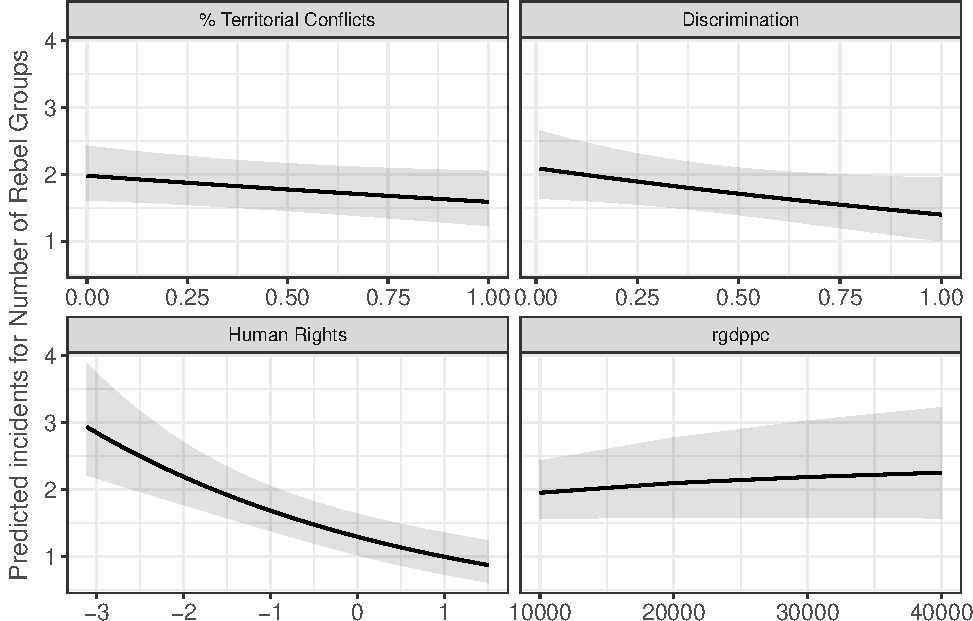
\includegraphics{dissertation_files/figure-latex/effectplot-1.pdf}
\caption{\label{fig:effectplot}Predicted Probability of New Rebel Group
Formation (Based on Model 2)}
\end{figure}

Only a few control variables are significant, likely reflecting the fact
that rebel group formation is a rare and time-varying outcome, while
many of the predictors are largely static. New rebel groups are less
likely in secessionist conflicts. As these conflicts are often fought by
an ethnically homogeneous movement, this result is consistent with my
overarching belief that the formation of new groups is about fighting on
behalf of previously underrepresented ethnic groups. The `Previously
Multi-Rebel' measure is negatively related the probability of further
groups joining, though only in the fixed effects model. This result
perhaps suggests that rather than portending further fragmentation of
the rebel movement, the presence of multiple rebel groups might signal
that a conflict has become saturated with factions, and further
additions are unlikely. Contiguous civil wars have a significant
positive relationship, suggesting that some new rebel groups might be
transnational in character. Again, however, the result is only
significant in the fixed effects model.

These results are robust to a number of manipulations. The raw Latent
Human Protection Score also consistently predicts the formation of new
groups, though the substantive effect is slightly smaller than that of
the differenced measure I employ. As mentioned, the results are similar
when the data are aggregated into conflict years rather than treating
separatist movements as distinct conflicts. I also include attributes of
the largest rebel group active in the previous year, such as its size,
degree of centralization, and whether it received foreign support. None
change the performance of my human rights measure.

The core results also hold when disaggregating observations by severity
(see the Chapter 4 Appendix). Among conflict-years with at least 25 but
fewer than 1,000 battle-related fatalities, the results are
substantively identical to those drawing on the full sample (Table
\ref{tab:entry-conflict}). The lagged, differenced human rights measure
has a statistically-significant, negative relationship with the
formation of new groups across a variety of model specifications. Within
the category of wars (years with 1,000 or more fatalities), the results
are similar, with the exceptions that the relationship is not
statistically-significant in a model with fixed effects for conflict and
year (Table \ref{tab:entry-wars}), and the interaction between
repression and ethnolinguistic fractionalization is statistically
significant.

The results do substantially differ, however, between different types of
rebellions. Conflicts over control of the central government exhibit
similar patterns to the full sample of conflicts, with the change in
human rights measure having a consistent negative relationship with the
probability of new group formation (Table \ref{tab:entry-govt}). Among
secessionist conflicts, however, the relationship is not
statistically-significant in any specification (Table
\ref{tab:entry-sec}). In light of my theory, however, this discrepancy
is not entirely surprising. My framework suggests that repression should
induce individuals to identify more strongly with their ethnic group.
Whereas campaigns to overthrow the central government are often diverse
and therefore might produce multiple ethnically-focused rebel groups,
secessionist movements are often organized around ethnic identity, and
thus we should not expect to see many new rebel groups form through this
mechanism.

I do not perform any sort of causal identification in this analysis. I
have examined several measures of oil production as potential
instruments for repression, but none came close to the conventional
standard for a strong instrument.\footnote{An instrument is considered
  strong if the first-stage F-statistic is at least 10 (Angrist and
  Pischke \protect\hyperlink{ref-Angrist2009}{2009}). The scores for the
  oil measures were generally around 4.5.} Matching is not an ideal
choice here, as it requires a binary treatment, and my human rights
measure is continuous. I cannot rule out the possibility that my results
actually reflect the government's ability to anticipate new rebellions.
Given that a rebel group must produce 25 fatalities in a calendar year
before it enters the data, it is possible for an organization to exist,
and for the government to be aware of it, in the years prior to it being
coded as a new group in my data. However, I am skeptical that the
temporal structure of such a process would be consistent enough to
produce the results I report here --- it is unlikely that the increase
in repression would consistent occur one year before the rebel group
produces 25 fatalities, rather two or three years prior.

Ultimately, these results provide strong support for \emph{H4}, as
changes in human rights are robustly related to the formation of new
rebel groups. I do not find support that ethnic diversity is related to
this outcome, as I predicted in \emph{H5}. Yet, this hypothesis is
intended to establish scope conditions. The lack of support could then
be an indication that my theory applies more broadly than I expected.

\hypertarget{group-composition-results}{%
\subsection{Group Composition Results}\label{group-composition-results}}

\emph{H6} predicts that the groups which join ongoing conflicts should
be more likely than others to draw their support from a single ethnic
group. This proposition is tested in Table \ref{tab:comp}. These
analyses use the rebel group as the unit of analysis, with the ethnic
composition of the group being the dependent variable. In Model 5 the
dependent variable is mono-ethnic composition, in Model 6 it is
multi-ethnic composition, and in Model 7 it is non-ethnic composition,
meaning the group has no discernible ties to a politically-relevant
ethnic group. I include two group-level covariates from the Non-State
Actor Dataset (Cunningham, Gleditsch, and Salehyan
\protect\hyperlink{ref-Cunningham2009}{2009}): binary indicators of
whether the group was active in a previous conflict, and whether it is a
transnational organization.

\begin{table}
\begin{center}
\begin{tabular}{l c c c }
\hline
 & M5 Monoethnic & M6 Multiethnic & M7 Nonethnic \\
\hline
(Intercept)                      & $0.22$       & $-3.67^{***}$ & $-0.11$     \\
                                 & $(0.29)$     & $(0.63)$      & $(0.30)$    \\
Joiner                           & $0.69^{*}$   & $-1.13$       & $-0.37$     \\
                                 & $(0.34)$     & $(0.65)$      & $(0.37)$    \\
Secessionist                     & $1.10^{***}$ & $-1.10^{*}$   & $-0.82^{*}$ \\
                                 & $(0.30)$     & $(0.49)$      & $(0.36)$    \\
Previously Active                & $0.10$       & $0.34$        & $-0.37$     \\
                                 & $(0.36)$     & $(0.49)$      & $(0.46)$    \\
Ethnlinguistic Fractionalization & $0.20$       & $2.10^{*}$    & $-1.18^{*}$ \\
                                 & $(0.45)$     & $(0.85)$      & $(0.51)$    \\
Transnational                    & $0.08$       & $1.06^{*}$    & $-0.71^{*}$ \\
                                 & $(0.26)$     & $(0.41)$      & $(0.31)$    \\
\hline
AIC                              & 393.55       & 193.44        & 323.48      \\
BIC                              & 416.22       & 216.11        & 346.14      \\
Log Likelihood                   & -190.78      & -90.72        & -155.74     \\
Deviance                         & 381.55       & 181.44        & 311.48      \\
Num. obs.                        & 323          & 323           & 323         \\
\hline
\multicolumn{4}{l}{\scriptsize{$^{***}p<0.001$, $^{**}p<0.01$, $^*p<0.05$}}
\end{tabular}
\caption{Logit Models of Rebel Group Ethnic Composition}
\label{tab:comp}
\end{center}
\end{table}

Consistent with \emph{H6}, I find that rebel groups that join ongoing
conflicts are nearly twice as likely as others to be mono-ethnic. This
relationship is represented by the ``Joiner'' coefficient in Model 5.
Relative to all other rebel groups (splinter organizations, alliances,
and groups that initiate conflicts), groups that join ongoing conflicts
are substantially more likely to draw their support from a single ethnic
group. The relationship is statistically significant at the 95\% level.
Joining status is not related to multi-ethnic or non-ethnic composition.
Secessionist groups are also more likely than others to be mono-ethnic,
while being significantly less likely to be multi-ethnic or non-ethnic.
Unsurprisingly, the level of ethnolinguistic fractionalization in a
country is positively related to the probability that rebel groups there
will be multi-ethnic, and negatively related to their likelihood of
being non-ethnic. Finally transnational groups are more likely than
others to be multi-ethnic, and less likely to lack an ethnic
affiliation.

These results are not entirely robust, however, to disaggregation by
conflict severity or type (see Chapter 4 Appendix). Being a ``joiner''
group is not a statistically significant predictor of being mono-ethnic
among rebel groups which were never involved in a conflict producing at
least 1,000 fatalities (Table \ref{tab:comp-conflict}). Among groups
that were involved in full-fledged wars with at least 1,000 fatalities
in a calendar year, the result is also not statistically-significant,
but this appears to be the result of small sample sizes as being a
``joiner'' group is nearly a perfect predictor of being mono-ethnic
(Table \ref{tab:comp-war}). The results hold among conflicts over
control of the central government, as ``joiner'' groups are
significantly more likely than others to be mono-ethnic. Among
secessionist conflicts, however, the relationship is not
statistically-significant. Again, this discrepancy is not entirely
surprising in the context of my theoretical argument. Whereas in central
government conflicts there are potentially several ethnic groups that
have not yet been fully mobilized into the conflict, in secessionist
conflicts this is typically not the case. Thus, my theory seems to be
more applicable in government conflicts than in separatist conflicts.

This analysis provides support both for \emph{Hypothesis 6}, and for my
broader theoretical framework. I expect that the entry of new rebel
groups to ongoing conflicts is the manifestation of increased
mobilization around ethnic identity. The fact that rebel groups of this
kind are significantly more likely than others to draw their support
from a single ethnic group provides strong evidence for this argument.
Future work should delve deeper into group attributes, looking not only
at recruitment and claims of representation, but also the platform that
rebel groups adopt. I would expect that joining groups would tend to
place greater emphasis on ethnic grievances than others.

\hypertarget{burma-case-study}{%
\section{Burma Case Study}\label{burma-case-study}}

To provide a more detailed examination of the processes leading to the
formation of new rebel groups, I conduct a qualitative case study of
Burma.\footnote{The country's military regime began using the name
  ``Myanmar'' in 1989, but most dissidents and the U.S. government
  continue to use ``Burma.''} Burma is in many respects among the most
ethnically-polarized societies in the world, as it has 11 separatist
movements. I argue that some of these movements have followed a pattern
of rebel organization that tracks closely with my theory. One advantage
of choosing this case is that potentially confounding factors such as
the presence of natural resources and support from outside states varies
substantially across separatist movements, while holding many other
factors constant including government attributes and colonial history.
Burma is also home to several rebel groups that do not conform perfectly
to my theoretical framework, providing an opportunity to refine my
explanation and identify scope conditions.

\begin{figure}

{\centering 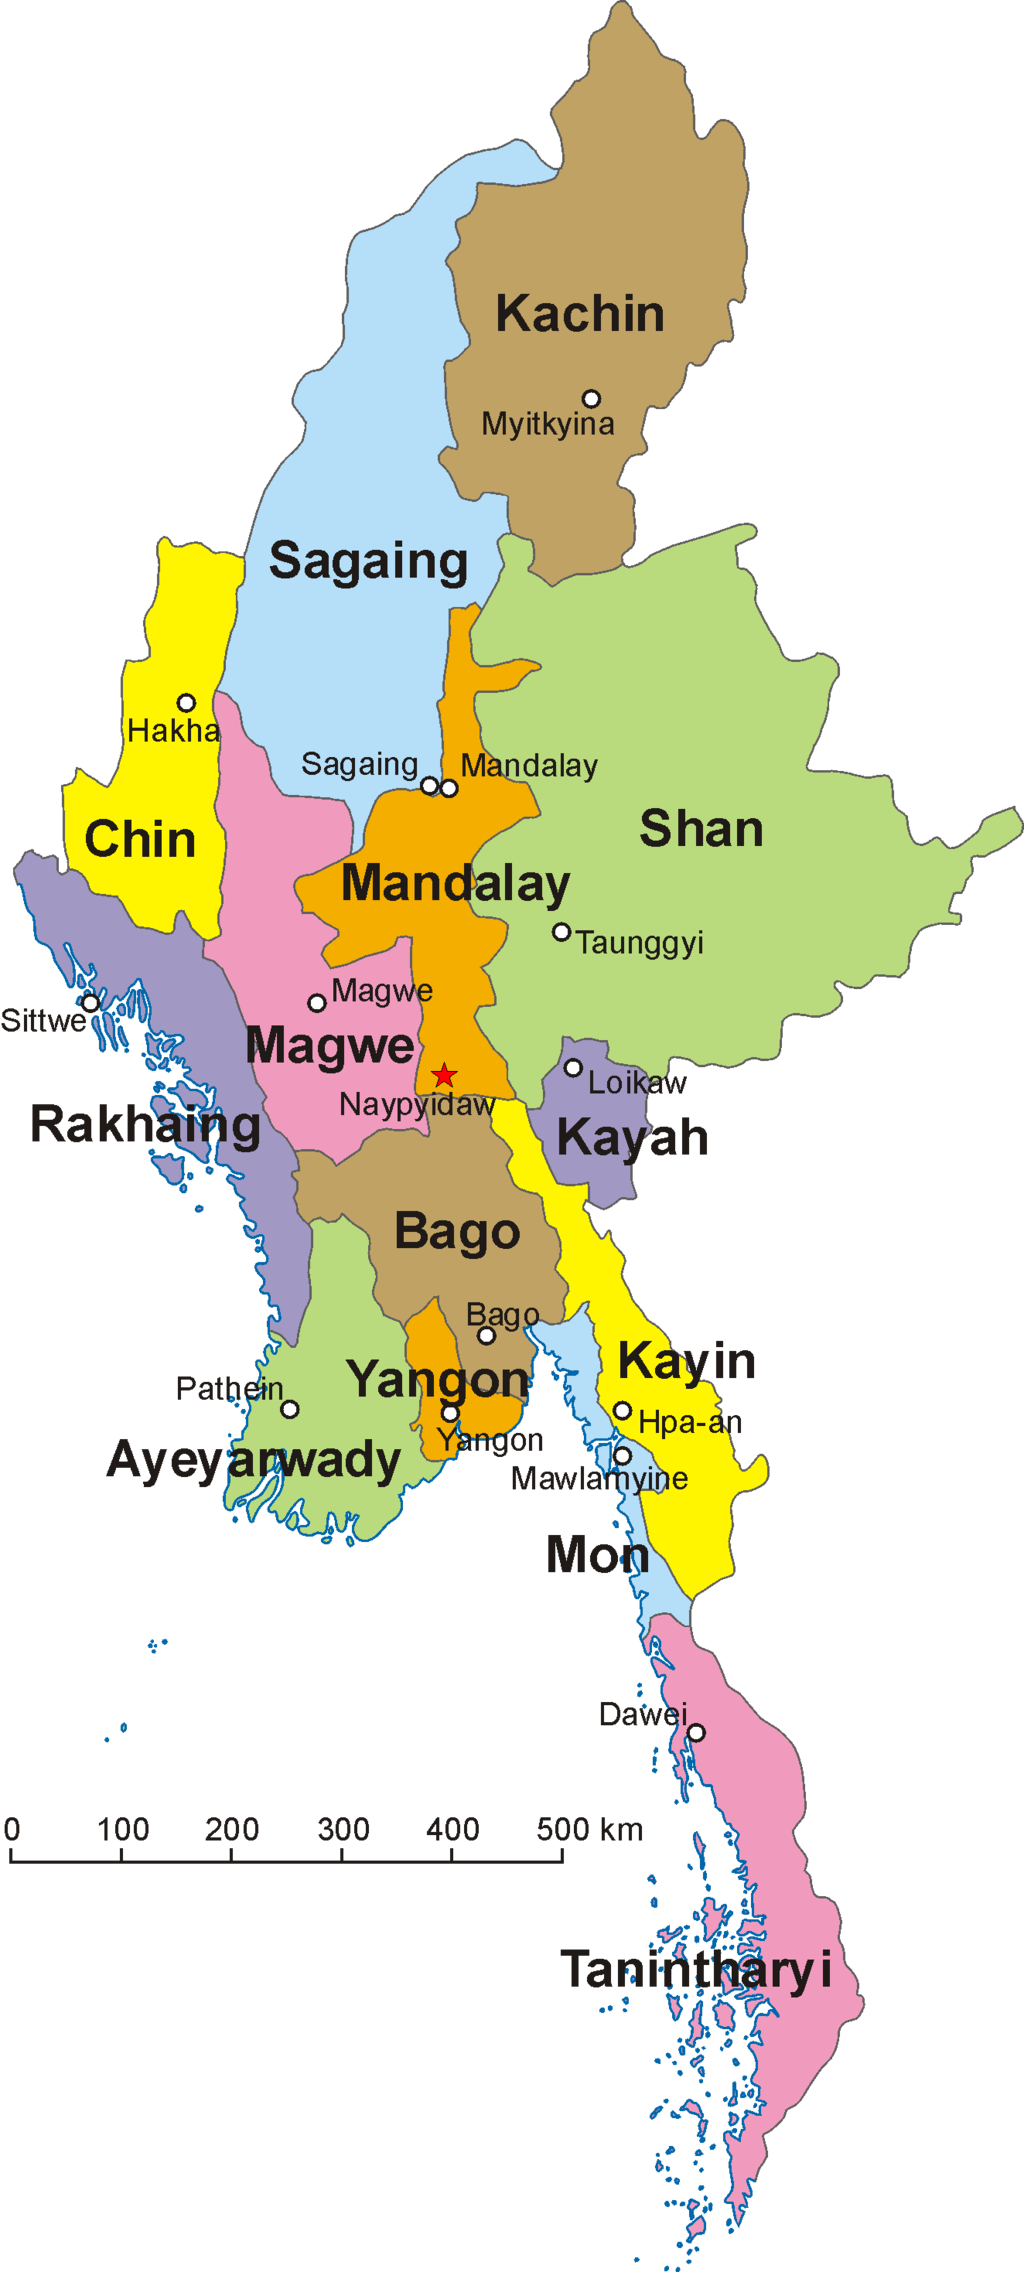
\includegraphics[width=0.5\linewidth]{~/Dropbox/Dissertation/Document/entry_chapter/Burma_en} 

}

\caption{Administrative Districts of Burma. Source: Aotearoa.}\label{fig:burmamap}
\end{figure}

As a whole, Burma is an ethnically diverse society, though ethnic
minorities tend to be concentrated on the largely mountainous periphery
of the country, while ethnic Burmans predominate in the central lowlands
(Steinberg \protect\hyperlink{ref-Steinberg2010}{2010}). In the
pre-colonial era these ethnic identities were relatively fluid, both in
terms of their content and their membership (South
\protect\hyperlink{ref-South2008}{2008}). British colonial rule from
1885--1948 led ethnic categories to become both more calcified and more
salient, as they practiced direct rule over the ethnic Burmans in the
lowlands, while delegating significant autonomy to the ethnic minorities
of the mountainous regions (South
\protect\hyperlink{ref-South2008}{2008}). Furthermore, administrative
practices such as frequent censuses required individuals to declare
their ethnicity (Charney \protect\hyperlink{ref-Charney2009}{2009}), and
most positions in the colonial bureaucracy and security forces were
given to minorities, as the majority Burmans were viewed as a greater
threat to colonial rule (Steinberg
\protect\hyperlink{ref-Steinberg2010}{2010}). Japan occupied Burma
through much of World War II, further entrenching ethnic divisions as
the Burman majority collaborated with the Japanese, while many ethnic
minorities including the Karen and Kachin supported the Allies
(Steinberg \protect\hyperlink{ref-Steinberg2010}{2010}).

Late in the war the most prominent faction of pro-Japanese Burmans, led
by Aung San, switched sides to support Allied efforts to liberate the
country. Most of the politically-active population of Burma, including
most ethnic minorities, joined together to form the Anti-Fascist
People's Freedom League (AFPFL). The organization remained mostly
cohesive for several years after the war in pursuit of independence
(Charney \protect\hyperlink{ref-Charney2009}{2009}). As soon as Aung San
succeeded in negotiating a peaceful conferral of independence from the
British in January 1947, however, ethnic tensions re-emerged. The
Panglong Agreement the following month established the boundaries of the
new Burmese state, placing the minority-dominated Frontier Areas under
Burman control. As several of the minority groups, including the Karen,
had received tacit promises from the British that they would receive
independence as separate states, turmoil ensued (Steinberg
\protect\hyperlink{ref-Steinberg2010}{2010}). Almost immediately upon
gaining independence in 1948, Burma faced two civil wars --- a
secessionist campaign led by the Karen National Union, and a bid to
overthrow the central government by the Red Flag faction of the
Communist Party of Burma.

\hypertarget{the-shan-secessionist-movement}{%
\subsection{The Shan Secessionist
Movement}\label{the-shan-secessionist-movement}}

Shan State is a large, mountainous area in eastern Burma, bordering
Thailand on the south, Laos on the east, and China on the north. The
Shan people and language are both closely related to the Thai, and in
pursuit of its historical rivalry with Burma the Thai government has
frequently supported Shan rebellions to form a sort of buffer zone
between the two countries (Steinberg
\protect\hyperlink{ref-Steinberg2010}{2010}). Adding to the
international character of the region are the facts that it has long
been one of the world's most productive areas for opium cultivation, and
that it was used as refuge by Kuomintang (KMT) forces fleeing China in
the 1950's and 1960's (Cowell \protect\hyperlink{ref-Cowell2005}{2005}).
Shan State initially faced less repression than most other areas of the
country, as it had been granted the right to secede in the Burmese
Constitution (Silverstein
\protect\hyperlink{ref-Silverstein1958}{1958}).

The initial formation of rebellion in Shan State is consistent with the
process of group formation proposed in my theory.\footnote{According to
  the coding rules used in the quantitative analysis, the first Shan
  rebel group initiated the conflict there, rather than joining it.
  However, as there was significant fighting in the area between the
  Burmese government and other non-state actors, I would argue that it
  is consistent with my theory.} Following their defeat in the Chinese
Civil War in 1950, a contingent of KMT soldiers fled into Shan in search
of refuge. During the same period, the Communist Party of Burma and
separatists from the Kachin region frequently used the area as a base of
operations (Smith \protect\hyperlink{ref-Smith1999}{1999}). In hopes of
defeating the Communists and Kachin, and expelling the KMT, the Burmese
army sent a large troop deployment to the region in the late 1950's.
These forces were undisciplined, however, and frequently committed
abuses against the local population (Fredholm
\protect\hyperlink{ref-Fredholm1993}{1993}, 156).

Meanwhile, student groups began developing and promoting Shan
nationalism, including through the dissemination of magazines. The
abuses by the Burmese Army allowed this nationalist movement to gain
traction among the broader population as it became the basis for
opposing the military occupation (Fredholm
\protect\hyperlink{ref-Fredholm1993}{1993}, Ch. 8). The process of
increased ethnic identification in this case is largely consistent with
my theoretical argument. Shan elites, especially the leaders of student
organizations, began developing and advocating for a distinctly Shan
identity in the mid-1950's. Repression by the Burmese army significantly
enhanced the efficacy of these appeals, leading large portions of the
Shan to embrace ethnic nationalism (Fredholm
\protect\hyperlink{ref-Fredholm1993}{1993}, 156--57). In 1958 this
nationalism culminated in the formation of the first Shan rebel group,
the Young Brave Warriors (Lintner
\protect\hyperlink{ref-Lintner1999}{1999}). In theory, Shan dissidents
could have joined the Communist Party of Burma, partnered with the
Kachin Independence Army that often operated in Shan, or perhaps even
partnered with the KMT. Yet as my theory predicts, the chose to form an
explicitly Shan organization.

\hypertarget{the-arakanese-buddhist-rebels}{%
\subsection{The Arakanese Buddhist
Rebels}\label{the-arakanese-buddhist-rebels}}

The Arakan state is located in Western Burma, along its border with
Bangladesh. Today the district is more commonly known as Rakhine state
(or Rakhaing in Figure \ref{fig:burmamap}), and is notable for being the
location of the humanitarian crisis centering around the forced
migration of the Rohingya people. In this case study I will relax the
assumption that different issues of contention constitute entirely
separate conflicts. While the country ultimately saw separatist
movements associated with 11 different territories, the dissident elites
who led these movements were mostly united within the AFPFL prior to
independence. In some cases rebels from different separatist regions
collaborated, even while pursuing different goals (Smith
\protect\hyperlink{ref-Smith1999}{1999}). Furthermore, in some cases
smaller ethnic groups initially participated in the movements of larger
ethnicities, before launching their own rebellion. For example the
Karenni originally participated in the separatist movement of their
relatives the Karen, before later launching their own rebellion (Uppsala
Conflict Data Program \protect\hyperlink{ref-UCDPEncyclopedia}{2016}).
In some cases, then, it might be more accurate to view the new
separatist movements in Burma as having joined a larger ongoing
conflict, rather than initiating an entirely new one. Under this
conception, even the first Arakan separatist groups, the Arakan People's
Liberation Party (APLP) and the Mujahid Party, would be considered as
joining an ongoing conflict in 1948. Even when applying the coding rules
of the quantitative analysis and treating these groups as initiating a
new conflict, two other Buddhist groups clearly qualifier as new groups
--- the Arakan National Liberation Party (ANLP) in 1964, and the Arakan
Liberation Party in 1977.

While Arakan is considered an ethnicity largely because it has a long
history as a unified polity, its residents are divided along religious
lines. Indeed, even in its earliest days (beginning in 1948) the
secessionist movement there was divided into a Muslim faction (the
Mujahid Party) and a Buddhist one (the APLP) (Fredholm
\protect\hyperlink{ref-Fredholm1993}{1993}). This illustrates an
important limitation of my theoretical and empirical approach. I focus
on ethnicity as I expect that it will be the most salient social
cleavage in most countries, because its importance in the context of
civil war has been well-established (see Cederman, Wimmer, and Min
\protect\hyperlink{ref-Cederman2010}{2010}), and because ethnicity is
more easily measured than most other dimensions of identity. Clearly,
however, other cleavages can take priority in some cases, and can
sub-divide ethnicity as is the case in Arakan. Thus, even though both
factions of Arakan residents share a common purpose of securing
independence from Burma, they adopt the potentially counterproductive
arrangement of being organized into separate rebel groups on the basis
of religion.

Ultimately, however, I view the Arakan separatist movement as largely
consistent with my theory. While I expect that repression will
ultimately lead ethnic groups to produce cohesive rebel groups organized
around their identity, and this stops short of occurring in Arakan due
to religious divisions, the reasons why Arakanese organize as they do
are largely consistent with my theory. I expect that individuals will
turn to ethnicity in the face of repression because 1) repression is
often targeted on the basis of ethnicity, increasing the salience of
such groupings, and 2) ethnicity often provides a useful basis for
defense from repression, as ethnic groups often have militias, and may
be able to attract support from co-ethnic outside states.

While Burma was nominally democratic from independence in 1948 until a
military coup in 1962, the quality of human rights in the country was
low. The Latent Human Protection Score for the country was around -1.47
during this period, making it a relatively repressive regime as the
global average over the period was 0.03. For comparison, the score
changed little after what is generally considered to be a very
repressive military regime took power. Thus, at the dawn of the Arakan
independence movement the Burmese government employed a level of
repression that I would expect to provoke increases in the number of
individuals resorting to violence, and to levels of ethnic
identification. But whereas I suspect that repression is generally
targeted disproportionately at certain ethnic groups, in Arakan the
targeting was more specific, with Muslims being disproportionately
targeted relative to Buddhists. In fact, the government renamed the
state ``Rakhine,'' a name that previously referred only to the Buddhist
subset, to emphasize their stance against the Muslim minority known as
the Rohingyas (Fredholm \protect\hyperlink{ref-Fredholm1993}{1993}). The
Burmese government has maintained a military deployment to the region
through much of the conflict, and while it has applied significant
repression to both religions, it has been especially brutal toward the
Rohingya, ultimately seeking to force the minority to migrate into
Bangladesh (Steinberg \protect\hyperlink{ref-Steinberg2010}{2010}).
Thus, the underlying logic of my theory would imply that as repression
is applied with respect to both ethnicity and religion, both dimensions
of identity should be salient.

Once deciding to rebel, it would not be a foregone conclusion that an
Arakanese dissident would choose to form a new rebel group. The
Communist Party of Burma had a strong following in Arakan; joining the
Red Flag faction, or later the Communist Party of Arakan, might have
been a viable option for many. The Karen National Union was also active
prior to any significant military mobilization in Arakan. It is not
obvious, \emph{a priori}, why the various separatists would not band
together, as individually none could pose a serious threat to the
Burmese government. Indeed, most of the separatist movements agreed to
ceasefires in the 1990's and 2000's without winning any concessions, or
coming at all close to military victory. Later in the conflict there
were in fact attempts to build multi-ethnic alliances (Smith
\protect\hyperlink{ref-Smith1999}{1999}). Initially, however, dissidents
generally choose to organize on the basis of ethnicity, in some cases
further subdivided by religion. Geographic isolation surely played some
role in the lack of coordination across regions, but in several cases
separatists operated outside of their own secessionist territory, and
Communist forces frequently traveled between different separatist
regions (Smith \protect\hyperlink{ref-Smith1999}{1999}). Furthermore,
the Arakanese and Karen separatists had been unified under the banner of
the AFLFP just a few months prior, meaning that at least at the elite
level, they had communication channels and a history of interaction. As
Staniland (\protect\hyperlink{ref-Staniland2014}{2014}) notes, social
groups with these sorts of ties are often able to build national rebel
groups. The fact that this did not occur suggests that ethnicity was an
important factor in preventing the consolidation of dissent.

After accounting for the religious cleavage, the organization of
Arakanese rebels is consistent with my expectations. Buddhists and
Muslims generally consolidated into a single rebel group each.
Interestingly, the specific organizations changed over time, with one
group being defeated and another taking its place. For example, when the
Arakan conflict began in 1948, Buddhists were represented by the Arakan
People's Liberation Party. The APLP was defeated in the late 1950's.
Surviving members joined with new recruits to form the Arakan National
Liberation Party a few years later. The ANLP too was defeated, only to
be later replaced by the Arakan Liberation Party. Thus while three new
Buddhist organizations joined the ongoing conflict in Arakan, they
seemingly replaced one another, and represented the same underlying
constituency. This suggests that dissidents only form new organizations
if there is not already a group representing their particular set of
identities. Furthermore, it suggests that there is a persistent demand
for rebel groups to provide representation. If an existing rebel group
is defeated, the potential support of dissident constituents provides an
incentive for entrepreneurs to create a replacement.

Other elements of the Arakan case are broadly consistent with my theory,
while also suggesting nuance. Most of the ethnic minorities faced
significant repression starting almost immediately after World War II,
as the central government sought to create a unified Burmese state. The
Arakanese groups that joined later in the conflict seem to fit my
prediction that repression reduces the disincentive to participate in
violence, though accounts from individual rebels are virtually
non-existent. It should be noted, however, that the initial Arakanese
rebellion, the APLP, was comprised largely of individuals who had fought
the Japanese in World War II (Charney
\protect\hyperlink{ref-Charney2009}{2009}). While the core logic of the
theory likely applies to these individuals --- the brutal Japanese
occupation reduced the relative cost of fighting --- I fail to account
for the fact that conflicts often cluster in space and time, meaning
that the most recent wave of repression will not always be the only
violent experience shaping dissident preferences. The Arakanese also
ultimately formed new rebel groups around the identities that formed the
basis for repression, as I expect. Yet the logic of forming a new group
does not seem to follow the logic I propose. Whereas I expect that new
groups to constitute a rejection of existing rebel groups in response to
their lack of representation for some ethnic groups and inability to
protect civilians, in Arakan the decision was mutual and collaborative.
The Karen National Union was uninterested in recruiting Arakanese
dissidents, but did support the movement and aided in the establishment
of several of the rebel groups there (Smith
\protect\hyperlink{ref-Smith1999}{1999}).

\hypertarget{discussion}{%
\subsection{Discussion}\label{discussion}}

The onset of conflict in Shan State provides an excellent illustration
of my theory. Shan civilians were caught in the crossfire of conflicts
between the Burmese government and two non-state actors, the KMT and the
Kachin Independence Army. The abuses perpetrated against civilians
during this time made them receptive to the nationalist movement being
propagated by Shan elite, facilitating the creation of a distinctly Shan
rebel group. I return to this case in Chapter \ref{realignment}, as it
provides mixed evidence for my predictions regarding splintering and
alliances.

The Arakan case suggests some refinements for my theory, but in most
ways is consistent with its logic. As I predict, the emergence of
rebellion in Arakan followed a period of political and physical
repression, though the residual effects of World War II likely played a
role in producing a pool of individuals wiling to fight. I also expect
that repression will lead individuals to identify more strongly with
their ethnic group. In Arakan state this prediction is not inaccurate,
but is underspecified. The fundamental groups to which Arakanese turned
was a subdivision of their ethnicity that combines ethnic identity with
religion. While I focus on ethnicity for reasons of clarity and data
availability, Arakan shows that a full understanding of any particular
case requires knowledge of the social cleavages there. Identities such
as religion can crosscut ethnicity, and in some cases might even take
priority over it. Indeed a split between Muslims and Christians led to
conflict in the ethnically-homogeneous South Sudan almost immediately
upon its independence. A question raised by this analysis is how rebel
elites are sometimes able to overcome such divisions and produce a
movement that coheres around a broader identity. The Iraqi Kurdish
population, for example, contains Muslims, Christians, and adherents to
a number of smaller religions such as Zoroastrianism. While at times the
Kurds have divided along these lines, they've tended to come together in
the face of conflict (McLauchlin and Pearlman
\protect\hyperlink{ref-McLauchlin2012}{2012}). Future work should
explore why the Kurds have been able to accomplish this, while the
Arakanese have not.

\hypertarget{entry-conclusion}{%
\section{Conclusion}\label{entry-conclusion}}

I have argued that repression should increase the probability that new
rebel groups will join ongoing civil wars. This is so because repression
reduces the relative risk of fighting for previously non-violent
individuals, creating a pool of individuals willing to join the
conflict. Yet because repression also tends to enhance the salience of
ethnic identities, due to the fact such identities often form the basis
for targeting and emphasizing such identities is often a good strategy
for procuring foreign support, these new fighters are not always
interested in joining existing groups. Rather, they should form new
rebel groups that provide explicit representation to their ethnic group.

Consistent with my expectations in \emph{H4}, I find that decreases in
human rights practices are associated with a substantial increase in the
probability that a new rebel group will join the conflict in the
following year. A change of -1 in the Latent Human Protection Score for
a country, roughly the difference between France and Russia in recent
years, triples the probability that a new group will emerge. I do not
find support for \emph{H5}, which predicted that ethnic diversity would
limit the scope in which the repression mechanism should apply. I do
find support for \emph{H6}, which tests the implication that new rebel
groups emerging through this process should be more likely than others
to draw support from a single ethnic group. Rebel groups that join
ongoing conflicts are nearly twice as likely as others to have ties to
only a single ethnic group.

These results suggest that the government plays a surprisingly large
role in shaping rebel movement structure. Existing work on rebel
structure tends to focus on the social (Staniland
\protect\hyperlink{ref-Staniland2014}{2014}) or economic (Weinstein
\protect\hyperlink{ref-Weinstein2007}{2007}) context from which rebels
emerge, and studies that do consider the role of the government have
often found that repression increases cohesion among target groups
(Simmel \protect\hyperlink{ref-Simmel1955}{1955}), though the effect may
be contingent on internal group dynamics (McLauchlin and Pearlman
\protect\hyperlink{ref-McLauchlin2012}{2012}). The findings also
contribute to the school of thought which suggests that ethnic diversity
is not inherently dangerous (Fearon and Laitin
\protect\hyperlink{ref-Fearon1996}{1996}), with ethnic conflict instead
being contingent on the treatment of ethnic groups (Cederman, Wimmer,
and Min \protect\hyperlink{ref-Cederman2010}{2010}). Similarly, these
results suggest that policymakers could limit the emergence of ethnic
polarization during conflicts by ensuring the protection of civilian
populations.

\hypertarget{realignment}{%
\chapter{The Realignment of Rebel Groups}\label{realignment}}

Having explored the formation of new rebel groups in the previous
chapter, I turn now to the other major process affecting the number of
rebel groups in a conflict --- the realignment of existing rebel
factions. There are two ways in which rebels can realign. First, subsets
of existing groups can break away to form splinter organizations. For
example, Hezbollah split from the Amal movement during the Lebanese
Civil War to form a more radical organization. I define a splinter
organization as an independent rebel group, signified by having an
identifiable name and leadership that are not shared with any other
rebel group, that was previously subsumed within another rebel
organization. Thus, entirely new rebel groups are excluded, even if they
constitute a subset of a larger non-violent organization. Splinter
organizations generally emerge during ongoing conflicts, though
sometimes they are formed during periods of peace to initiate a new wave
of fighting, as the Real Irish Republican Army did (Stedman
\protect\hyperlink{ref-Stedman1997}{1997}).

Second, previously independent rebel organizations can form alliances.
Here I focus on alliances with meaningful integration of command
structures, defining an alliance as an organization with a distinct name
that merges a substantial amount of the decision-making for two or more
previously independent rebel groups. This might occur if one group
absorbs another, or two groups create a formal umbrella organization to
coordinate their activities. An example of the latter case is the Syrian
Defense Forces, under which the Kurdish People's Protection Units (YPG)
have joined with several Arab rebel groups to coordinate their campaign
against the Islamic State. Note that this definition excludes
cooperation that falls short of formal integration. Such behavior is
difficult to measure systematically in any case, though multiple
forthcoming data collections should facilitate research on the topic in
the future.

I expect these process to be closely related as part of a broader
process of realignment around ethnic identity. Repression should make
civilians more likely to identify with their ethnic group. While I do
not necessarily expect this effect to extend directly to rebels ---
almost by definition, they experience violence --- I do expect that
there will generally be a strong connection between rebels and civilians
dissidents. Except for a few cases with exceptionally large endowments
of natural resources or foreign support, rebels depend on dissident
civilians for recruits, shelter, and material resources. As civilians
often have the ability to defect to the side of a rival rebel group or
the government, rebels have an incentive to represent the interests and
identities of these constituents. Furthermore, ethnic identification can
be an effective means of securing support from foreign co-ethnic states,
and such appeals might be especially likely to succeed during periods of
repression. Thus, rebels should tend to identify more strongly with
their ethnic group following episodes of repression.

This dynamic should lead rebels to reorganize on the basis of ethnicity.
In some cases rebel leaders may be able to reorient their group to
emphasize ethnicity more strongly (see Christia
\protect\hyperlink{ref-Christia2012}{2012}). Often, however, it will be
difficult for them to do so credibly. For example, if a rebel had
previously maintained a multi-ethnic coalition of support, it would be
difficult for them to emphasize a particular ethnic identity. In such
cases, entrepreneurial members of the group may see opportunities to
form a new splinter organization that ``outbids'' the original rebel
group with a more credible, extreme appeal to ethnic identity (see
Horowitz \protect\hyperlink{ref-horowitz85}{1985}). As doing so could
potentially win the support of a large number of dissident civilians,
and leading a rebel group is likely to bring private benefits such as
resource revenues, this should often be an enticing opportunity. As I
expect this cycle of ethnic outbidding to be especially likely in the
wake of repression, I expect that the level of repression should predict
the likelihood that new splinter organizations will form.

\emph{Hypothesis 6: The probability that rebels groups splinter should
increase with the level of repression in a country}

I argue that splintering often reflects a process of reorganization
around ethnic identity. The ability of this process to produce new rebel
groups should depend, however, on the pre-existing configuration. A
rebel group that is already composed primarily of members of a single
ethnicity may be able to adapt to increased ethnic identification,
though they may still fragment as a result of outbidding appeals.
Nevertheless, groups that draw their support from multiple ethnic groups
should be much more vulnerable to fragmentation as the result of
increased ethnic identification.

\emph{Hypothesis 7: Multi-ethnic rebel groups should be at greater risk
of splintering than mono-ethnic ones}

My theory also suggests a testable implication regarding the
characteristics of the splinters groups that emerge. If splintering is
motivated by a desire to form rebel groups that more clearly represent a
particular ethnic group, the rebel groups that emerge from this process
should be likelier than others to draw their support from a single
ethnic group.

\emph{Hypothesis 8: Splinter organizations should be more likely than
others to draw their support from a single ethnic group}

While this process of realignment around ethnic identities should lead
to the fragmentation of some groups, in other cases it might create
opportunities for aggregation. One disadvantage of splintering is that
it will generally result in a weaker organization than members had
previously, as it will have only a subset of the parent group's members
at its disposal. As a crucial function of alliances is the aggregation
of capabilities, forming new alliances is a potential solution to this
problem. Alliances may also have the benefit of managing potential
conflict between their members (Gibler
\protect\hyperlink{ref-Gibler1996}{1996}), ensuring that resources are
directed toward fighting the government rather than other rebel groups.
Finally, outside states often attempt to maximize the impact of their
support by channeling it to a coalition of rebels, rather than a series
of smaller, independent groups. Interventions of this sort might be
especially likely in the wake of a humanitarian crisis.

As is the case with splintering, my theory offers predictions regarding
not only when new alliances should emerge, but also what their ethnic
composition should be. I expect that the ethnic polarization sparked by
repression should lead rebels to leave multi-ethnic coalitions, but also
to form new alliances with co-ethnic factions.

\emph{Hypothesis 9: The probability that new mono-ethnic alliances will
form should increase with the level of repression}

Conversely, the emergence of multi-ethnic alliances should be less
likely when this dynamic is at work.

\emph{Hypothesis 10: The probability that new multi-ethnic alliances
will form should decrease with the level of repression}

I proceed with an explanation for a research design for these four
hypotheses. After presenting the findings, I assess the effect of
repression on the total number of rebel groups.

\hypertarget{research-design-2}{%
\section{Research Design}\label{research-design-2}}

While I believe them to be the result of closely related theoretical
processes, the splintering of individual rebel organizations and the
formation of alliances between separate organizations require distinct
research designs. This is so because the unit of analysis in the
splintering study is the rebel group-year, whereas alliance formation is
a decision by multiple rebel groups, and thus the unit of analysis is
the conflict-year. I first explain the research design for splintering
in greater detail, before explaining the differences in the alliance
formation design.

\hypertarget{splintering-2}{%
\subsection{Splintering}\label{splintering-2}}

The first phenomenon I explain in this chapter is splintering. As the
explanatory factors in \emph{H7} and \emph{H8} are group attributes, the
unit of analysis in this portion of the study is the rebel group-year. I
seek to explain not simply which conflict years produce splinter
organizations, but also which rebel groups within those conflict years.
I draw my sample of cases from the UCDP Dyadic Dataset, version 4-2016
(Melander, Pettersson, and Themnér
\protect\hyperlink{ref-Melander2016}{2016}), which includes an
observation for every non-state actor in every year in which it was
involved in conflict with the government producing at least 25
fatalities. After collapsing observations for rebel groups that appear
in multiple conflicts in a single year, I am left with a dataset of
2,656 rebel group years covering the period 1946--2015.

\hypertarget{dependent-variables-2}{%
\subsubsection*{Dependent Variables}\label{dependent-variables-2}}
\addcontentsline{toc}{subsubsection}{Dependent Variables}

\textbf{Splintering}

The first dependent variable in this portion of the analysis is the
splintering of existing rebel groups. I use my own data on rebel group
origins to identify splinter groups.\footnote{The UCDP Actor data
  (Uppsala Conflict Data Program
  \protect\hyperlink{ref-ucdpactor}{2015}) does identify splinter
  groups, but uses very conservative coding rules that exclude many
  clear examples of splinter.} A group is coded as a splinter
organization if most of its leadership were previously members of
another rebel group. I follow the UCDP coding decisions for
distinguishing cases where a new group has emerged from simple name
changes. Essentially, a group is considered new if its leadership,
organizational structure, or membership differs substantially from
previous existing organizations. When two groups disagree about which is
the original organization and which is the splinter, the larger group is
considered the original.

113 of the 506 rebel groups in my data are splinter organizations. As
there are four cases in which a rebel group produced two splinter
organizations in the same year, the number of years in which a new
splinter organization emerged is 109. However, a large portion of these
are coterminous with dissolution of the original organization. Typically
in these cases the main organization will agree to a peace deal, and a
radical faction will form a splinter organization to continue fighting.
While this is an interesting and consequential phenomenon, it has
already received a substantial amount of attention from scholars (e.g.
Stedman \protect\hyperlink{ref-Stedman1997}{1997}). Though empirically
they may overlap in some cases, the division between hardliners and
moderates is analytically distinct from ethnic divisions, suggesting it
is a separate process from what I theorize. Furthermore, I am interested
in processes that increase or decrease the number of rebel groups in a
conflict. Replacing a large, moderate organization with a more radical
splinter has important implications for the probability of peace and the
tactics likely to be deployed. Ultimately, however, it does not alter
the number of rebel groups competing simultaneously. I thus consider
these cases to be beyond the scope of this dissertation, and exclude
them from my analyses. This leaves a total of 25 cases in which a
splinter and parent organization were active simultaneously. This
variable is coded as 1 in the group-year in which a parent organization
loses a splinter faction (i.e.~I examine the groups that splinter).

\textbf{Rebel Group Ethnicity}

\emph{H8} predicts that splinter organizations should be more likely
than others to draw support from a single ethnic group. As I did for the
similar hypothesis in Chapter \ref{entry}, I use the the ACD2EPR 2014
dataset (Wucherpfennig et al.
\protect\hyperlink{ref-Wucherpfennig2011}{2011}; Vogt et al.
\protect\hyperlink{ref-Vogt2015}{2015}) to determine this. The data
measures three categories of ties between rebel and ethnic groups ---
explicit claims of representation, recruiting, and support from at least
half the ethnic group. I collapse these forms to code a trichotomous
measure indicating whether a rebel group is multi-ethnic, mono-ethnic,
or non-ethnic, meaning it has no observable links to any ethnic group.

\hypertarget{independent-variables-2}{%
\subsubsection*{Independent Variables}\label{independent-variables-2}}
\addcontentsline{toc}{subsubsection}{Independent Variables}

\textbf{Human Rights}

I again use the Latent Human Protection scores, version 2 (Fariss
\protect\hyperlink{ref-Fariss2014}{2014}; Schnakenberg and Fariss
\protect\hyperlink{ref-Schnakenberg2014}{2014}) to measure repression.
As I do in Chapter \ref{entry}, I combat the fact that the measure is
mostly static with a slight positive trend over time by using the change
over the previous. In this measure, a negative score indicates that a
country has become more repressive, while a positive score means that
human rights have improved. In this sample the mean change is just 0.01,
but there are numerous large change in both directions.

\textbf{Multi-ethnic Group}

To test \emph{H7} I use the measure of rebel group ethnicity that serves
as a dependent variable later in the chapter. In this case I collapse
the measure into a dichotomous indicator with rebel groups that draw
support from multiple ethnic groups coded as 1, and all others coded as
zero. There are relatively few multi-ethnic groups in the data, with the
attribute occurring in 334 of 2393 valid group-year observations.

\textbf{Splinter Organization}

The test of \emph{H8} uses the splinter variable from my rebel origins
data as an explanatory factor. The coding rules are described above. 113
out of 503 rebel groups are splinter organizations.

\hypertarget{control-variables-2}{%
\subsubsection*{Control Variables}\label{control-variables-2}}
\addcontentsline{toc}{subsubsection}{Control Variables}

I include many of the country-level covariates from Chapter \ref{entry}
in the splintering analyses as controls. These include ethnolinguistic
fractionalization (Fearon and Laitin
\protect\hyperlink{ref-fearonlaitin03}{2003}), Polity IV score
(Marshall, Gurr, and Jaggers
\protect\hyperlink{ref-Marshall2016}{2016}), land area (The World Bank
\protect\hyperlink{ref-WorldBank2015}{2015}), population (Gleditsch
\protect\hyperlink{ref-Gleditsch2002b}{2002}), GDP per capita (Gleditsch
\protect\hyperlink{ref-Gleditsch2002b}{2002}), and a count of lootable
resource sites (Lujala, Rød, and Thieme
\protect\hyperlink{ref-Lujala2007}{2007}; Gilmore et al.
\protect\hyperlink{ref-Gilmore2007}{2005}; Lujala, Gleditsch, and
Gilmore \protect\hyperlink{ref-Lujala2005}{2005}; Balestri
\protect\hyperlink{ref-Balestri2012}{2012}; Lujala
\protect\hyperlink{ref-Lujala2008}{2008}; Buhaug and Lujala
\protect\hyperlink{ref-Buhaug2005}{2005}). Refer to the previous chapter
for detailed descriptions.

Additionally I include several rebel group-level controls from
Cunningham, Gleditsch, and Salehyan
(\protect\hyperlink{ref-Cunningham2009}{2009}). These include a binary
indicators of whether the rebel group is stronger than the government,
whether the group has a presence in multiple states, whether the group
has a political wing, whether the group controls territory, whether the
group has centralized control, and whether it receives external support.
Each of these measures is a snapshot, measured for each group at only
one point in time.

\hypertarget{modeling-strategies}{%
\subsubsection*{Modeling Strategies}\label{modeling-strategies}}
\addcontentsline{toc}{subsubsection}{Modeling Strategies}

To test \emph{H6} and \emph{H7} I use a Cox proportional hazard survival
model. This is a useful modeling framework in this case because the
probability that a rebel group will splinter is in part a function of
time. In a standard logistic regression analysis with the rebel group as
the unit of analysis, the duration of time the group was active is such
a strong predictor of splintering that it typically nullifies the
significance of all other variables. Survival models address this by
treating splintering as a function of time, expressed as the probability
that a rebel group will survive a given number of years without
splintering. Independent variables explain deviations from this baseline
survival curve. The Cox model is likely to be the proper choice of
survival models in this case, as survival times for rebel groups are
heavily right-skewed, and the Cox model does not assume survival times
form any particular distribution (i.e.~it is non-parametric).

The exact specification of the dependent variable in this analysis is
the number of years between a rebel group's first appearance in the data
and the first time it generates a splinter organization. I remove a
rebel group from the study once it has splintered for the first time.
This results in the exclusion of three instances of splintering from
rebel groups that had splintered previously. As many of my covariates
are measured at the country level and there are often multiple rebel
groups per country, I cluster the standard errors by country.

To test \emph{H8} I use a simple logistic regression with the rebel
group as the unit of analysis. The mono-ethnic indicator is the
dependent variable, and the indicator of whether the group is a splinter
organization is the main predictor.

\hypertarget{alliance-formation-2}{%
\subsection{Alliance Formation}\label{alliance-formation-2}}

The research design for the two alliance formation hypotheses (\emph{H9}
and \emph{H10}) closely resembles the group formation analysis from
Chapter \ref{entry}. The unit of analysis is the conflict-year. While I
control for the number of rebel groups, I do not exclude observations
that have only one rebel group. There are several cases where a new
rebel group enters a conflict and joins an alliance in the same calendar
year.

\hypertarget{dependent-variable}{%
\subsubsection*{Dependent Variable}\label{dependent-variable}}
\addcontentsline{toc}{subsubsection}{Dependent Variable}

The dependent variables for the two hypotheses are the formation of two
different types of alliances --- mono-ethnic and multi-ethnic. I use my
data on rebel origins to determine when a new alliance has formed. I
code an alliance as any group whose members are drawn from at least two
distinct previously active rebel groups. These alliances constitute a
substantial enough integration of command that they replace their
constituent groups in the data. In many cases, however, the alliance
splinters and the members groups re-enter the data. I combine the
alliance measure with the ethnic composition variable to code two
dependent variables --- the formation of new multi-ethnic alliances, and
of new mono-ethnic ones. Alliances involving this degree of integration
are rare. New mono-ethnic alliances form in 29 of 2014 conflict-years,
while there are only 13 years in which a new multi-ethnic alliance
emerged.

\hypertarget{independent-variable}{%
\subsubsection*{Independent Variable}\label{independent-variable}}
\addcontentsline{toc}{subsubsection}{Independent Variable}

I use same measure of human rights as in the preceding analyses. I again
use the lagged change in the Latent Human Protection Score (Fariss
\protect\hyperlink{ref-Fariss2014}{2014}; Schnakenberg and Fariss
\protect\hyperlink{ref-Schnakenberg2014}{2014}). The mean change in this
data is -0.01, with a range from -2.51 to 1.50.

\hypertarget{control-variables-3}{%
\subsubsection*{Control Variables}\label{control-variables-3}}
\addcontentsline{toc}{subsubsection}{Control Variables}

I include two conflict-level controls: a binary indicator of whether the
conflict produced 1,000 or more fatalities in a year, and a binary
indicator of whether multiple rebel groups participated in the conflict
in a year. Both measures come from the UCDP Dyadic Data (Melander,
Pettersson, and Themnér \protect\hyperlink{ref-Melander2016}{2016}).
Additionally I control for several country-level factors, including
ethnolinguistic fractionalization and the percentage of terrain that is
mountainous (Fearon and Laitin
\protect\hyperlink{ref-fearonlaitin03}{2003}), population and GDP per
capita (Gleditsch \protect\hyperlink{ref-Gleditsch2002b}{2002}), the
Polity IV score (Marshall, Gurr, and Jaggers
\protect\hyperlink{ref-Marshall2016}{2016}), and an indicator of whether
there was a civil war in a neighboring country.

\hypertarget{modeling-strategy}{%
\subsubsection*{Modeling Strategy}\label{modeling-strategy}}
\addcontentsline{toc}{subsubsection}{Modeling Strategy}

As both dependent variables are binary but rare, I use a logistic
regression with a rare events correction (King and Zeng
\protect\hyperlink{ref-King2001a}{2001}). As there are sometimes
multiple conflicts in a country-year, I cluster the standard errors by
country.

\hypertarget{splintering-results}{%
\section{Splintering Results}\label{splintering-results}}

Results of the splintering analysis are reported in Table
\ref{tab:survival}. I fit five Cox proportional hazard models with
different batteries of covariates. Model 1 includes only the two
independent variables used to test my hypotheses --- the lagged change
in human rights, and an indicator of whether the rebel group is
multi-ethnic. In Model 2 I add several country-level control variables.
Model 3 combines the change in human rights with a set of rebel
group-level controls.

\begin{table}
\begin{center}
\begin{tabular}{l c c c }
\hline
 & Model 1 & Model 2 & Model 3 \\
\hline
Change in Human Rights            & $-1.23^{\dagger}$ & $-1.34$  & $-1.35^{\dagger}$ \\
                                  & $(0.74)$          & $(0.94)$ & $(0.81)$          \\
Multi-ethnic Group                & $0.54$            & $-0.14$  & $0.55$            \\
                                  & $(0.65)$          & $(1.01)$ & $(0.54)$          \\
Polity                            &                   & $-0.02$  &                   \\
                                  &                   & $(0.05)$ &                   \\
Logged GDPpc                      &                   & $0.17$   &                   \\
                                  &                   & $(0.36)$ &                   \\
Logged Population                 &                   & $-0.44$  &                   \\
                                  &                   & $(0.30)$ &                   \\
Logged Area                       &                   & $0.08$   &                   \\
                                  &                   & $(0.40)$ &                   \\
Ethnolinguistic Fractionalization &                   & $0.85$   &                   \\
                                  &                   & $(1.16)$ &                   \\
Lootable Resource Sites           &                   & $0.01$   &                   \\
                                  &                   & $(0.01)$ &                   \\
Intensity Level                   &                   & $-1.34$  &                   \\
                                  &                   & $(1.06)$ &                   \\
Transnational Group               &                   &          & $0.39$            \\
                                  &                   &          & $(0.87)$          \\
Political Wing                    &                   &          & $-0.56$           \\
                                  &                   &          & $(0.46)$          \\
Stronger than Gov.                &                   &          & $2.05^{*}$        \\
                                  &                   &          & $(0.92)$          \\
\hline
AIC                               & 171.59            & 101.72   & 145.35            \\
R$^2$                             & 0.00              & 0.00     & 0.00              \\
Max. R$^2$                        & 0.09              & 0.06     & 0.08              \\
Num. events                       & 20                & 12       & 17                \\
Num. obs.                         & 1908              & 1499     & 1740              \\
Missings                          & 749               & 1158     & 917               \\
PH test                           & 0.06              & 0.59     & 0.74              \\
\hline
\multicolumn{4}{l}{\scriptsize{$^{***}p<0.001$, $^{**}p<0.01$, $^*p<0.05$, $^{\dagger}p<0.1$}}
\end{tabular}
\caption{Cox Proportional Hazard Models of Rebel Group Splintering}
\label{tab:survival}
\end{center}
\end{table}

The coefficients of a Cox model represent the effect of a variable on
the hazard of failure (splintering in this case). A positive coefficient
indicates that the risk of splintering increases with the level of that
variable, while a negative coefficients signifies a reduced risk.
Consistent with \emph{H6} I find that the change in human rights is
negatively related to the hazard of splintering. As human rights improve
the risk that a rebel group will splinter decreases; as a country
becomes more repressive, the risk of splintering increases. However, the
effect is only statistically significant in Models 1 and 4, and even
then only at the 90\% level. The effect size is large, with a one-unit
increase in human rights being associated with a 70\% reduction in the
likelihood of splintering in Model 1, and a 74\% reduction in Model 4.
The relationship is not significant in Model 2, though it is not clear
whether the relationship is confounded by the country-level covariates,
or the change is the result of missing data on those variables.

The findings are thus mostly consistent with \emph{H6}, though not as
robust as most of the analyses in the preceding chapters. Several cases
from the data clearly fit my theoretical framework. The Karenni ethnic
group of Burma are close relatives of the Karen, and fought as members
of the Karen National Union (KNU) for the first several years of Burmese
independence. In 1957, however, the Karenni left the KNU to form their
own rebel group, the Karenni National Progressive Party (KNPP). This
case illustrates that splintering does not always lead to hostile
relations between the formerly united groups, however, as the KNU
strongly supported the KNPP's desire to pursue a separate Karenni state
(Fredholm \protect\hyperlink{ref-Fredholm1993}{1993}). The Free Aceh
Movement splintered from Darul Islam in Indonesia to pursue independence
for the Acehnese people, rather than the Darul Islam's goals of an
Islamic State in Indonesia. A review of the cases also suggests a
possible explanation for the lack of robustness --- communist rebel
groups are highly prone to fragmentation, and account for a large
portion of the splinter organizations.

I find no support for \emph{H7}, as the multi-ethnic variable never
approaches statistical significance. As I discuss in the study of the
Shan State independence movement later in this chapter, it is seemingly
common for ethnically homogeneous groups to splinter. Only one control
variable is significant --- the indicator of whether a rebel group is
stronger than the government in Model 3. Being stronger than the
government increases the risk of splintering by a factor of seven. This
suggests that splintering has a strong strategic element. When rebels
are weak and cannot afford any loss in capability, they hang together.
When victory appears likely, however, they act on their internal
differences, perhaps with an eye toward post-war bargaining.

Disaggregating the sample by conflict type reveals that the findings are
driven largely by secessionist conflicts (see Tables
\ref{tab:survival-govt} and \ref{tab:survival-sec} in the Chapter 5
Appendix). As is the case in the full sample, worse human rights
practices are associated with an enhanced probability of splintering
among secessionist conflicts in Models 1 and 3. Among conflicts for
control of the central government, the relationship is not significant
except in Model 2. This result should be interpreted with caution,
however, as missing data leaves only four instances of splintering in
this model. These results are perhaps not entirely consistent with my
theory. Whereas I expect that splintering to be driven by a process of
realignment around ethnic identity. While splintering is slightly more
common among rebellions against the central government, the phenomenon
is more closely related to repression among secessionist rebellions. It
may be the case that these secessionist movements are realigning around
an identity more specific than ethnicity, such as a particular
combination of religion and ethnicity. Indeed, this pattern can be
observed in several of the secessionist movements in Burma. It is also
possible, however, that the activation of sub-national identities by
repression is not a common pathway to splintering.

In summary the results of this analysis are largely consistent with my
broader theory, though not robust to the inclusion of country-level
controls. I interpret the results as suggesting that ethnic polarization
is a common pathway to splintering. It is not, however, the only
pathway. Communist rebellions are prone to splintering along doctrinal
lines, and splinter organizations often emerge late in conflicts to
continue the fighting after the original organization ceases its
activities.

\hypertarget{splinter-group-ethnicity}{%
\subsection{Splinter Group Ethnicity}\label{splinter-group-ethnicity}}

\emph{H8} predicts that splinter organizations should be more likely
than others to draw their support from a single ethnic group. If
splintering is fundamentally about reorganization along ethnic lines, it
stands to reason that the leaders of splinter organizations should take
only co-ethnics with them. I test this proposition in Table
\ref{tab:splintcomp}. I do not find support for \emph{H8}, as splinter
organizations are not likely than others (alliances and originating
rebel groups constitute the baseline) to be ethnically-homogeneous.
Splinter organizations also do not significantly differ in their
probability of being multi-ethnic. I do find that splinter organizations
are less likely less likely than others to have no ties to any ethnic
group, with the effect being significant at the 95\% level. This
suggests that support from ethnic constituents might be an important
factor in facilitating splintering. Factions that lack such support may
be more likely to remain in the original rebel group, as they have less
assurance of being able to acquire enough resources to be a viable
independent group. The results are not significant when looking at
secessionist and government conflicts in isolation, though this may be a
reflection of the reduced sample size (see Tables
\ref{tab:splintcomp-gov} and \ref{tab:splintcomp-sec} in the Chapter 5
Appendix).

\begin{table}
\begin{center}
\begin{tabular}{l c c c }
\hline
 & M4 Monoethnic & M5 Multiethnic & M6 Nonethnic \\
\hline
(Intercept)                      & $0.20$       & $-3.70^{***}$ & $-0.04$     \\
                                 & $(0.29)$     & $(0.63)$      & $(0.31)$    \\
Splinter                         & $0.39$       & $0.54$        & $-1.14^{*}$ \\
                                 & $(0.41)$     & $(0.54)$      & $(0.57)$    \\
Joiner                           & $0.75^{*}$   & $-1.08$       & $-0.47$     \\
                                 & $(0.34)$     & $(0.66)$      & $(0.37)$    \\
Secessionist                     & $1.07^{***}$ & $-1.18^{*}$   & $-0.76^{*}$ \\
                                 & $(0.31)$     & $(0.50)$      & $(0.36)$    \\
Previously Active                & $-0.08$      & $0.04$        & $0.17$      \\
                                 & $(0.42)$     & $(0.58)$      & $(0.52)$    \\
Ethnlinguistic Fractionalization & $0.16$       & $2.09^{*}$    & $-1.15^{*}$ \\
                                 & $(0.45)$     & $(0.85)$      & $(0.52)$    \\
Transnational                    & $0.06$       & $1.06^{*}$    & $-0.69^{*}$ \\
                                 & $(0.26)$     & $(0.42)$      & $(0.31)$    \\
\hline
AIC                              & 393.19       & 193.69        & 320.15      \\
BIC                              & 419.59       & 220.09        & 346.55      \\
Log Likelihood                   & -189.60      & -89.85        & -153.07     \\
Deviance                         & 379.19       & 179.69        & 306.15      \\
Num. obs.                        & 321          & 321           & 321         \\
\hline
\multicolumn{4}{l}{\scriptsize{$^{***}p<0.001$, $^{**}p<0.01$, $^*p<0.05$}}
\end{tabular}
\caption{Logit Models of Rebel Group Ethnic Composition}
\label{tab:splintcomp}
\end{center}
\end{table}

\hypertarget{alliance-formation-results}{%
\section{Alliance Formation Results}\label{alliance-formation-results}}

The alliance formation results are reported in Table \ref{tab:alliance}.
Model 4 uses mono-ethnic alliances as the dependent variable, while
Model 5 focuses on multi-ethnic alliances and Model 6 combines all
alliances. In \emph{H9} I predict that the probability of new ethnically
homogeneous alliance will be greater following increases in repression.
Consistent with this prediction, the ``Change in Human Rights'' variable
has a strong negative relationship with the probability of new rebel
group formation. A one-unit decrease in human rights (again, roughly the
difference between France and Russia in recent years) more than triples
the odds of a new rebel group forming. In the years following the
largest declines in human rights practices (-2.5), the probability of a
new mono-ethnic alliance is 0.21 (see Figure \ref{fig:zeligplot}). When
the change is zero or positive, the probability of such an alliance is
around 0.01. This relationship is statistically significant at the 90\%
level. Given that the sample size is not especially small (n=1209), an
\(\alpha\) of 0.1 might be considered overly permissive. However, no
other variable is significant at even the 90\% level, suggesting that
even after applying the rare events correction the model has limited
statistical power. Thus, I contend that it is reasonable to interpret
relationships at this significance level, and reject the null hypothesis
of no relationship between repression and the emergence of mono-ethnic
rebel groups.

\begin{table}
\begin{center}
\begin{tabular}{l c c c }
\hline
 & M4 Mono-ethnic & M5 Multi-ethnic & M6 All \\
\hline
(Intercept)                       & $1.56$            & $-1.25$   & $1.71$            \\
                                  & $(3.82)$          & $(12.46)$ & $(2.84)$          \\
Change in Human Rights            & $-1.20^{\dagger}$ & $-1.15$   & $-0.99^{\dagger}$ \\
                                  & $(0.70)$          & $(1.26)$  & $(0.55)$          \\
Ethnolinguistic Fractionalization & $0.79$            & $11.27$   & $1.12$            \\
                                  & $(1.21)$          & $(10.54)$ & $(0.95)$          \\
Intensity Level                   & $0.09$            & $0.54$    & $0.03$            \\
                                  & $(0.58)$          & $(0.89)$  & $(0.45)$          \\
Prev. Multi-rebel                 & $-0.42$           & $0.35$    & $0.31$            \\
                                  & $(0.78)$          & $(0.88)$  & $(0.47)$          \\
Contiguous Civil War              & $0.01$            & $0.08$    & $-0.06$           \\
                                  & $(0.15)$          & $(0.28)$  & $(0.13)$          \\
Logged GDP per capita             & $-0.39$           & $-0.78$   & $-0.43^{\dagger}$ \\
                                  & $(0.35)$          & $(1.01)$  & $(0.26)$          \\
Logged Population                 & $-0.33$           & $-0.75$   & $-0.29$           \\
                                  & $(0.26)$          & $(0.70)$  & $(0.20)$          \\
Polity                            & $-0.04$           & $0.00$    & $-0.01$           \\
                                  & $(0.05)$          & $(0.11)$  & $(0.04)$          \\
\hline
AIC                               & 163.10            & 71.96     & 241.14            \\
BIC                               & 214.07            & 122.94    & 292.12            \\
Log Likelihood                    & -71.55            & -25.98    & -110.57           \\
Deviance                          & 143.10            & 51.96     & 221.14            \\
Num. obs.                         & 1209              & 1210      & 1210              \\
\hline
\multicolumn{4}{l}{\scriptsize{$^{***}p<0.001$, $^{**}p<0.01$, $^*p<0.05$, $^{\dagger}p<0.1$}}
\end{tabular}
\caption{Rare Events Logit Models of Alliance Formation}
\label{tab:alliance}
\end{center}
\end{table}

In Model 5 I do not find support for \emph{H10}, as the relationship
between ``Change in Human Rights'' and the probability of new
multi-ethnic alliances does not approach statistical significance. While
repression does not seem to deter this type of alliance as I expected,
neither does it make them more likely. Thus while I find that repression
is associated with a general increase in the probability of new
alliances, the relationship seems to be driven by ethnically-homogeneous
coalitions. The effect of repression seems to be specific to this type
of alliance, rather than producing a general increase in the propensity
to form coalitions. Disaggregating the results by conflict intensity
reveals that the findings are primarily driven by less severe conflicts,
as the results hold for conflict-years with fewer than 1,000 fatalities,
but not for those with greater than 1,000 (see Tables
\ref{tab:alliance-conflict} and \ref{tab:alliance-war} in the Chapter 5
Appendix). The result for mono-ethnic alliances holds among conflicts
over the central government, but not among secessionist conflicts. The
combined alliance formation result holds in neither subsample (see
Tables \ref{tab:alliance-gov} and \ref{tab:alliance-sec}). As is the
case in previous analyses, my hypotheses perform best in lower-intensity
government conflicts. One explanation for the intensity result is that
forming alliances requires an opportunity for rebel elites to meet and
negotiate a merger, which is unlikely to occur during periods of intense
fighting. The conflict type results again suggests that secessionist
movements tend to be unified around ethnic identity from the outset, and
thus have less need to engage in realignment.

\begin{figure}
\centering
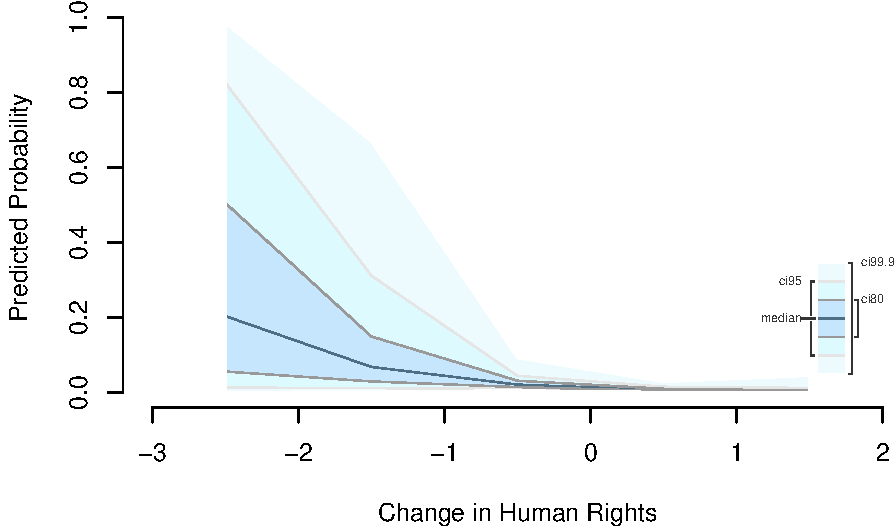
\includegraphics{dissertation_files/figure-latex/zeligplot-1.pdf}
\caption{\label{fig:zeligplot}Predicted Probability of Mono-ethnic Alliance
(Model 1)}
\end{figure}

The only statistically significant control variable in any of the three
models is logged GDP per capita in Model 3. The relationship is
negative, indicating that alliances are less common in wealthier
countries. One possible explanation is that the variable is acting as a
proxy for the intensity or spread of the conflict, capturing an
attribute distinct from the binary measure of whether the conflict
produced 1,000 fatalities. In cases such as Afghanistan where most of
the country is consumed by war, the economy is likely to suffer. In
cases where the fighting is more localized, such as Ukraine in recent
years, there will not necessarily be a significant economic decline at
the country level. The former situation might be more likely to have a
plethora of rebel groups available to form alliances.

The findings in this section are broadly consistent with my theoretical
framework. Increased repression is associated with higher probabilities
of the formation of ethnically homogeneous alliances, which supports my
expectation that repression triggers a cycle of realignment around
ethnic identity. One case that is consistent with this story is the
Uganda National Liberation Front. Uganda is among the most ethnically
diverse societies on earth, with an ethnolinguistic fractionalization
score indicating that there is nearly a 90\% chance that two randomly
selected individuals will be from different ethnic groups. A number of
small rebel groups formed there in 1978 with the goal of overthrowing
Idi Amin, to which the government responded with a substantial increase
in repression (a change of -0.5 in the Latent Human Protection Scores).
In early 1979, with help from the Tanzanian government, several
ethnically Lango rebel groups responded by a forming an alliance, the
Uganda National Liberation Front. A month later they successfully
overthrew Amin. While numerous small rebel groups were active during
this time (Lewis \protect\hyperlink{ref-Lewis2016}{2016}), only the bloc
of Lango groups was able to successfully form an alliance.

\hypertarget{combining-the-processes}{%
\section{Combining the Processes}\label{combining-the-processes}}

This project is motivated by a desire to explain variation in the number
of rebel groups across and within conflicts. To this point, I have
examined individually three processes that increase or decrease the
number of rebel groups. Doing this has allowed me to discuss very
specific causal processes. Yet examining each process separately does
not allow me to speak to the total number of rebel groups we should
expect at various levels of repression. It is not clear, for example, to
what extent alliances offset the increases to the number of rebel groups
brought by splintering. As a final quantitative analysis, I combine
group formation, splintering, and alliance formation and model the
probability that there will be multiple rebel groups active in a
conflict-year. To do this I fit a logistic regression model with a
binary indicator of whether there were at least two rebel groups present
in a conflict year.\footnote{A count model such as Poisson regression
  would not be appropriate here, as rebel groups can persist across time
  periods, violating the assumption of independent counts in each
  period.} The unit of analysis is again the conflict-year, and the
controls are each described in the research design for the alliance
analysis.

\begin{table}
\begin{center}
\begin{tabular}{l c c c }
\hline
 & M7 & M8 & M9 \\
\hline
(Intercept)                             & $-2.25$      & $-1.93$       & $-2.05$       \\
                                        & $(1.48)$     & $(1.50)$      & $(1.44)$      \\
Change in Human Rights                  & $-1.04^{**}$ & $-1.06^{**}$  &               \\
                                        & $(0.39)$     & $(0.39)$      &               \\
Human Rights                            &              &               & $-0.77^{***}$ \\
                                        &              &               & $(0.19)$      \\
Ethnolinguistic Fractionalization       & $-0.52$      & $-5.17^{***}$ & $-4.37^{**}$  \\
                                        & $(0.47)$     & $(1.50)$      & $(1.48)$      \\
Ethnolinguistic Fractionalization$^{2}$ &              & $5.02^{**}$   & $4.16^{**}$   \\
                                        &              & $(1.54)$      & $(1.52)$      \\
Intensity Level                         & $0.11$       & $0.12$        & $-0.04$       \\
                                        & $(0.24)$     & $(0.24)$      & $(0.24)$      \\
Prev. Multi-rebel                       & $3.45^{***}$ & $3.39^{***}$  & $3.25^{***}$  \\
                                        & $(0.20)$     & $(0.21)$      & $(0.20)$      \\
Contiguous Civil War                    & $-0.17^{*}$  & $-0.14^{*}$   & $-0.11$       \\
                                        & $(0.07)$     & $(0.07)$      & $(0.06)$      \\
Logged GDP per capita                   & $-0.05$      & $-0.02$       & $-0.00$       \\
                                        & $(0.12)$     & $(0.13)$      & $(0.12)$      \\
Logged Population                       & $-0.07$      & $-0.16$       & $-0.20$       \\
                                        & $(0.13)$     & $(0.13)$      & $(0.13)$      \\
Logged Area                             & $0.06$       & $0.12$        & $0.09$        \\
                                        & $(0.10)$     & $(0.11)$      & $(0.10)$      \\
Post Cold War                           & $0.32$       & $0.26$        & $0.37$        \\
                                        & $(0.22)$     & $(0.22)$      & $(0.21)$      \\
\hline
AIC                                     & 718.02       & 709.42        & 754.03        \\
BIC                                     & 778.50       & 774.95        & 820.67        \\
Log Likelihood                          & -347.01      & -341.71       & -364.01       \\
Deviance                                & 694.02       & 683.42        & 728.03        \\
Num. obs.                               & 1142         & 1142          & 1244          \\
\hline
\multicolumn{4}{l}{\scriptsize{$^{***}p<0.001$, $^{**}p<0.01$, $^*p<0.05$}}
\end{tabular}
\caption{Logit Models of Multi-Rebel Conflict-Years}
\label{tab:combined}
\end{center}
\end{table}

The combined results are reported in Table \ref{tab:combined}. The
``Change in Human Rights'' measure has a strong negative relationship
with the probability of multiple rebel groups (Models 7 and 8). As human
rights improve, the probability that a conflict-year will have multiple
rebel groups decreases. As a country becomes more repressive, the
probability of multiple rebel groups increases. The relationship is
statistically significant in both models, and the effect size is large.
A two standard deviation change in human rights (-0.486) changes the
probability from roughly 0.19 to 0.26, a 37\% increase (see Figure
\ref{fig:combinedplot}). Model 9 includes the absolute value of the
human rights measure, rather than the change. It too is statistically
significant. At the highest observed levels of repression the
probability of multiple rebel groups is roughly 0.46. At the mean value
for the sample (-1.24) the probability is 0.14 (see Figure
\ref{fig:combinedplot2}). Both the absolute value and change in
repression are thus strong predictors of whether a conflict will have
multiple rebel groups.

\begin{figure}
\centering
\includegraphics{dissertation_files/figure-latex/combinedplot-1.pdf}
\caption{\label{fig:combinedplot}Predicted Probability of Multiple Rebel
Groups}
\end{figure}

As is the case in previous analyses, the results hold among
conflict-years with less than 1,000 battle-related deaths, but not among
those with greater than 1,000 (see Tables \ref{tab:combined-conflict}
and \ref{tab:combined-war} in the Chapter 5 Appendix). This may be the
result of the relatively small number of war-years in the latter
category (n=280). Indeed, only the ``Previously Multi-Rebel'' measure is
statistically-significant in the war subsample. Also consistent with
previous analyses is the fact that the results appear to be primarily
driven by conflicts over the central government, as the findings in that
subsample match closely with the aggregate patterns. Among secessionist
conflicts the ``Change in Human Rights'' measure is not statistically
significant, though the absolute level of human rights (used in Model 9)
is. Thus repression is associated with greater numbers of rebel groups
in both secessionist and non-secessionist conflicts, but only explains
the timing of new rebel group formation in the non-secessionist sample
(see Tables \ref{tab:combined-gov} and \ref{tab:combined-sec}). As was
the case for the individual processes, the aggregate results suggest
that the relationship between repression and the number of rebel groups
is strongest among less intense conflicts over the central government.

Only a few control variables are statistically significant. The
strongest predictor in each model, however, is the lagged dependent
variable (``Previously Multi-Rebel''). Once a conflict has multiple
rebel groups that arrangement is likely to persist for at least one
year. This suggest that the presence of multiple rebel groups is not
simply a case of two groups briefly overlapping, before one replaces the
other. Interestingly, the contiguous civil war measure is statistically
significant, but negative in models 7 and 8. One possible explanation is
that rebel groups often seek refuge across international borders,
especially when neighboring states are weak, as they would be during a
civil war (Salehyan \protect\hyperlink{ref-salehyan07}{2007}).
Ethnolinguistic fractionalization is not statistically significant as a
linear effect, but a curvilinear effect is significant (Model 8). In
this case it is a U-shaped relationship, with the probability of
multiple rebel groups being highest and high and low values of ethnic
diversity.

\begin{figure}
\centering
\includegraphics{dissertation_files/figure-latex/combinedplot2-1.pdf}
\caption{\label{fig:combinedplot2}Predicted Probability of Multiple Rebel
Groups}
\end{figure}

In short, repression is a strong predictor for the presence of multiple
rebel groups. This is perhaps unsurprising given that while all three
outcomes are rare, new group formation and splintering combined are more
common than alliance formation. My theory has the ability not only to
explain each of these processes individually, but provides a strong
explanation for the overall structure of the rebel movement.

\hypertarget{splintering-and-alliances-in-shan-state}{%
\subsection{Splintering and Alliances in Shan
State}\label{splintering-and-alliances-in-shan-state}}

To explore the processes of splintering and alliance formation in more
detail, I return to the Shan case from the previous chapter. There are
instances of splintering in Shan that fit my theory, but also some that
suggest other factors are at work.

The first rebel group in Shan State, the Young Brave Warriors,
splintered shortly after the fighting began in 1959. A large portion of
the group's membership joined the new Shan State Independence Army
(SSIA). One factor in this move appears to be the fact that the SSIA was
more explicitly nationalist than its predecessor (Brown
\protect\hyperlink{ref-Brown1988a}{1988}; Fredholm
\protect\hyperlink{ref-Fredholm1993}{1993}, 156). While I expect
ethnically-homogeneous groups such as the Young Brave Warriors to be
more cohesive than multi-ethnic coalitions, these groups are still
vulnerable to outbidding appeals. The Young Brave Warriors-SSIA split is
consistent with my general argument that repression induces greater
levels of ethnic identification, which in turn leads rebels to
reorganize. The Young Brave Warriors did not represent Shan identity as
forcefully as some members preferred, and ultimately they left. This
case also suggests an explanation for my finding of no relationship
between the ethnic composition of a rebel group and its risk of
splintering --- even ethnically-homogeneous groups are at risk of
splintering through an outbidding dynamic. Thus it may be the case that
the null finding is the result not of multi-ethnic groups being
cohesive, but rather of mono-ethnic groups being similarly fragile.

The Shan secessionist movement has also seen the creation of several
alliances. Almost immediately upon splitting from the Young Brave
Warriors, the students who from the SSIA welcomed a group of defectors
from the Burmese Army (Fredholm
\protect\hyperlink{ref-Fredholm1993}{1993}, 156). In 1964, the SSIA
participated in a much larger merger with the Kokang Force and the Shan
National United Front, forming the Shan State Army (SSA) (Lintner
\protect\hyperlink{ref-Lintner1984}{1984}). While the Kokang are often
considered a separate ethnic group from the Shan, in my data they are
coded as having no ties to an ethnic group. With the other two members
being Shan, the SSA is coded as an instance of a new mono-ethnic
alliance. Collectively, the various Shan organizations totaled no more
than 8,000 members (Fredholm \protect\hyperlink{ref-Fredholm1993}{1993},
158). Thus aggregating and coordinating capabilities was likely an
important motive for the group leaders. The timing of the merger is also
consistent with my theory. Burma's democratic regime fell to a military
coup in 1962, two years prior to the formation of the SSA. While the
Latent Human Protection Scores do not detect a sharp change perhaps due
to a dearth of data sources in that period, the tactics used by the new
military regime toward the various separatists were generally harsher
than those of the previous regime (Charney
\protect\hyperlink{ref-Charney2009}{2009}).

While the early years of the Shan independence movement provide strong
support for my theory, the amount of subsequent splintering observed
there surpasses what I would expect in an ethnically-homogeneous
movement. My data show that four distinct splinter organizations have
appeared in the Shan conflict, and there were a number of other splinter
organizations that did not produce enough fatalities to be included in
the data (see Fredholm \protect\hyperlink{ref-Fredholm1993}{1993}). This
contrasts with the Arakanese Buddhist movement discussed in Chapter
\ref{entry}, which never produced a splinter organization. Shan and
Arakan are similar on many dimensions. Each is a mountainous region on
the country's border, each is pursuing independence for a defined
territory that largely maps to historical boundaries, and each is
fighting the same Burmese government. That leaves two key differences.
First, the Arakan separatist movement had its roots in the efforts to
defeat the Japanese occupation during World War II, meaning that most of
the dissident elites in the region were at one time members of the same
political organization (the Anti-Fascist People's Freedom League
{[}AFPFL{]}). These dissidents then launched a secessionist campaign
almost simultaneously with Burmese independence. By contrast, elites in
Shan state had been negotiating a peaceful path to independence during
British rule, and were granted the right to pursue autonomy in the
Burmese constitution (Charney
\protect\hyperlink{ref-Charney2009}{2009}). Only after it became clear
that the Burmese government would not allow a peaceful move toward
independence in a timely fashion did the Shan rebel. As this occurred
more than ten years after Burmese independence, the Shan dissident elite
mostly lacked an existing social network. Staniland
(\protect\hyperlink{ref-Staniland2014}{2014}) views pre-war social
networks as the key to subsequent cohesion. Organizations that have
strong ties both between elites and rank-and-file, and between different
horizontally equal units should tend to avoid splintering, while others
should be plagued by it. It is not clear, however, that the AFPFL meets
this criteria. Steinberg (\protect\hyperlink{ref-Steinberg2010}{2010})
describes it as a loose collection of political organizations and strong
men unified only by their opposition to foreign occupation and
left-of-center political views.

The second key difference between Shan and Arakan is the robust drug
trade in the former. A major reason why the KMT selected Shan State as a
base of operations was the opportunity to reap profits from the opium
trade (Cowell \protect\hyperlink{ref-Cowell2005}{2005}). After the KMT
was forced out of the region, Shan rebels largely filled this role. The
emergence of at least one of the splinter organizations in the conflict
is clearly related to the drug trade. The Shan United Revolutionary Army
split from the SSA to focus on controlling drug production, rather than
political goals. While I include a measure of lootable resources in my
quantitative analyses which is not significant, the Shan case suggests
that under certain conditions resources can provoke splintering.

\hypertarget{realignment-conclusion}{%
\section{Conclusion}\label{realignment-conclusion}}

In this chapter I test whether my theory extends to the realignment of
existing rebels. As they often depend heavily on them for material,
rebels should respond to the increased ethnic identification of
dissident civilians in the wake of repression. Repression should be
associated with increased instances of both splintering and alliance
formations, as rebels reorganize around ethnic identity.

Due in part to the rarity of both categories of events, the statistical
results in this chapter are not as robust as in previous chapters.
Still, the findings are consistent with the theory that repression
triggers a cycle of reorganization around ethnic identity among rebels.
I find that repression substantially increases the probability that
existing rebel groups will splinter, as I predict in \emph{H6}. Contrary
to my expectation in \emph{H7}, however, multi-ethnic groups are not
more prone to this phenomenon than others. I also do not find support
for \emph{H8}, which predicts that splinter organizations should be
likelier than others to draw support from a single ethnic group. A
qualitative analysis of the Shan separatist movement in Burma suggests
that my proposed mechanism does occur. However, it appears that there
are other pathways to splintering that my current set of control
variables do not capture. The results in my analysis of alliance
formation are somewhat more favorable to my theory. Consistent with
\emph{H9}, I find that repression is associated with an increased
probability of new mono-ethnic alliances. While I do not find the
hypothesized negative relationship between repression and multi-ethnic
alliances (\emph{H10}), the relationship is null, suggesting that the
two categories of alliances do emerge from different processes.

These results suggest that repression can trigger a realignment of
existing rebel organizations around ethnic identity, though the
robustness of the results is limited by the fact that both splintering
and alliance formation are rare outcomes, and several other pathways to
these outcomes appear to exist. Still, my proposed causal chain in this
portion of the theory is rather long, with rebels responding to the way
in which civilians respond to repression. To find significant results at
all is perhaps surprising. Especially counterintuitive is the fact that
both splintering and certain types of alliance formation are both
related to repression. This suggests that repression does not
necessarily alter the aggregate number of rebel groups in a conflict,
but does reconfigure them. This contrasts with existing conceptions of
rebel movement structure, which tend to view conflicts as trending
consistently toward greater fragmentation or greater integration of
rebels, but not both simultaneously (e.g. Kalyvas
\protect\hyperlink{ref-Kalyvas2006}{2006}; McLauchlin and Pearlman
\protect\hyperlink{ref-McLauchlin2012}{2012}).

\hypertarget{conclusion}{%
\chapter{Conclusion}\label{conclusion}}

Why do some conflicts have multiple rebel groups, while in other cases
dissidents form a single, cohesive group? As I discuss in Chapter
\ref{intro}, the importance of this question has been well established.
Civil wars with multiple rebel groups last longer than others
(Cunningham \protect\hyperlink{ref-Cunningham2006}{2006}; Akcinaroglu
\protect\hyperlink{ref-Akcinaroglu2012}{2012}), are less likely to end
in a peace agreement (Cunningham, Gleditsch, and Salehyan
\protect\hyperlink{ref-Cunningham2009}{2009}), have more bases on which
conflict could recur (Atlas and Licklider
\protect\hyperlink{ref-Atlas1999}{1999}), and produce more fatalities.
In short, civil wars with multiple rebel groups tend to be among the
most severe conflicts. Yet we know little about the causes of such
structures. No existing work addresses the formation of new rebel groups
during conflicts, and existing work on the splintering and merging of
existing rebel groups produces somewhat contradictory findings (see for
example Christia's (\protect\hyperlink{ref-Christia2012}{2012}) focus on
power versus Staniland's (\protect\hyperlink{ref-Staniland2014}{2014})
emphasis on social structure). My dissertation seeks to fill this gap in
the literature.

In Chapter 2 I articulate a theoretical framework of rebel movement
politics from which I derive predictions about rebel movement structure.
I start from the assumption that rebel groups are drawn from a broader
pool of dissidents, which includes peaceful activists in addition to
combatants. The loyalty of this dissident pool should be crucially
important to most rebel groups as a source of material support,
recruits, and political leverage. Rebel groups thus have an incentive to
be responsive to these individuals. Failure to represent the interests
of these non-violent dissidents will leave a rebel group vulnerable to
competition. New recruits may look to form a new rebel group rather than
joining an existing one, and entrepreneurial members of existing rebel
groups may form splinter organizations in hopes of capturing the
supporters of their previous organization. Thus it is the interaction of
the preferences of ordinary dissidents and the decisions of rebel elites
that determines rebel movement structure.

One circumstance in which rebel elites may fail to adequately adapt to
constituent preferences is the onset of repression. The threat of
physical violence should increase the risk of being a non-violent
dissident, and in turn decrease the \emph{relative} risk of fighting.
This should lead some individuals who previously declined to participate
in rebellion to take up arms. This influx of new recruits will not
always be a boon to existing rebel groups, however. Repression should
also tend to induce greater levels of ethnic identification, as
repression is often targeted disproportionately at certain ethnic
groups, ethnic groups often have militias and political organizations
that make them a useful basis for organizing defense against repression,
and appeals to co-ethnic states is often an effective means of securing
external support. Thus existing rebel groups may struggle to win over
these new recruits or even maintain their existing support, unless they
happen to already place strong emphasis on ethnic identity. Otherwise,
new organizations making more credible ethnicity-based appeals are
likely to attract the new recruits and steal civilian support from
existing rebel groups. Repression should therefore be associated with
both the formation of entirely new rebel groups, and of organizations
that splinter from existing rebel groups. To offset the loss of
capability that results from splintering, rebels should be open to
alliances and mergers with co-ethnic groups. In short, repression should
lead rebel movements to both grow and reorganize around ethnic identity.

I test the micro-level foundations of this theory in Chapter
\ref{survey-chapter} using data from the Afrobarometer survey.
Consistent with my expectations, I find that \emph{individuals who have
experienced an attack are more likely than others to express willingness
to participate in violence, and to have participated in violence}, and
are also \emph{more likely to identify with their ethnic group} rather
than their nation. Greater levels of repression at the national level
are also associated with higher probabilities of ethnic identification.
The results hold after performing coarsened exact matching, suggesting
that there are not systematic observable differences between individuals
who have been attacked and individuals who have not.

In Chapter \ref{entry} I examine the formation of new rebel groups
during ongoing conflicts. As I predict, \emph{the probability that new
groups will enter a conflict increases in response to increases in
repression}. Adding support for my theory is the finding that the
\emph{rebel groups which join ongoing conflicts are more likely than
others to draw their support from a single ethnic group}. This suggests
that the link between repression and the formation of new groups is in
fact related to ethnic identity, rather than some alternative process.
Contrary to my expectations, the ethnic diversity of a country does not
limit the scope of my theory --- new rebel groups form even at
relatively high and low levels of ethnic diversity. I supplement these
quantitative findings with a qualitative case study of the separatist
movements in Burma. The initiation of the separatist movement in Shan
State strongly supports my theory, as the rebellion emerged after a wave
of abuses by government forces, and placed a strong emphasis on Shan
identity. The Arakan case suggests several nuances, most notably the
ability of religion to create divisions within ethnic groups.

I test my predictions regarding splintering and alliance formation among
existing rebel groups in Chapter \ref{realignment}. Consistent with my
hypotheses, I find that \emph{increases in repression are associated
with an increased risk of splintering} for existing rebel groups, though
the relationship is not completely robust. I also find that
\emph{repression increases the probability of ethnically-homogeneous
alliances} forming, while it does not have the hypothesized negative
relationship with the formation of multi-ethnic alliances. To assess the
relative importance of splintering and alliance formation, I combine the
processes in a single model, finding that \emph{repression substantially
increases the probability that multiple rebel groups will be present}. I
do not find evidence for my prediction that splinter organizations
should be more likely than others to draw their support from a single
ethnic group. Burma again provides qualitative evidence in support of my
theory, as the formation of the Shan State Independence Army appears to
have been driven by a desire to provide stronger representation for the
Shan ethnic group. The formation of alliances among the Shan rebels in
response to a counterinsurgency campaign provides further support for my
framework.

Generally the results are strongest among low-intensity conflicts over
the central government, and in many cases are not statistically
significant among conflict-years with greater than 1,000 fatalities nor
among secessionist conflicts. The latter result is not entirely
surprising in light of my theory. As I expect the presence of multiple
rebel groups to generally be the product of combatants organizing around
ethnicity or other highly-salient sub-national identities, it makes
sense that such processes would be uncommon among secessionist movements
as they tend to be homogenous on such dimensions. I thus view the null
findings for secessionist movements as an indiction that the scope of my
theory is limited to conflicts in which there is diversity within the
rebel movement, and not as evidence that the theory is altogether false.
It is less obvious why the finings would not hold among wars. One
possibility is that there is an omitted variable related to opportunity.
During periods of intense fighting, it may be difficult for non-violent
dissidents to mobilize new rebel groups, and doing so is likely less
attractive during such phases of the conflict. Similarly, splintering
and realigning may be especially risky during heavy fighting, and more
likely during less intense periods of fighting when the survival of
individual rebels is less in question.

\hypertarget{implications}{%
\section{Implications}\label{implications}}

\hypertarget{theory-1}{%
\subsection{Theory}\label{theory-1}}

The central implication of this research is that repression can trigger
a sectarian spiral, whereby previously non-violent individuals join the
fighting, and existing rebels reorganize around ethnic identity. I find
that repression increases the number of new rebel groups, splinter
organizations, and ethnically-homogeneous alliances. Given the rarity of
the latter, it is safe to assume that in most conflicts, repression
increases the total number of rebel groups.\footnote{A logit model (not
  reported) predicting which conflict years have multiple rebel groups
  without distinguishing between joiners, splinters, and alliances
  confirms this, as the level of repression is a strong predictor of
  multiple groups.} The level of repression against civilians explains a
substantial portion of the variation in the number of rebel groups in a
conflict, and I find multiple forms of evidence suggesting that the
mechanism is related to increased ethnic identification.

This conclusion contrasts with some prominent existing works. Christia
(\protect\hyperlink{ref-Christia2012}{2012}) argues that rebel
realignments are a function of the distribution of power between rebel
coalitions and the government. When rebels are weaker than the
government they will seek alliances. When rebels are stronger,
coalitions tend to fragment so as to minimize the members of people with
whom they must share private benefits. Her theory does not predict that
splintering and certain types of alliance formation would be closely
related, as I find them to be. This also contrasts with Kalyvas and
Kocher (\protect\hyperlink{ref-Kalyvas2007}{2007}), who expects that
rebel movements will generally become more cohesive over time. I show
that the trend is contingent on repression. While Christia
(\protect\hyperlink{ref-Christia2012}{2012}) does expect that ethnicity
should form an important component of the identity of new alliances, she
believes such identities are deployed instrumentally. My
individual-level findings suggest that the members and supporters of
rebel groups may sincerely adopt such identities, however, suggesting
that rebel elites cannot switch identities at will as Christia expects.
My findings are consistent with the work of Lewis
(\protect\hyperlink{ref-Lewis2016}{2016}), who argues that ethnicity is
not important to the initial organization of rebellion, but ethnic
rebellions are disproportionately likely to thrive. The findings here
suggest that rebellions without a clear ethnic identity should be
vulnerable to splintering and losing recruits to new, more explicitly
ethnic rival organizations.

My findings also contrast those of Staniland
(\protect\hyperlink{ref-Staniland2014}{2014}), who views internal social
structure as the key determinant of rebel group cohesion. I find instead
that an external factor, government repression, plays a surprisingly
large role in shaping rebel movement structure. To some extent, however,
this is a disagreement over the relative importance of the two factors.
Staniland (\protect\hyperlink{ref-Staniland2014}{2014}) essentially
assumes that repression will occur, and seeks to explain variation in
resilience to it. Still, I find that repression is generally a strong
predictor of splintering, while organizational characteristics are not.

This research also suggests a strong connection between the preferences
of rank-and-file dissidents and the broader patterns of rebel
organization. Existing work tends to conceptualize rebel groups as the
private armies of warlords (Christia
\protect\hyperlink{ref-Christia2012}{2012}), who maintain control either
through personal loyalty or the provision of private benefits (Lichbach
\protect\hyperlink{ref-Lichbach1995}{1995}; Weinstein
\protect\hyperlink{ref-Weinstein2007}{2007}). This viewpoint suggests
that rebel elites have little need to be responsive to their members. My
findings that both individual preferences and rebel movement structure
respond to repression suggests that ordinary rebels do in fact have a
consequential amount of agency. When leaders fail to accommodate their
preferences, rebel group members have exit options in the form of
splinter organizations and entirely new rebel groups. This implies that
there should be a surprising amount of accountability within rebel
organizations. At the same time, the formation of new rebel groups is
not uncommon, suggesting that rebel elites often fail to respond to
their members.

\hypertarget{policy}{%
\subsection{Policy}\label{policy}}

This research also has several implications for policymakers. First, my
findings should aid the policy community in forecasting the structure of
rebel movements, and by extension the severity of civil wars. If
civilians face significant violent threats such as repression, the
efforts of entrepreneurial actors to promote ethnic or other sectarian
identities are likely to succeed. Repressed ethnic groups that are not
already represented by existing rebel groups will be likely to spawn new
ones, existing rebel groups will be vulnerable to splintering, and any
alliances that form are likely to be among co-ethnic rebel groups.
Generally, the number of rebel groups should increase, and with it the
severity of the conflict.

The understanding that rebel movement fragmentation is often driven by
ethnic identity also suggests predictions regarding the patterns of
violence and challenges in peace negotiations. If civil wars take on
many actors because rebels mobilize around a variety of ethnicities, we
might expect that there is some possibility for conflict between these
rebel groups. While existing work has established that conflicts with
multiple rebel groups are more severe than others, it has not explained
why this is the case. Fighting between rebel groups could account for
the pattern. If ethnicity is central to rebel mobilization, it may also
become an important component of post-war negotiations. For example,
rebel groups might demand a certain number of legislative seats, or
legal protections for their ethnic group. The former creates the
possibility of zero-sum bargaining between ethnic groups over a finite
amount of government power.

This work also suggests that governments facing rebellion might be
well-served to refrain from widespread repression, and instead target
their counterinsurgency operations against individuals who have already
joined a rebel group to the greatest extent possible. This is so because
I show that repression increases individual willingness to participate
in violence, potentially expanding the recruiting pool for rebel groups.
On the other hand, these new recruits often form new rebel groups rather
than joining existing ones, and repression can also provoke splintering
in existing rebel groups. Thus while it enlarges the dissident movement,
repression also divides it. It is unclear whether this is a worthwhile
trade-off for governments. I propose further research on this question
in the following section.

For outside states and the broader international community, the
implications are clearer --- the increased severity associated with
multiple rebel groups make them something to be avoided. International
actors should thus endeavor to protect civilians during civil wars.
While doing so has long been understood to be valuable from a
humanitarian standpoint, my work suggests that the potential for such
policies to limit conflict severity should place them in the
self-interest neighboring states and any others likely to be affected by
the fighting. It should be noted, however, that interventions of this
sort are not foolproof. Notably, a UN effort to create a humanitarian
zone in Srebrenica, Bosnia in 1995 actually facilitated the massacre of
the civilians gathered there. These sorts of humanitarian efforts should
thus only be undertaken with a sufficiently large deployment to ensure
the security of the civilians under protection.

\hypertarget{future-research}{%
\section{Future Research}\label{future-research}}

While this project makes significant progress toward explaining rebel
movement structure, numerous avenues for future research remain. These
include both refinements to the analyses I present here, as well as new
analyses suggested by my results.

The group formation chapter raises important questions about government
strategy. My finding that repression tends to increase the number of
rebel groups makes its use by governments a puzzle. Future work should
address the question of why, given that repression increases the number
of people willing to use violence, do governments elect to use it? It is
possible that repression has some hidden benefit that outweighs the cost
of additional rebel groups. My findings in Chapter \ref{survey-chapter}
that repression is negatively related to voting suggests one possible
answers --- governments are essentially accepting an increase in the
level of violence by dissidents in exchange for a reduction in the
overall size of the dissident movement. Relatedly, while repression
increases the number of individuals willing to use violence, it also
provokes division among dissidents along ethnic lines. The latter
consequence might be sufficiently desirable as part of a
divide-and-conquer strategy to justify the former. Finally, the
repression puzzle may be a result of incomplete information. It could be
the case the repression offers some possibility of total defeat of the
dissident movement, and governments accept the risk of inspiring new
rebel groups in pursuit of this outcome. In the Arab Spring, for
example, Bahrain used repression to quickly put down the opposition
movement there. While the tactic backfired in Syria, the possibility of
an outcome similar to Bahrain may have made it a worthwhile gamble.

Additionally, other processes affecting rebel movement structure should
be explored. I do not claim to provide a complete account of rebel
movement structure, but rather a probabilistic theory of what I believe
to be one of the most common pathways to multiple rebel groups. Other
factors undoubtedly operate in some cases. For example, many instances
of splintering occur not over ethnic lines, but over a divide between
moderates who wish to participate in a peace process, and hardliners who
wish to continue fighting. While this phenomenon has received some
attention in the context of negotiating peace agreements (Stedman
\protect\hyperlink{ref-Stedman1997}{1997}), there is little work that
addresses the question of why and under what conditions it occurs, nor
the question of what implications this form of splintering has for the
type of violence that ensues. For example, are splinter groups more
willing to target civilians than others? I argue that attracting
external support may be one reason for increased ethnic identification
following repression, but do not explore external sponsorship in detail.
In some cases external states may have a substantial amount of agency,
however, which merits greater attention. For example, the Gulf
Cooperation Council has repeatedly sought to establish an alliance of
relatively moderate Sunni rebel groups in Syria. Future research could
ask: under what conditions do external actors aid co-ethnic rebel
groups? Finally, future work should explore factors that run in the
opposite direction, asking how rebel groups attain cohesion. The Latin
American rebellions are generally much more cohesive than those in other
regions. The explanation could relate to my theory, perhaps being the
result of more fluid ethnic identities than are seen in most parts of
the world. Alternatively, the explanation might involve the extreme
levels of external sponsorship seen during the Cold War, or some
as-yet-undiscovered factor.

There are also several ways in which the research presented here could
be improved. The individual-level analysis could be refined on several
dimensions in future work. One limitation of the existing results is
their inability to identify the source of repression. It would be
possible to make inferences about the likely perpetrator by matching the
survey results, which include the respondent's city, to a geocoded
dataset of battles, such as ACLED (Raleigh
\protect\hyperlink{ref-Raleigh2012a}{2012}). If most of the violent
events in a particular locale are perpetrated by the government, it
might be reasonable to assume that it is the source of most attacks on
individuals in that area. By contrast, this would not be a safe
assumption in territory that is clearly controlled by a rebel group. The
use of an external conflict data source could also address the issue of
temporal ordering. The Afrobarometer data does not specify whether
individuals were attacked before or after they engaged in violence
themselves. With geocoded conflict data one could examine whether the
average probability of participation in violence or of ethnic
identification in a geographic area changes after violent events there.
Finally, a more robust method of causal inference that can account for
unobservable sources of bias would enhance the validity of the results.
While finding a valid instrument at the individual level may be
difficult, it should be possible to instrument for the country-level
human rights measure.

While general surveys such as the Afrobarometer provide useful data on
individual attitudes toward violence and ethnicity, they do not provide
tests of every element of my theory. Original survey or experimental
work exploring individual attitudes towards rebel groups would
potentially strengthen my arguments regarding the connection between
individual attitudes and rebel movement structure. For instance, a
finding that individuals who experience repression from the government
become less supportive of existing rebel groups would provide strong
support for my claim that dissident civilians are key drivers of change
to the configuration of the rebel movement.

The analysis of new rebel group formation could also benefit from
several improvements. Adding a causal inference technique to the
analysis would greatly enhance the validity of the results. While I did
not find oil revenue to be a viable instrumental variable, it is
possible that a suitable proxy for repression exists, such as colonial
history. An alternative option could be panel data techniques that
facilitate causal inference without the need for exogenous instruments
(Kim and Frees \protect\hyperlink{ref-Kim2007}{2007}). A more detailed
analysis of the attributes of the rebel groups that join ongoing
conflicts could also lend further support to my theoretical framework.
While the finding that joining groups are more likely than others to
draw support from a single ethnic group lends credibility to my
argument, an examination of the platform and recruiting appeals of these
groups could strengthen the argument that group formation is motivated
by a desire to place greater emphasis on ethnic identity. Relatedly, the
relationships between newly formed rebel groups and others should be
explored. Enhanced ethnic identification might lead to conflict between
rebel groups of differing ethnicities. Alternatively, competition for
civilian support might produce conflict between co-ethnic rebel groups.

The analysis of rebel group realignment also has room for improvement.
While the findings for both splintering and alliance formation are
mostly consistent with my predictions, the results are less robust than
would be ideal. This is likely due in part to the rarity of both
outcomes. This could likely be remedied, however, as the current
analysis only looks at the most extreme instances of splintering and
merging --- those which result in the formation of new rebel
organizations with distinct names. A less extreme, and likely more
prevalent form of splintering is the loss of membership, either to rival
rebel groups, or to desertion. While this phenomenon would be quite
difficult to measure for the entire post-World War II sample, it may be
possible to track changes in rebel group membership for a smaller sample
of conflicts. With respect to alliances, I consider only cases where
formerly independent rebel groups merge to a significant degree. There
are undoubtedly many instances of meaningful cooperation between rebel
groups that fall short of formal integration. Indeed, a forthcoming data
project (Asal and Rethemeyer \protect\hyperlink{ref-Asal2015}{2015})
should facilitate analysis of such behavior. Including these less
extreme examples of splintering and alliance formation should mitigate
concerns about the rarity of these outcomes. The concerns from the group
formation chapter also apply, as this analysis would benefit from a
causal inference strategy and closer inspection of the rationale that
rebel elites use to justify the creation of their new groups.

Finally, the severity of conflicts that experience this cycle of
increased ethnic identification suggests a need for research on ways to
reverse the process. Increased sectarianism can increase conflict
severity, and as we have seen in places such as Afghanistan and the
Democratic Republic of the Congo, can hinder the prospects for lasting
peace. Preventing repression is an obvious policy recommendation of this
research. Yet, that is more easily said than done, and is of little use
in cases where it has already occurred. The most commonly cited factor
that can increase national unity is external conflict (Tilly
\protect\hyperlink{ref-Tilly1992}{1992}; Gibler, Hutchison, and Miller
\protect\hyperlink{ref-Gibler2012}{2012}). Obviously, however, this is
not a tenable solution. A few studies have suggested that economic
development might promote national identities at the expense of ethnic
ones (Miguel \protect\hyperlink{ref-Miguel2004b}{2004}), but much more
research is needed in this area.

\backmatter

\hypertarget{references}{%
\chapter*{References}\label{references}}
\addcontentsline{toc}{chapter}{References}

\markboth{REFERENCES}{}

\indent

\setlength{\parindent}{-0.2in}\setlength{\leftskip}{0.2in}\setlength{\parskip}{8pt}

\singlespacing

\hypertarget{refs}{}
\leavevmode\hypertarget{ref-Achen2002a}{}%
Achen, Christopher H. 2002. ``Toward a New Political Methodology:
Microfoundations and ART.'' \emph{Annual Review of Political Science} 5
(1):423--50.

\leavevmode\hypertarget{ref-Akcinaroglu2012}{}%
Akcinaroglu, Seden. 2012. ``Rebel Interdependencies and Civil War
Outcomes.'' \emph{Journal of Conflict Resolution} 56 (5):879--903.

\leavevmode\hypertarget{ref-Angrist2009}{}%
Angrist, Joshua D., and Jorn-Steffen Pischke. 2009. \emph{Mostly
Harmless Econometrics: An Empiricists Companion}. Princeton, NJ:
Princeton University Press.

\leavevmode\hypertarget{ref-Asal2015}{}%
Asal, Victor H., and R. Karl Rethemeyer. 2015. ``Big Allied and
Dangerous Dataset, version 2.''

\leavevmode\hypertarget{ref-Asal2008}{}%
Asal, Victor, and R. Karl Rethemeyer. 2008. ``The Nature of the Beast:
Organizational Structures and the Lethality of Terrorist Attacks.''
\emph{The Journal of Politics} 70 (2):437--49.

\leavevmode\hypertarget{ref-Asal2012}{}%
Asal, Victor, Mitchell Brown, and Angela Dalton. 2012. ``Why Split?
Organizational Splits among Ethnopolitical Organizations in the Middle
East.'' \emph{Journal of Conflict Resolution} 56 (1):94--117.

\leavevmode\hypertarget{ref-Atlas1999}{}%
Atlas, Pierre M., and Roy Licklider. 1999. ``Conflict Among Former
Allies After Civil War Settlement : Sudan , Zimbabwe , Chad , and
Lebanon.'' \emph{Journal of Peace Research} 36 (1):35--54.

\leavevmode\hypertarget{ref-Ayres2000}{}%
Ayres, R. William, and Stephen Saideman. 2000. ``Is separatism as
contagious as the common cold or as cancer? Testing international and
domestic explanations.'' \emph{Nationalism and Ethnic Politics} 6
(3):91--113.

\leavevmode\hypertarget{ref-Balestri2012}{}%
Balestri, Sara. 2012. ``Gold and Civil Conflict Intensity: evidence from
a spatially disaggregated analysis.'' \emph{Peace Economics, Peace
Science and Public Policy} 18 (3):1--17.

\leavevmode\hypertarget{ref-Bapat2012}{}%
Bapat, Navin, and Kanisha Bond. 2012. ``Alliances between Militant
Groups.'' \emph{British Journal of Political Science} 42 (4):793--824.

\leavevmode\hypertarget{ref-Barnett1995}{}%
Barnett, Michael N. 1995. ``Sovereignty, nationalism, and regional order
in the Arab states system.'' \emph{International Organization} 49
(3):479.

\leavevmode\hypertarget{ref-Bennett1997}{}%
Bennett, D. Scott. 1997. ``Testing Alternative Models of Alliance
Duration, 1816-1984.'' \emph{American Journal of Political Science} 41
(3):846--78.

\leavevmode\hypertarget{ref-Bernstein2001}{}%
Bernstein, Robert, Anita Chadha, and Robert Montjoy. 2001.
``Overreporting Voting.'' \emph{Public Opinion Quarterly} 65 (1):22--44.

\leavevmode\hypertarget{ref-Bhavnani2011}{}%
Bhavnani, Ravi, Dan Miodownik, and Hyun Jin Choi. 2011. ``Three Two
Tango: Territorial Control and Selective Violence in Israel, the West
Bank, and Gaza.'' \emph{Journal of Conflict Resolution} 55 (1):133--58.

\leavevmode\hypertarget{ref-Brown1988a}{}%
Brown, David. 1988. ``From Peripheral Communities to Ethnic Nations:
Separatism in Southeast Asia.'' \emph{Pacific Affairs} 61 (1). Pacific
Affairs, University of British Columbia:51.

\leavevmode\hypertarget{ref-Buhaug2005}{}%
Buhaug, Halvard, and Päivi Lujala. 2005. ``Accounting for scale:
Measuring geography in quantitative studies of civil war.''
\emph{Political Geography} 24 (4):399--418.

\leavevmode\hypertarget{ref-Cederman2009}{}%
Cederman, Lars-Erik, Luc Girardin, and Kristian Skrede Gleditsch. 2009.
``Ethnonationalist Triads: Assessing the Influence of Kin Groups on
Civil Wars.'' \emph{World Politics} 61 (3):403.

\leavevmode\hypertarget{ref-Cederman2010}{}%
Cederman, Lars-Erik, Andreas Wimmer, and Brian Min. 2010. ``Why do
ethnic groups rebel?: New data and analysis.'' \emph{World Politics} 62
(1):87--98.

\leavevmode\hypertarget{ref-Chandra2005}{}%
Chandra, Kanchan. 2005. ``Ethnic Parties and Democratic Stability.''
\emph{Perspectives on Politics} 3 (2):235--52.

\leavevmode\hypertarget{ref-Chandra2009a}{}%
---------. 2009. ``A Constructivist Dataset on Ethnicity and
Institutions.'' In \emph{Measuring Identity: A Guide for Social
Scientists}, edited by Rawi Abdelal. Cambridge: Cambridge University
Press.

\leavevmode\hypertarget{ref-Charney2009}{}%
Charney, Michael W. 2009. \emph{A history of modern Burma}. Cambridge:
Cambridge University Press.

\leavevmode\hypertarget{ref-Chenoweth2010}{}%
Chenoweth, Erica. 2010. ``Democratic Competition and Terrorist
Activity.'' \emph{Journal of Politics} 72 (1):16--30.

\leavevmode\hypertarget{ref-Chenoweth2011}{}%
Chenoweth, Erica, and Maria J. Stephan. 2011. \emph{Why Civil Resistance
Works: The Strategic Logic of Nonviolent Conflict}. New York: Columbia
University Press.

\leavevmode\hypertarget{ref-Christia2012}{}%
Christia, Fotini. 2012. \emph{Alliance Formation in Civil Wars}.
Cambridge: Cambridge University Press.

\leavevmode\hypertarget{ref-Collier2004}{}%
Collier, Paul, and Anke Hoeffler. 2004. ``Greed and grievance in civil
war.'' \emph{Oxford Economic Papers} 56 (4):563--95.

\leavevmode\hypertarget{ref-Cowell2005}{}%
Cowell, Adrian. 2005. ``Opium Anarchy in the Shan State of Burm.'' In
\emph{Trouble in the Triangle: Opium and Conflict in Burma}, edited by
Martin Jensen, Tom Kramer, and Pietje Vervest, 1--22. Chiang Mai,
Thailand: Silkworm Books.

\leavevmode\hypertarget{ref-Cunningham2006}{}%
Cunningham, David E. 2006. ``Veto Players and Civil War Duration.''
\emph{American Journal of Political Science} 50 (4):875--92.

\leavevmode\hypertarget{ref-Cunningham2009}{}%
Cunningham, David E., Kristian Skrede Gleditsch, and Idean Salehyan.
2009. ``It Takes Two: A Dyadic Analysis of Civil War Duration and
Outcome.'' \emph{Journal of Conflict Resolution} 53 (4):570--97.

\leavevmode\hypertarget{ref-Davenport2007b}{}%
Davenport, Christian. 2007a. ``State Repression and Political Order.''
\emph{Annual Review of Political Science} 10 (1):1--23.

\leavevmode\hypertarget{ref-Davenport2007a}{}%
---------. 2007b. \emph{State Repression and the Domestic Democratic
Peace}. Cambridge: Cambridge University Press.

\leavevmode\hypertarget{ref-Dixon2009a}{}%
Dixon, Jeffrey. 2009. ``What Causes Civil Wars? Integrating Quantitative
Research Findings.'' \emph{International Studies Review} 11 (4):707--35.

\leavevmode\hypertarget{ref-Eifert2010}{}%
Eifert, Benn, Edward Miguel, and Daniel N. Posner. 2010. ``Political
competition and ethnic identification in Africa.'' \emph{American
Journal of Political Science} 54 (2):494--510.

\leavevmode\hypertarget{ref-Fariss2014}{}%
Fariss, Christopher J. 2014. ``Respect for Human Rights has Improved
Over Time: Modeling the Changing Standard of Accountability.''
\emph{American Political Science Review} 108 (2):297--318.

\leavevmode\hypertarget{ref-fearon95}{}%
Fearon, James D. 1995. ``Rationalist Explanations for War.''
\emph{International Organization} 49 (3):379--414.

\leavevmode\hypertarget{ref-Fearon1996}{}%
Fearon, James D., and David D. Laitin. 1996. ``Explaining Interethnic
Cooperation.'' \emph{American Political Science Review} 90 (4):715--35.

\leavevmode\hypertarget{ref-fearonlaitin03}{}%
---------. 2003. ``Ethnicity, Insurgency, and Civil War.''
\emph{American Political Science Review} 97 (1):75--90.

\leavevmode\hypertarget{ref-Findley2012a}{}%
Findley, Michael G., and Joseph K. Young. 2012. ``More Combatant Groups,
More Terror?: Empirical Tests of an Outbidding Logic.'' \emph{Terrorism
and Political Violence} 24 (5):706--21.

\leavevmode\hypertarget{ref-Findley2012}{}%
Findley, Michael, and Peter Rudloff. 2012. ``Combatant Fragmentation and
the Dynamics of Civil Wars.'' \emph{British Journal of Political
Science} 42 (4):879--901.

\leavevmode\hypertarget{ref-Fredholm1993}{}%
Fredholm, Michael. 1993. \emph{Burma: Ethnicity and Insurgency}. London:
Praeger.

\leavevmode\hypertarget{ref-Gibler1996}{}%
Gibler, Douglas M. 1996. ``Alliances That Never Balance: The Territorial
Settlement Treaty.'' \emph{Conflict Management and Peace Science} 15
(1):75--97.

\leavevmode\hypertarget{ref-Gibler2012}{}%
Gibler, Douglas M., Marc L. Hutchison, and Steven V. Miller. 2012.
``Individual Identity Attachments and International Conflict: The
Importance of Territorial Threat.'' \emph{Comparative Political Studies}
45 (12):1655--83.

\leavevmode\hypertarget{ref-Gilmore2007}{}%
Gilmore, Elisabeth, Nils Petter Gleditsch, Päivi Lujala, and Jan Ketil
Rød. 2005. ``Conflict Diamonds: A New Dataset.'' \emph{Conflict
Management and Peace Science} 22 (3). Taylor \& Francis Group:257--72.

\leavevmode\hypertarget{ref-Gleditsch2002b}{}%
Gleditsch, Kristian Skrede. 2002. ``Expanded trade and GDP data.''
\emph{Journal of Conflict Resolution} 46 (5):712--24.

\leavevmode\hypertarget{ref-Gleditsch2007}{}%
---------. 2007. ``Transnational Dimensions of Civil War.''
\emph{Journal of Peace Research} 44 (3):293--309.

\leavevmode\hypertarget{ref-gurr70}{}%
Gurr, Ted Robert. 1970. \emph{Why Men Rebel}. Princeton, NJ: Princeton
University Press.

\leavevmode\hypertarget{ref-Harbom2008}{}%
Harbom, Lotta, Erik Melander, and Peter Wallensteen. 2008. ``Dyadic
Dimensions of Armed Conflict, 1946---2007.'' \emph{Journal of Peace
Research} 45 (5):697--710.

\leavevmode\hypertarget{ref-Hathaway2002}{}%
Hathaway, Oona A. 2002. ``Articles Do Human Rights Treaties Make a
Difference ?'' \emph{Yale Law Journal} 111 (8):1935--2042.

\leavevmode\hypertarget{ref-Herbst1990}{}%
Herbst, Jeffrey. 1990. ``War and the State in Africa.''
\emph{International Security} 14 (4):117--39.

\leavevmode\hypertarget{ref-Hirschman1970}{}%
Hirschman, Albert O. 1970. \emph{Exit, Voice, and Loyalty: Responses to
Decline in Firms, Organizations, and States}. Cambridge, MA: Harvard
University Press.

\leavevmode\hypertarget{ref-horowitz85}{}%
Horowitz, Donald L. 1985. \emph{Ethnic Groups in Conflict}. Berkeley,
CA: University of California Press.

\leavevmode\hypertarget{ref-Horowitz2013}{}%
Horowitz, Michael C., and Philip B. K. Potter. 2013. ``Allying to Kill:
Terrorist Intergroup Cooperation and the Consequences for Lethality.''
\emph{Journal of Conflict Resolution} 58 (2):199--225.

\leavevmode\hypertarget{ref-Humphreys2008}{}%
Humphreys, Macartan, and Jeremy M. Weinstein. 2008. ``Who Fights ? in
Civil War The Determinants of Participation.'' \emph{American Journal of
Political Science} 52 (2):436--55.

\leavevmode\hypertarget{ref-Iacus2012}{}%
Iacus, Stefano M., Gary King, and Giuseppe Porro. 2012. ``Causal
inference without balance checking: Coarsened exact matching.''
\emph{Political Analysis} 20 (1):1--24.

\leavevmode\hypertarget{ref-Kalyvas2006}{}%
Kalyvas, Stathis N. 2006. \emph{The Logic of Violence in Civil War}.
Cambridge: Cambridge University Press.

\leavevmode\hypertarget{ref-Kalyvas2007}{}%
Kalyvas, Stathis N., and Matthew Adam Kocher. 2007. ``How "Free" Is Free
Riding in Civil Wars? Violence, Insurgency, and the Collective Action
Problem.'' \emph{World Politics} 59 (2):177--216.

\leavevmode\hypertarget{ref-Kaufmann1996}{}%
Kaufmann, Chaim. 1996. ``Intervention in ethnic and ideological civil
wars: Why one can be done and the other can't.'' \emph{Security Studies}
6 (1):62--101.

\leavevmode\hypertarget{ref-Kim2007}{}%
Kim, Jee Seon, and Edward W. Frees. 2007. ``Multilevel modeling with
correlated effects.'' \emph{Psychometrika} 72 (4):505--33.

\leavevmode\hypertarget{ref-King2001a}{}%
King, Gary, and Langche Zeng. 2001. ``Logistic Regression in Rare Events
Data.'' \emph{Political Analysis} 9 (2):137--63.

\leavevmode\hypertarget{ref-Kuenzi2007}{}%
Kuenzi, Michelle, and Gina M. S. Lambright. 2007. ``Voter Turnout in
Africa's Multiparty Regimes.'' \emph{Comparative Political Studies} 40
(6):665--90.

\leavevmode\hypertarget{ref-Kuran1998}{}%
Kuran, Timur. 1998. ``Ethnic Dissimilation and Its International
Diffusion.'' In \emph{The International Spread of Ethnic Conflict: Fear,
Diffusion, and Escalation}, edited by David A. Lake and Donald
Rothchild, 35--60. Princeton, NJ: Princeton University Press.

\leavevmode\hypertarget{ref-Kydd2006}{}%
Kydd, Andrew H., and Barbara F. Walter. 2006. ``The Strategies of
Terrorism.'' \emph{International Security} 31 (1):49--80.

\leavevmode\hypertarget{ref-Lane2016}{}%
Lane, Matthew. 2016. ``The Intrastate Contagion of Ethnic Civil War.''
\emph{Journal of Politics} 78 (2):1--15.

\leavevmode\hypertarget{ref-Lewis2016}{}%
Lewis, Janet I. 2016. ``How Does Ethnic Rebellion Start ?''
\emph{Comparative Political Studies} 50 (10):1420--50.

\leavevmode\hypertarget{ref-Lichbach1987}{}%
Lichbach, Mark Irving. 1987. ``Deterrence or Escalation? The Puzzle of
Aggregate Studies of Repression and Dissent.'' \emph{Journal of Conflict
Resolution} 31 (2):266--97.

\leavevmode\hypertarget{ref-Lichbach1995}{}%
---------. 1995. \emph{The Rebel's Dilemma}. Ann Arbor, MI: University
of Michigan Press.

\leavevmode\hypertarget{ref-Lintner1984}{}%
Lintner, Bertil. 1984. ``The Shans and the Shan State of Burma.''
\emph{Contemporary Southeast Asia} 5 (4):403--50.

\leavevmode\hypertarget{ref-Lintner1999}{}%
---------. 1999. \emph{Burma in Revolt: Opium and Insurgency Since
1948}. Chiang Mai, Thailand: Silkworm Books.

\leavevmode\hypertarget{ref-Lujala2008}{}%
Lujala, Päivi. 2008. ``Deadly Combat over Natural Resources: Gems,
Petroleum, Drugs, and the Severity of Armed Civil Conflict.''
\emph{Journal of Conflict Resolution} 53 (1):50--71.

\leavevmode\hypertarget{ref-Lujala2010}{}%
---------. 2010. ``The spoils of nature: Armed civil conflict and rebel
access to natural resources.'' \emph{Journal of Peace Research} 47
(1):15--28.

\leavevmode\hypertarget{ref-Lujala2005}{}%
Lujala, Päivi, Nils Petter Gleditsch, and Elisabeth Gilmore. 2005. ``A
Diamond Curse?: Civil War and a Lootable Resource.'' \emph{Journal of
Conflict Resolution} 49 (4):538--62.

\leavevmode\hypertarget{ref-Lujala2007}{}%
Lujala, Päivi, Jan Ketil Rød, and Nadja Thieme. 2007. ``Fighting over
Oil: Introducing a New Dataset.'' \emph{Conflict Management and Peace
Science}, August. Taylor \& Francis Group.

\leavevmode\hypertarget{ref-Lupu2017a}{}%
Lupu, Noam, and Leonid Peisakhin. 2017. ``The Legacy of Political
Violence across Generations.'' \emph{American Journal of Political
Science} 61 (4):836--51.

\leavevmode\hypertarget{ref-Mampilly2011}{}%
Mampilly, Zachariah Cherian. 2011. \emph{Rebel Rulers: Insurgent
Governance and Civilian Life During War}. Ithaca, NY: Cornell University
Press.

\leavevmode\hypertarget{ref-Marshall2016}{}%
Marshall, Monty G., Ted Robert Gurr, and Keith Jaggers. 2016. ``Polity
IV Project Dataset Users' Manual, v.2015.'' \emph{Polity IV Project},
1--86.

\leavevmode\hypertarget{ref-Marwell1988}{}%
Marwell, Gerald, Pamela E. Oliver, and Ralph Prahl. 1988. ``Social
Networks and Collective Action: A Theory of the Critical Mass.''
\emph{The American Journal of Sociology} 94 (3):502--34.

\leavevmode\hypertarget{ref-Masella2013}{}%
Masella, Paolo. 2013. ``National identity and ethnic diversity.''
\emph{Journal of Population Economics} 26 (2):437--54.

\leavevmode\hypertarget{ref-McCants2015}{}%
McCants, William. 2015. \emph{The ISIS Apocalypse: the History,
Strategy, and Doomsday Vision of the Islamic State}. New York: Picador.

\leavevmode\hypertarget{ref-McLauchlin2012}{}%
McLauchlin, Theodore, and Wendy Pearlman. 2012. ``Out-Group Conflict,
In-Group Unity?: Exploring the Effect of Repression on Intramovement
Cooperation.'' \emph{Journal of Conflict Resolution} 56 (1):41--66.

\leavevmode\hypertarget{ref-Melander2016}{}%
Melander, Erik, Therése Pettersson, and Lotta Themnér. 2016. ``Organized
violence, 1989--2015.'' \emph{Journal of Peace Research} 53 (5):727--42.

\leavevmode\hypertarget{ref-Miguel2004b}{}%
Miguel, Edward. 2004. ``Tribe or Nation? Nation Building and Public
Goods in Kenya versus Tanzania.'' \emph{World Politics} 56 (3):327--62.

\leavevmode\hypertarget{ref-Miguel2004a}{}%
Miguel, Edward, Shanker Satyanath, and Ernest Sergenti. 2004. ``Economic
Shocks and Civil Conflict: An Instrumental Variables Approach.''
\emph{Journal of Political Economy} 112 (4):725--53.

\leavevmode\hypertarget{ref-Mitchell2014}{}%
Mitchell, Neil J., Sabine C. Carey, and Christopher K. Butler. 2014.
``The Impact of Pro-Government Militias on Human Rights Violations.''
\emph{International Interactions} 40 (5):812--36.

\leavevmode\hypertarget{ref-Moore1998}{}%
Moore, Will H. 1998. ``Repression and Dissent: Substitution, Context,
and Timing.'' \emph{American Journal of Political Science} 42
(3):851--73.

\leavevmode\hypertarget{ref-mueller00}{}%
Mueller, John. 2000. ``The Banality of Ethnic War.'' \emph{International
Security} 25 (1):42--70.

\leavevmode\hypertarget{ref-Olson1966}{}%
Olson, Mancur, and Richard Zeckhauser. 1966. ``An economic theory of
alliances.'' \emph{The Review of Economics and Statistics} 48
(3):266--79.

\leavevmode\hypertarget{ref-Parkinson2013c}{}%
Parkinson, Sarah Elizabeth. 2013. ``Organizing Rebellion: Rethinking
High-Risk Mobilization and Social Networks in War.'' \emph{American
Political Science Review} 107 (3):418--32.

\leavevmode\hypertarget{ref-Pearlman2011}{}%
Pearlman, Wendy, and Kathleen Gallagher Cunningham. 2011. ``Nonstate
Actors, Fragmentation, and Conflict Processes.'' \emph{Journal of
Conflict Resolution} 56 (1):3--15.

\leavevmode\hypertarget{ref-Penn2008}{}%
Penn, Elizabeth Maggie. 2008. ``Citizenship versus Ethnicity: The Role
of Institutions in Shaping Identity Choice.'' \emph{The Journal of
Politics} 70 (4):956--73.

\leavevmode\hypertarget{ref-Pettersson2015a}{}%
Pettersson, Therése, and Peter Wallensteen. 2015. ``Armed conflicts,
1946-2014.'' \emph{Journal of Peace Research} 52 (4):536--50.

\leavevmode\hypertarget{ref-Pierskalla2010}{}%
Pierskalla, Jan Henryk. 2010. ``Protest, Deterrence, and Escalation: The
Strategic Calculus of Government Repression.'' \emph{Journal of Conflict
Resolution} 54 (1):117--45.

\leavevmode\hypertarget{ref-Posen1993}{}%
Posen, Barry R. 1993. ``The Security Dilemma and Ethnic Conflict.''
\emph{Survival} 35 (1):27--47.

\leavevmode\hypertarget{ref-Posner2005}{}%
Posner, Daniel N. 2005. \emph{Institutions and Ethnic Politics in
Africa}. Cambridge: Cambridge University Press.

\leavevmode\hypertarget{ref-Rabushka1972}{}%
Rabushka, Alvin., and Kenneth A. Shepsle. 1972. \emph{Politics in Plural
Societies: A Theory of Democratic Instability}. Columbus, OH: Charles E.
Merrill.

\leavevmode\hypertarget{ref-Raleigh2012a}{}%
Raleigh, Clionadh. 2012. ``Violence Against Civilians: A Disaggregated
Analysis.'' \emph{International Interactions} 38 (4):462--81.

\leavevmode\hypertarget{ref-Ray2003}{}%
Ray, James Lee. 2003. ``Conflict Management and Peace Science.''
\emph{Conflict Management and Peace Science} 20 (1):1--31.

\leavevmode\hypertarget{ref-Robinson2014}{}%
Robinson, Amanda Lea. 2014. ``National Versus Ethnic Identification in
Africa: Modernization, Colonial Legacy, and the Origins of territorial
Nationalism.'' \emph{World Politics} 66 (4):709--46.

\leavevmode\hypertarget{ref-Ross2004e}{}%
Ross, Michael L. 2004. ``How Do Natural Resources Influence Civil War?
Evidence from Thirteen Cases.'' \emph{International Organization} 58
(01):35--67.

\leavevmode\hypertarget{ref-Rozenas2017}{}%
Rozenas, Arturas, Sebastian Schutte, and Yuri Zhukov. 2017. ``The
Political Legacy of Violence: The Long-Term Impact of Stalin's
Repression in Ukraine.'' \emph{Journal of Politics} 79 (4):1147--61.

\leavevmode\hypertarget{ref-salehyan07}{}%
Salehyan, Idean. 2007. ``Transnational Rebels: Neighboring States as
Sanctuary for Rebel Groups.'' \emph{World Politics} 59 (2):217--42.

\leavevmode\hypertarget{ref-Sandler1980}{}%
Sandler, Todd, and John F. Forbes. 1980. ``Burden Sharing, Strategy, and
the Design of NATO.'' \emph{Economic Inquiry} 18 (3):425--44.

\leavevmode\hypertarget{ref-Schnakenberg2014}{}%
Schnakenberg, Keith E., and Christopher J. Fariss. 2014. ``Dynamic
Patterns of Human Rights Practices.'' \emph{Political Science Research
and Methods} 2 (1):1--31.

\leavevmode\hypertarget{ref-Silverstein1958}{}%
Silverstein, Josef. 1958. ``Politics in the Shan State: The Question of
Secession from the Union of Burma.'' \emph{Source: The Journal of Asian
Studies} 18 (1):43--57.

\leavevmode\hypertarget{ref-Simmel1955}{}%
Simmel, Georg. 1955. \emph{Conflict and the Web of Group-Affiliations}.
New York: Free Press.

\leavevmode\hypertarget{ref-simmons09}{}%
Simmons, Beth A. 2009. \emph{Mobilizing for Human Rights: International
Law in Domestic Politics}. Cambridge: Cambridge University Press.

\leavevmode\hypertarget{ref-Singer1961}{}%
Singer, J. David. 1961. ``The Level-of-Analysis Problem in International
Relations.'' \emph{World Politics} 14 (1):77--92.

\leavevmode\hypertarget{ref-Smith1999}{}%
Smith, Martin. 1999. \emph{Burma: Insurgency and the Politics of
Ethnicity}. London: Zed Books Ltd.

\leavevmode\hypertarget{ref-South2008}{}%
South, Ashley. 2008. \emph{Ethnic Politics in Burma : States of
Conflict}. New York: Routledge.

\leavevmode\hypertarget{ref-Staniland2012d}{}%
Staniland, Paul. 2012. ``Between a Rock and a Hard Place: Insurgent
Fratricide, Ethnic Defection, and the Rise of Pro-State
Paramilitaries.'' \emph{Journal of Conflict Resolution} 56 (1):16--40.

\leavevmode\hypertarget{ref-Staniland2014}{}%
---------. 2014. \emph{Networks of Rebellion: Explaining Insurgent
Cohesion and Collapse}. Ithaca, NY: Cornell University Press.

\leavevmode\hypertarget{ref-Stedman1997}{}%
Stedman, Stephen John. 1997. ``Spoiler Problems in Peace Processes.''
\emph{International Security} 22 (2):5.

\leavevmode\hypertarget{ref-Steinberg2010}{}%
Steinberg, David I. 2010. \emph{Burma/Myanmar: What Everyone Needs to
Know}. New York: Oxford University Press.

\leavevmode\hypertarget{ref-Stinnett2002a}{}%
Stinnett, Douglas M., Jaroslav Tir, Paul F. Diehl, Philip Schafer, and
Charles Gochman. 2002. ``The Correlates of War (Cow) Project Direct
Contiguity Data, Version 3.0.'' \emph{Conflict Management and Peace
Science} 19 (2):59--67.

\leavevmode\hypertarget{ref-Sundberg2008a}{}%
Sundberg, Ralph. 2008. ``Collective Violence 2002-2007: Global and
Regional Trends.'' In \emph{States in Armed Conflict 2007}, edited by
Lotta Harbom and Ralph Sundberg. Uppsala: Universitetstryckeriet.

\leavevmode\hypertarget{ref-Tamm2016}{}%
Tamm, Henning. 2016. ``Rebel Leaders, Internal Rivals, and External
Resources: How State Sponsors Affect Insurgent Cohesion.''
\emph{International Studies Quarterly}, sqw033.

\leavevmode\hypertarget{ref-WorldBank2015}{}%
The World Bank. 2015. ``World Development Indicators.'' Washington D.C.:
The World Bank.

\leavevmode\hypertarget{ref-Tilly1986}{}%
Tilly, Charles. 1986. \emph{The Contentious French}. Cambridge, MA:
Harvard University Press.

\leavevmode\hypertarget{ref-Tilly1992}{}%
---------. 1992. \emph{Coercion, capital, and European states, AD
990-1992}. Malden, MA: Blackwell.

\leavevmode\hypertarget{ref-Tilly2006}{}%
---------. 2006. ``Repertoires of Contention.'' In \emph{Regimes and
Repertoires}, 30--59. University of Chicago Press.

\leavevmode\hypertarget{ref-ucdpactor}{}%
Uppsala Conflict Data Program. 2015. ``UCDP Actor Dataset 2.2-2015.''
Uppsala University.

\leavevmode\hypertarget{ref-UCDPEncyclopedia}{}%
---------. 2016. ``UCDP Conflict Encylopedia.''
\url{http://ucdp.uu.se/?id=1}.

\leavevmode\hypertarget{ref-Vogt2015}{}%
Vogt, Manuel, Nils-Christian Bormann, Seraina Ruegger, Lars-Erik
Cederman, Philipp Hunziker, and Luc Girardin. 2015. ``Integrating Data
on Ethnicity, Geography, and Conflict: The Ethnic Power Relations Data
Set Family.'' \emph{Journal of Conflict Resolution} 59 (7):1327--42.

\leavevmode\hypertarget{ref-Voors2012}{}%
Voors, Maarten J., Eleonora E M Nillesen, Philip Verwimp, Erwin H.
Bulte, Robert Lensink, and Daan P. Van Soest. 2012. ``Violent conflict
and behavior: A field experiment in Burundi.'' \emph{American Economic
Review} 102 (2):941--64.

\leavevmode\hypertarget{ref-Warren2015}{}%
Warren, T. Camber, and Kevin K. Troy. 2015. ``Explaining Violent
Intra-Ethnic Conflict : Group Fragmentation in the Shadow of State
Power.'' \emph{Journal of Conflict Resolution} 59 (3):484--509.

\leavevmode\hypertarget{ref-Weinstein2007}{}%
Weinstein, Jeremy M. 2007. \emph{Inside Rebellion}. Cambridge: Cambridge
University Press.

\leavevmode\hypertarget{ref-Weitsman1997}{}%
Weitsman, Patricia. 1997. ``Intimate Enemies: The Politics of Peacetime
Alliances.'' \emph{Security Studies} 7 (1):156--93.

\leavevmode\hypertarget{ref-Wolford}{}%
Wolford, Scott, David E. Cunningham, and William Reed. 2015. ``Why do
Some Civil Wars Have More Rebel Groups than Others? A Formal Model and
Empirical Analysis.'' \emph{Paper Presented at the 2015 Annual Meeting
of the International Studies Association, New Orleans, LA}.

\leavevmode\hypertarget{ref-Wood2003}{}%
Wood, Elisabeth Jean. 2003. \emph{Insurgent Collective Action and Civil
War in El Salvador}. Cambridge: Cambridge University Press.

\leavevmode\hypertarget{ref-Wood2008a}{}%
Wood, Reed M. 2008. ``"A hand upon the throat of the nation": Economic
sanctions and state repression, 1976-2001.'' \emph{International Studies
Quarterly} 52 (3):489--513.

\leavevmode\hypertarget{ref-Wucherpfennig2011}{}%
Wucherpfennig, Julian, Nils W. Metternich, Lars-Erik Cederman, and
Kristian Skrede Gleditsch. 2011. ``Ethnicity, the State, and the
Duration of Civil War.'' \emph{World Politics} 64 (1):79--115.

\leavevmode\hypertarget{ref-Zeigler2016}{}%
Zeigler, Sean M. 2016. ``Competitive alliances and civil war
recurrence.'' \emph{International Studies Quarterly} 60 (1):24--37.

\leavevmode\hypertarget{ref-Zweiri2006}{}%
Zweiri, Mahjoob. 2006. ``The Hamas Victory: Shifting Sands or Major
Earthquake?'' \emph{Third World Quarterly} 27 (4). Routledge:675--87.


\markboth{APPENDIX}{}

\hypertarget{appendix}{%
\chapter*{Appendix}\label{appendix}}
\addcontentsline{toc}{chapter}{Appendix}

\markboth{APPENDIX}{}\setcounter{table}{0}\renewcommand{\thetable}{A\arabic{table}}\setcounter{section}{0}\renewcommand{\thesection}{A\arabic{section}}

\hypertarget{supplementary-materials-for-chapter-2}{%
\section*{Supplementary Materials for Chapter
2}\label{supplementary-materials-for-chapter-2}}
\addcontentsline{toc}{section}{Supplementary Materials for Chapter 2}

\hypertarget{coding-rules-for-rebel-origin-data}{%
\subsection*{Coding Rules for Rebel Origin
Data}\label{coding-rules-for-rebel-origin-data}}
\addcontentsline{toc}{subsection}{Coding Rules for Rebel Origin Data}

I collect data on the origins of rebel groups. The information is drawn
from a variety of sources including news articles, secondary sources
such as conflict histories, and the Uppsala Conflict Data Program
Encyclopedia. As it is often difficult to discern the origins of
rank-and-file members, I code group origins on the basis of their
leadership. Whatever social role the leaders of a rebel group had prior
to their participation in the group constitutes its origin. If rebel
leaders came from multiple backgrounds, I attempt to discern the largest
source. However, if any rebel leaders came from another rebel
organization, the group is coded as a splinter or alliance.

The categories of origin groups were derived inductively, so as to
exhaustively capture all real world possibilities. The categories are
meant to be descriptive, and allow for maximum flexibility rather than
imposing a particular theoretical framework on the data. The categories
are described below:

\begin{itemize}
\item
  \textbf{Splinter} These organizations emerge from pre-existing rebel
  groups, and differ from their predecessor in structure (i.e.~a group
  that simply changes its name or objectives would not be coded as a new
  group). All groups coded as splinter organizations by UCDP are
  included here, as well as several others I identify. Most splinter
  organizations are factions of existing rebel groups that deliberately
  choose to break away and form a separate group (e.g.~Red Flag faction
  of the Communist Party of Burma), though a few were expelled by the
  parent organization. Also included are groups that form from the
  remnants of rebel groups who were recently inactive due to defeat or
  demobilization, yet do not replicate the parent organization to such
  an extent as to be a direct continuation.
\item
  \textbf{Alliance} These organizations are coalitions of two or more
  pre-existing violent groups. All groups coded by UCDP as alliances are
  placed in this category, as well as many other not identified by UCDP.
  Groups that were inactive for a period before the current round of
  fighting are considered alliances.
\item
  \textbf{Militia} Militias are groups that are armed but have few or no
  political aims. In practice, this means groups that were previously
  violent, but do not appear in a UCDP conflict against the government.
  Most often these groups form to defend an ethnic group or community,
  but previously had no aims beyond that.
\item
  \textbf{Regime Military Faction} Military factions are a portion of
  the state's armed forces acting against their own government without
  authorization. The vast majority of coup attempts derive from military
  factions, but a substantial number of sustained rebellions do as well.
  Military commanders who leave the government and recruit soldiers from
  outside the military are also included here. I consider cases where a
  government official uses government forces to challenge for control of
  the regime a coup, while a government official using non-governmental
  forces is a rebellion.
\item
  \textbf{Civilian Government} These organizations have leadership who
  previously served in the government. In some cases the rank-and-file
  of these groups may come from the government as well, for instance if
  the police turn against the government. In other cases government
  leaders mobilize their party or other social connections to build a
  rebel group. Regional governments that initiate secessionist movements
  are also included here.
\item
  \textbf{Political Party} Political parties are defined broadly here.
  Any organization that has clear political aims but is not initially
  violent is included. Organizations that produce programmatic platforms
  and contest elections are unsurprisingly included. However, as many
  civil wars occur under regimes that are not particularly democratic,
  participation in elections is not a requisite for this category. Some
  groups attempt to run in elections and resort to arms after being
  barred from doing so. Others, including many Communist parties, have
  most of the attributes of a political party but turn violent without
  first attempting to work through non-violent channels. Neither is a
  broad platform required; special interest/advocacy groups focusing on
  a narrow set of issues are also included. However, single-issue
  organizations advocating secession are placed in a separate category.
\item
  \textbf{Religious Organization} Organizations that primarily exist to
  promote a certain religion are coded as religious organizations. These
  differ from political parties with religious platforms in that they
  generally include clergy or individuals claiming religious authority
  in a less formal capacity, and running candidates in elections is at
  most a secondary consideration. The Muslim Brotherhood is an exemplar
  of this category.
\item
  \textbf{Foreign Sponsorship} In a few cases rebel groups emerged
  through the actions of an outside state, rather than from an
  organization within a country. This category includes cases in which
  rebel elites received training in a foreign country, and cases where
  an outside government played the predominant role in organizing
  individuals into a rebel group.
\item
  \textbf{Student Organization} Student organizations are relatively
  self-explanatory. They generally originate on university campuses, and
  draw a majority of their members from the student population.
\item
  \textbf{Transnational Organization} Transnational organizations are
  non-state actors that originated in a different state, and played a
  crucial role in establishing the rebel group. In some cases this
  entails directly establishing a chapter of the organization in a new
  country, as is the case for al-Qaeda cells. This category also
  includes cases where fighters from one conflict move into a
  neighboring country and continue fighting there.
\item
  \textbf{Economic Organization} These organizations originally existed
  for economic purposes, broadly defined. This primarily includes
  criminal organizations and labor unions.
\item
  \textbf{Protests} A small number of rebel groups are not traceable to
  any pre-existing organization. Instead, they seem to be the result of
  protesters or rioters banding together to form a rebellion through a
  very organic process.
\end{itemize}

\hypertarget{supplementary-materials-for-chapter-3}{%
\section*{Supplementary Materials for Chapter
3}\label{supplementary-materials-for-chapter-3}}
\addcontentsline{toc}{section}{Supplementary Materials for Chapter 3}

\pagebreak

\hypertarget{responses-by-country}{%
\subsection*{Responses by Country}\label{responses-by-country}}
\addcontentsline{toc}{subsection}{Responses by Country}

\singlespacing

\begin{longtable}{lrrrr}
  \hline
Country & Wave 6 & Wave 5 & Wave 4 & Wave 3 \\ 
  \hline
Algeria & 1200 & 1204 &   0 &   0 \\ 
  Benin & 1200 & 1200 & 1200 & 1198 \\ 
  Botswana & 1200 & 1200 & 1200 & 1200 \\ 
  Burkina Faso & 1200 & 1200 & 1200 &   0 \\ 
  Burundi & 1200 & 1200 &   0 &   0 \\ 
  Cameroon & 1182 & 1200 &   0 &   0 \\ 
  Cape Verde & 1200 & 1208 & 1264 & 1256 \\ 
  Cote d'Ivoire & 1199 & 1200 &   0 &   0 \\ 
  Egypt & 1198 & 1190 &   0 &   0 \\ 
  Gabon & 1198 &   0 &   0 &   0 \\ 
  Ghana & 2400 & 2400 & 1200 & 1197 \\ 
  Guinea & 1200 & 1200 &   0 &   0 \\ 
  Kenya & 2397 & 2399 & 1104 & 1278 \\ 
  Lesotho & 1200 & 1197 & 1200 & 1161 \\ 
  Liberia & 1199 & 1199 & 1200 &   0 \\ 
  Madagascar & 1200 & 1200 & 1350 & 1350 \\ 
  Malawi & 2400 & 2407 & 1200 & 1200 \\ 
  Mali & 1200 & 1200 & 1232 & 1244 \\ 
  Mauritius & 1200 & 1200 &   0 &   0 \\ 
  Morocco & 1200 & 1196 &   0 &   0 \\ 
  Mozambique & 2400 & 2400 & 1200 & 1198 \\ 
  Namibia & 1200 & 1200 & 1200 & 1200 \\ 
  Niger & 1200 & 1199 &   0 &   0 \\ 
  Nigeria & 2400 & 2400 & 2324 & 2363 \\ 
  São Tomé and Príncipe & 1196 &   0 &   0 &   0 \\ 
  Senegal & 1200 & 1200 & 1200 & 1200 \\ 
  Sierra Leone & 1191 & 1190 &   0 &   0 \\ 
  South Africa & 2390 & 2399 & 2400 & 2400 \\ 
  Sudan & 1200 & 1199 &   0 &   0 \\ 
  Swaziland & 1200 & 1200 &   0 &   0 \\ 
  Tanzania & 2386 & 2400 & 1208 & 1304 \\ 
  Togo & 1200 & 1200 &   0 &   0 \\ 
  Tunisia & 1200 & 1200 &   0 &   0 \\ 
  Uganda & 2400 & 2400 & 2431 & 2400 \\ 
  Zambia & 1199 & 1200 & 1200 & 1200 \\ 
  Zimbabwe & 2400 & 2400 & 1200 & 1048 \\ 
   \hline
\hline
\caption{Survey Responses by Country and Wave} 
\label{tab:response}
\end{longtable}\doublespacing

\hypertarget{ordinal-models}{%
\subsection*{Ordinal Models}\label{ordinal-models}}
\addcontentsline{toc}{subsection}{Ordinal Models}

\begin{table}
\begin{center}
\begin{tabular}{l c c }
\hline
 & M1 Violence (Used) & M2 Ethnic ID \\
\hline
Human Rights                            & $0.06$        & $-0.31^{***}$ \\
                                        & $(0.22)$      & $(0.07)$      \\
Ethnolinguistic Fractionalization       & $-0.11$       & $5.23^{**}$   \\
                                        & $(2.53)$      & $(1.95)$      \\
Ethnolinguistic Fractionalization$^{2}$ & $0.59$        & $-4.42^{*}$   \\
                                        & $(2.58)$      & $(1.89)$      \\
Polity                                  & $-0.04$       & $0.06^{***}$  \\
                                        & $(0.04)$      & $(0.01)$      \\
Civil War                               & $-0.19$       & $0.25^{***}$  \\
                                        & $(0.14)$      & $(0.04)$      \\
Separatist War                          & $-0.30$       & $0.59$        \\
                                        & $(0.48)$      & $(0.30)$      \\
Attacked                                & $0.82^{***}$  & $0.07^{**}$   \\
                                        & $(0.05)$      & $(0.03)$      \\
Intimidated                             & $0.13^{***}$  & $0.10^{***}$  \\
                                        & $(0.04)$      & $(0.02)$      \\
Employed                                & $-0.03$       & $-0.04^{*}$   \\
                                        & $(0.04)$      & $(0.02)$      \\
Primary Education                       & $0.09^{*}$    & $0.15^{***}$  \\
                                        & $(0.04)$      & $(0.02)$      \\
Urban                                   & $-0.14^{**}$  & $-0.10^{***}$ \\
                                        & $(0.05)$      & $(0.02)$      \\
Ruling Party Supporter                  & $-0.09^{*}$   & $-0.02$       \\
                                        & $(0.04)$      & $(0.02)$      \\
Age                                     & $-0.19^{***}$ & $-0.02$       \\
                                        & $(0.04)$      & $(0.02)$      \\
Female                                  & $-0.25^{***}$ & $0.08^{***}$  \\
                                        & $(0.04)$      & $(0.02)$      \\
\hline
Log Likelihood                          & -15231.43     & -78284.32     \\
AIC                                     & 30502.85      & 156608.63     \\
BIC                                     & 30673.86      & 156789.50     \\
Num. obs.                               & 38191         & 62522         \\
Groups (Ethnic)                         & 452           & 595           \\
Groups (Country)                        & 26            & 27            \\
Variance: Ethnic: (Intercept)           & 0.30          & 0.19          \\
Variance: Country: (Intercept)          & 0.32          & 0.33          \\
\hline
\multicolumn{3}{l}{\scriptsize{$^{***}p<0.001$, $^{**}p<0.01$, $^*p<0.05$}}
\end{tabular}
\caption{Multilevel Ordinal Models of Attitudes Toward Violence and Ethnic Identity}
\label{tab:ordinal}
\end{center}
\end{table}

\hypertarget{supplementary-materials-for-chapter-4}{%
\section*{Supplementary Materials for Chapter
4}\label{supplementary-materials-for-chapter-4}}
\addcontentsline{toc}{section}{Supplementary Materials for Chapter 4}

\hypertarget{group-formation-by-conflict-severity}{%
\subsection*{Group Formation by Conflict
Severity}\label{group-formation-by-conflict-severity}}
\addcontentsline{toc}{subsection}{Group Formation by Conflict Severity}

\pagebreak

\begin{table}
\begin{center}
\begin{tabular}{l c c c c }
\hline
 & Model 1 & Model 2 & Model 3 & Model 4 \\
\hline
(Intercept)                       & $-3.34^{***}$ & $6.87$       & $6.90$      & $5.12$       \\
                                  & $(0.16)$      & $(3.52)$     & $(3.53)$    & $(20303.10)$ \\
Change in Human Rights            & $-1.44^{***}$ & $-1.61^{**}$ & $-2.23$     & $-2.12^{**}$ \\
                                  & $(0.40)$      & $(0.56)$     & $(1.48)$    & $(0.77)$     \\
Ethnolinguistic Fractionalization &               & $0.06$       & $0.20$      &              \\
                                  &               & $(0.99)$     & $(1.05)$    &              \\
Human Rights X Fractionalization  &               &              & $1.08$      &              \\
                                  &               &              & $(2.42)$    &              \\
Prev. Multi-rebel                 &               & $0.19$       & $0.20$      & $-1.08^{*}$  \\
                                  &               & $(0.47)$     & $(0.47)$    & $(0.46)$     \\
Contiguous Civil War              &               & $-0.07$      & $-0.07$     & $0.33$       \\
                                  &               & $(0.16)$     & $(0.16)$    & $(0.18)$     \\
Secessionist                      &               & $-1.20^{*}$  & $-1.19^{*}$ &              \\
                                  &               & $(0.51)$     & $(0.51)$    &              \\
Logged Area                       &               & $-0.23$      & $-0.23$     &              \\
                                  &               & $(0.22)$     & $(0.22)$    &              \\
Mountainous Terrain               &               & $-0.01$      & $-0.01$     &              \\
                                  &               & $(0.01)$     & $(0.01)$    &              \\
Logged GDP per capita             &               & $-0.27$      & $-0.27$     &              \\
                                  &               & $(0.27)$     & $(0.27)$    &              \\
Logged Population                 &               & $-0.47$      & $-0.46$     &              \\
                                  &               & $(0.30)$     & $(0.30)$    &              \\
Polity                            &               & $-0.01$      & $-0.01$     &              \\
                                  &               & $(0.04)$     & $(0.04)$    &              \\
Post Cold War                     &               & $-0.39$      & $-0.39$     &              \\
                                  &               & $(0.46)$     & $(0.46)$    &              \\
Lootable Resource Sites           &               & $0.00$       & $0.00$      &              \\
                                  &               & $(0.01)$     & $(0.01)$    &              \\
\hline
AIC                               & 371.11        & 226.33       & 228.13      & 469.30       \\
BIC                               & 381.29        & 287.29       & 293.78      & 1071.29      \\
Log Likelihood                    & -183.55       & -100.16      & -100.06     & -114.65      \\
Deviance                          & 367.11        & 200.33       & 200.13      & 229.30       \\
Num. obs.                         & 1202          & 804          & 804         & 1115         \\
\hline
\multicolumn{5}{l}{\scriptsize{$^{***}p<0.001$, $^{**}p<0.01$, $^*p<0.05$}}
\end{tabular}
\caption{Logit Models of Rebel Group Formation (Conflict-Years with < 1000 Fatalities)}
\label{tab:entry-conflict}
\end{center}
\end{table}

\begin{table}
\begin{center}
\begin{tabular}{l c c c c }
\hline
 & Model 5 & Model 6 & Model 7 & Model 8 \\
\hline
(Intercept)                       & $-3.07^{***}$ & $3.78$   & $0.63$       & $50.69$      \\
                                  & $(0.25)$      & $(5.74)$ & $(6.49)$     & $(20670.34)$ \\
Change in Human Rights            & $-1.20^{*}$   & $-1.25$  & $-14.67^{*}$ & $-1.16$      \\
                                  & $(0.60)$      & $(0.74)$ & $(5.80)$     & $(1.08)$     \\
Ethnolinguistic Fractionalization &               & $0.35$   & $2.45$       &              \\
                                  &               & $(2.10)$ & $(2.52)$     &              \\
Human Rights X Fractionalization  &               &          & $21.39^{*}$  &              \\
                                  &               &          & $(8.86)$     &              \\
Prev. Multi-rebel                 &               & $0.13$   & $0.13$       & $-0.74$      \\
                                  &               & $(0.75)$ & $(0.77)$     & $(0.66)$     \\
Contiguous Civil War              &               & $-0.03$  & $-0.05$      & $0.31$       \\
                                  &               & $(0.19)$ & $(0.19)$     & $(0.34)$     \\
Secessionist                      &               & $-2.00$  & $-1.36$      &              \\
                                  &               & $(1.24)$ & $(1.19)$     &              \\
Logged Area                       &               & $-0.50$  & $-0.18$      &              \\
                                  &               & $(0.38)$ & $(0.43)$     &              \\
Mountainous Terrain               &               & $0.01$   & $0.01$       &              \\
                                  &               & $(0.01)$ & $(0.01)$     &              \\
Logged GDP per capita             &               & $-0.79$  & $-0.95$      &              \\
                                  &               & $(0.55)$ & $(0.59)$     &              \\
Logged Population                 &               & $0.60$   & $0.36$       &              \\
                                  &               & $(0.59)$ & $(0.64)$     &              \\
Polity                            &               & $0.08$   & $0.08$       &              \\
                                  &               & $(0.08)$ & $(0.08)$     &              \\
Post Cold War                     &               & $0.08$   & $0.52$       &              \\
                                  &               & $(0.71)$ & $(0.77)$     &              \\
Lootable Resource Sites           &               & $-0.01$  & $-0.00$      &              \\
                                  &               & $(0.02)$ & $(0.02)$     &              \\
\hline
AIC                               & 153.22        & 107.02   & 101.09       & 208.64       \\
BIC                               & 161.18        & 153.55   & 151.21       & 453.99       \\
Log Likelihood                    & -74.61        & -40.51   & -36.54       & -41.32       \\
Deviance                          & 149.22        & 81.02    & 73.09        & 82.64        \\
Num. obs.                         & 395           & 265      & 265          & 363          \\
\hline
\multicolumn{5}{l}{\scriptsize{$^{***}p<0.001$, $^{**}p<0.01$, $^*p<0.05$}}
\end{tabular}
\caption{Logit Models of Rebel Group Formation (Conflict-Years with > 1000 Fatalities)}
\label{tab:entry-wars}
\end{center}
\end{table}

\hypertarget{group-formation-by-conflict-type}{%
\subsection*{Group Formation by Conflict
Type}\label{group-formation-by-conflict-type}}
\addcontentsline{toc}{subsection}{Group Formation by Conflict Type}

\begin{table}
\begin{center}
\begin{tabular}{l c c c c }
\hline
 & Model 9 & Model 10 & Model 11 & Model 12 \\
\hline
(Intercept)                       & $-2.78^{***}$ & $4.87$       & $4.56$      & $67.43$      \\
                                  & $(0.16)$      & $(3.59)$     & $(3.68)$    & $(8748.94)$  \\
Change in Human Rights            & $-1.37^{***}$ & $-1.81^{**}$ & $-4.04^{*}$ & $-1.98^{**}$ \\
                                  & $(0.37)$      & $(0.57)$     & $(1.57)$    & $(0.69)$     \\
Ethnolinguistic Fractionalization &               & $0.27$       & $0.93$      &              \\
                                  &               & $(1.03)$     & $(1.15)$    &              \\
Human Rights X Fractionalization  &               &              & $4.13$      &              \\
                                  &               &              & $(2.57)$    &              \\
Intensity Level                   &               & $-0.28$      & $-0.32$     & $-0.48$      \\
                                  &               & $(0.43)$     & $(0.44)$    & $(0.47)$     \\
Prev. Multi-rebel                 &               & $0.19$       & $0.20$      & $-0.82^{*}$  \\
                                  &               & $(0.43)$     & $(0.43)$    & $(0.40)$     \\
Contiguous Civil War              &               & $-0.13$      & $-0.13$     & $0.39^{*}$   \\
                                  &               & $(0.12)$     & $(0.13)$    & $(0.18)$     \\
Logged Area                       &               & $0.00$       & $0.01$      &              \\
                                  &               & $(0.21)$     & $(0.21)$    &              \\
Mountainous Terrain               &               & $0.01$       & $0.01$      &              \\
                                  &               & $(0.01)$     & $(0.01)$    &              \\
Logged GDP per capita             &               & $-0.70^{*}$  & $-0.69^{*}$ &              \\
                                  &               & $(0.31)$     & $(0.31)$    &              \\
Logged Population                 &               & $-0.18$      & $-0.22$     &              \\
                                  &               & $(0.29)$     & $(0.29)$    &              \\
Polity                            &               & $0.03$       & $0.03$      &              \\
                                  &               & $(0.04)$     & $(0.04)$    &              \\
Post Cold War                     &               & $-0.40$      & $-0.36$     &              \\
                                  &               & $(0.43)$     & $(0.44)$    &              \\
Lootable Resource Sites           &               & $-0.02$      & $-0.01$     &              \\
                                  &               & $(0.01)$     & $(0.01)$    &              \\
\hline
AIC                               & 354.98        & 231.21       & 230.42      & 358.27       \\
BIC                               & 364.25        & 285.50       & 288.88      & 631.67       \\
Log Likelihood                    & -175.49       & -102.61      & -101.21     & -119.13      \\
Deviance                          & 350.98        & 205.21       & 202.42      & 238.27       \\
Num. obs.                         & 760           & 481          & 481         & 704          \\
\hline
\multicolumn{5}{l}{\scriptsize{$^{***}p<0.001$, $^{**}p<0.01$, $^*p<0.05$}}
\end{tabular}
\caption{Logit Models of Rebel Group Formation (Central Govt Conflicts Only)}
\label{tab:entry-govt}
\end{center}
\end{table}

\begin{table}
\begin{center}
\begin{tabular}{l c c c c }
\hline
 & Model 13 & Model 14 & Model 15 & Model 16 \\
\hline
(Intercept)                       & $-4.08^{***}$ & $165.86$   & $225.28$    & $-113.00$   \\
                                  & $(0.27)$      & $(126.59)$ & $(2935.87)$ & $(9945.68)$ \\
Change in Human Rights            & $0.36$        & $-2.16$    & $-2.48$     & $0.29$      \\
                                  & $(1.48)$      & $(2.78)$   & $(6.04)$    & $(1.79)$    \\
Ethnolinguistic Fractionalization &               &            & $-49.52$    &             \\
                                  &               &            & $(1369.31)$ &             \\
Human Rights X Fractionalization  &               &            & $1.39$      &             \\
                                  &               &            & $(21.37)$   &             \\
Intensity Level                   &               & $0.02$     & $-0.05$     & $1.80$      \\
                                  &               & $(1.23)$   & $(1.26)$    & $(1.31)$    \\
Prev. Multi-rebel                 &               & $-0.67$    & $-0.52$     & $-2.10^{*}$ \\
                                  &               & $(1.20)$   & $(1.18)$    & $(0.98)$    \\
Contiguous Civil War              &               & $-0.21$    & $-0.26$     & $-0.04$     \\
                                  &               & $(0.41)$   & $(0.40)$    & $(0.25)$    \\
Logged Area                       &               & $-13.94$   & $-18.96$    &             \\
                                  &               & $(10.30)$  & $(280.41)$  &             \\
Mountainous Terrain               &               & $-0.05$    & $0.39$      &             \\
                                  &               & $(0.13)$   & $(14.02)$   &             \\
Logged GDP per capita             &               & $-2.26$    & $-0.59$     &             \\
                                  &               & $(2.19)$   & $(2.81)$    &             \\
Logged Population                 &               & $-0.16$    & $-2.29$     &             \\
                                  &               & $(2.47)$   & $(3.81)$    &             \\
Polity                            &               & $-1.05$    & $-0.93$     &             \\
                                  &               & $(0.73)$   & $(0.73)$    &             \\
Post Cold War                     &               & $1.05$     & $1.16$      &             \\
                                  &               & $(1.54)$   & $(1.53)$    &             \\
Lootable Resource Sites           &               & $0.38$     & $0.75$      &             \\
                                  &               & $(0.31)$   & $(10.96)$   &             \\
\hline
AIC                               & 146.24        & 86.28      & 89.43       & 227.51      \\
BIC                               & 155.70        & 138.80     & 150.70      & 567.07      \\
Log Likelihood                    & -71.12        & -31.14     & -30.72      & -40.75      \\
Deviance                          & 142.24        & 62.28      & 61.43       & 81.51       \\
Num. obs.                         & 837           & 588        & 588         & 774         \\
\hline
\multicolumn{5}{l}{\scriptsize{$^{***}p<0.001$, $^{**}p<0.01$, $^*p<0.05$}}
\end{tabular}
\caption{Logit Models of Rebel Group Formation (Secessionist Conflicts Only)}
\label{tab:entry-sec}
\end{center}
\end{table}

\hypertarget{group-composition-by-conflict-severity}{%
\subsection*{Group Composition by Conflict
Severity}\label{group-composition-by-conflict-severity}}
\addcontentsline{toc}{subsection}{Group Composition by Conflict
Severity}

\begin{table}
\begin{center}
\begin{tabular}{l c c c }
\hline
 & M17 Monoethnic & M19 Multiethnic & M19 Nonethnic \\
\hline
(Intercept)                      & $0.18$       & $-4.57^{***}$ & $0.05$      \\
                                 & $(0.32)$     & $(0.91)$      & $(0.34)$    \\
Joiner                           & $0.61$       & $-0.87$       & $-0.41$     \\
                                 & $(0.35)$     & $(0.69)$      & $(0.39)$    \\
Secessionist                     & $1.24^{***}$ & $-1.15$       & $-1.00^{*}$ \\
                                 & $(0.34)$     & $(0.60)$      & $(0.39)$    \\
Previously Active                & $0.25$       & $0.37$        & $-0.60$     \\
                                 & $(0.39)$     & $(0.56)$      & $(0.49)$    \\
Ethnlinguistic Fractionalization & $0.02$       & $3.36^{**}$   & $-1.12^{*}$ \\
                                 & $(0.50)$     & $(1.20)$      & $(0.55)$    \\
Transnational                    & $0.22$       & $0.82$        & $-0.67^{*}$ \\
                                 & $(0.28)$     & $(0.48)$      & $(0.33)$    \\
\hline
AIC                              & 323.06       & 143.25        & 274.83      \\
BIC                              & 344.54       & 164.73        & 296.31      \\
Log Likelihood                   & -155.53      & -65.62        & -131.41     \\
Deviance                         & 311.06       & 131.25        & 262.83      \\
Num. obs.                        & 265          & 265           & 265         \\
\hline
\multicolumn{4}{l}{\scriptsize{$^{***}p<0.001$, $^{**}p<0.01$, $^*p<0.05$}}
\end{tabular}
\caption{Logit Models of Rebel Group Ethnic Composition (Conflict-Years with < 1000 Fatalities)}
\label{tab:comp-conflict}
\end{center}
\end{table}

\begin{table}
\begin{center}
\begin{tabular}{l c c c }
\hline
 & M20 Monoethnic & M21 Multiethnic & M22 Nonethnic \\
\hline
(Intercept)                      & $0.23$      & $-2.37^{*}$ & $-0.45$     \\
                                 & $(0.64)$    & $(1.02)$    & $(0.72)$    \\
Joiner                           & $16.75$     & $-16.91$    & $-16.64$    \\
                                 & $(1551.69)$ & $(2460.43)$ & $(2537.11)$ \\
Secessionist                     & $0.61$      & $-0.98$     & $0.14$      \\
                                 & $(0.73)$    & $(0.97)$    & $(0.97)$    \\
Previously Active                & $-1.38$     & $1.35$      & $1.28$      \\
                                 & $(1.14)$    & $(1.39)$    & $(1.36)$    \\
Ethnlinguistic Fractionalization & $1.77$      & $-0.64$     & $-2.57$     \\
                                 & $(1.25)$    & $(1.59)$    & $(1.68)$    \\
Transnational                    & $-0.88$     & $2.11^{*}$  & $-0.79$     \\
                                 & $(0.69)$    & $(1.00)$    & $(0.94)$    \\
\hline
AIC                              & 73.63       & 53.60       & 52.14       \\
BIC                              & 86.00       & 65.97       & 64.50       \\
Log Likelihood                   & -30.82      & -20.80      & -20.07      \\
Deviance                         & 61.63       & 41.60       & 40.14       \\
Num. obs.                        & 58          & 58          & 58          \\
\hline
\multicolumn{4}{l}{\scriptsize{$^{***}p<0.001$, $^{**}p<0.01$, $^*p<0.05$}}
\end{tabular}
\caption{Logit Models of Rebel Group Ethnic Composition (Conflict-Years with > 1000 Fatalities)}
\label{tab:comp-war}
\end{center}
\end{table}

\hypertarget{group-composition-by-conflict-type}{%
\subsection*{Group Composition by Conflict
Type}\label{group-composition-by-conflict-type}}
\addcontentsline{toc}{subsection}{Group Composition by Conflict Type}

\begin{table}
\begin{center}
\begin{tabular}{l c c c }
\hline
 & M23 Monoethnic & M24 Multiethnic & M25 Nonethnic \\
\hline
(Intercept)                      & $0.22$     & $-3.62^{***}$ & $-0.13$     \\
                                 & $(0.30)$   & $(0.67)$      & $(0.32)$    \\
Joiner                           & $0.79^{*}$ & $-1.06$       & $-0.51$     \\
                                 & $(0.36)$   & $(0.66)$      & $(0.40)$    \\
Previously Active                & $-0.16$    & $0.42$        & $-0.06$     \\
                                 & $(0.42)$   & $(0.56)$      & $(0.49)$    \\
Ethnlinguistic Fractionalization & $0.23$     & $2.06^{*}$    & $-1.16^{*}$ \\
                                 & $(0.50)$   & $(0.94)$      & $(0.55)$    \\
Transnational                    & $0.10$     & $0.98^{*}$    & $-0.71^{*}$ \\
                                 & $(0.30)$   & $(0.45)$      & $(0.35)$    \\
\hline
AIC                              & 295.09     & 149.52        & 249.65      \\
BIC                              & 312.08     & 166.51        & 266.64      \\
Log Likelihood                   & -142.54    & -69.76        & -119.82     \\
Deviance                         & 285.09     & 139.52        & 239.65      \\
Num. obs.                        & 221        & 221           & 221         \\
\hline
\multicolumn{4}{l}{\scriptsize{$^{***}p<0.001$, $^{**}p<0.01$, $^*p<0.05$}}
\end{tabular}
\caption{Logit Models of Rebel Group Ethnic Composition (Central Govt Conflicts Only)}
\label{tab:comp-govt}
\end{center}
\end{table}

\begin{table}
\begin{center}
\begin{tabular}{l c c c }
\hline
 & M26 Monoethnic & M27 Multiethnic & M28 Nonethnic \\
\hline
(Intercept)                      & $1.27$   & $-5.03^{**}$ & $-0.68$     \\
                                 & $(0.85)$ & $(1.79)$     & $(0.95)$    \\
Joiner                           & $-0.27$  & $-15.54$     & $0.63$      \\
                                 & $(0.90)$ & $(2225.88)$  & $(0.92)$    \\
Previously Active                & $1.31$   & $-0.04$      & $-16.66$    \\
                                 & $(1.08)$ & $(1.17)$     & $(1605.88)$ \\
Ethnlinguistic Fractionalization & $0.30$   & $2.06$       & $-1.59$     \\
                                 & $(1.22)$ & $(2.15)$     & $(1.46)$    \\
Transnational                    & $-0.04$  & $1.55$       & $-0.70$     \\
                                 & $(0.53)$ & $(1.13)$     & $(0.65)$    \\
\hline
AIC                              & 102.78   & 51.33        & 76.66       \\
BIC                              & 115.90   & 64.46        & 89.78       \\
Log Likelihood                   & -46.39   & -20.67       & -33.33      \\
Deviance                         & 92.78    & 41.33        & 66.66       \\
Num. obs.                        & 102      & 102          & 102         \\
\hline
\multicolumn{4}{l}{\scriptsize{$^{***}p<0.001$, $^{**}p<0.01$, $^*p<0.05$}}
\end{tabular}
\caption{Logit Models of Rebel Group Ethnic Composition (Secessionist Conflicts Only)}
\label{tab:comp-sec}
\end{center}
\end{table}

\hypertarget{supplementary-material-for-chapter-5}{%
\section*{Supplementary Material for Chapter
5}\label{supplementary-material-for-chapter-5}}
\addcontentsline{toc}{section}{Supplementary Material for Chapter 5}

\hypertarget{splintering-by-conflict-type}{%
\subsection*{Splintering by Conflict
Type}\label{splintering-by-conflict-type}}
\addcontentsline{toc}{subsection}{Splintering by Conflict Type}

\begin{table}
\begin{center}
\begin{tabular}{l c c c }
\hline
 & Model 1 & Model 2 & Model 3 \\
\hline
Change in Human Rights            & $-2.79$  & $-5.17^{*}$       & $-3.44$  \\
                                  & $(1.82)$ & $(2.30)$          & $(2.11)$ \\
Multi-ethnic Group                & $0.64$   & $0.33$            & $0.82$   \\
                                  & $(0.86)$ & $(1.16)$          & $(0.61)$ \\
Polity                            &          & $0.14^{\dagger}$  &          \\
                                  &          & $(0.08)$          &          \\
Logged GDPpc                      &          & $-0.73$           &          \\
                                  &          & $(0.83)$          &          \\
Logged Population                 &          & $-0.02$           &          \\
                                  &          & $(0.37)$          &          \\
Logged Area                       &          & $0.05$            &          \\
                                  &          & $(0.50)$          &          \\
Ethnolinguistic Fractionalization &          & $1.99$            &          \\
                                  &          & $(2.54)$          &          \\
Lootable Resource Sites           &          & $-0.02^{\dagger}$ &          \\
                                  &          & $(0.01)$          &          \\
Intensity Level                   &          & $-18.28^{***}$    &          \\
                                  &          & $(0.73)$          &          \\
Transnational Group               &          &                   & $1.58$   \\
                                  &          &                   & $(1.02)$ \\
Political Wing                    &          &                   & $-0.32$  \\
                                  &          &                   & $(0.71)$ \\
Stronger than Gov.                &          &                   & $0.97$   \\
                                  &          &                   & $(1.32)$ \\
\hline
AIC                               & 98.68    & 37.12             & 78.12    \\
R$^2$                             & 0.00     & 0.02              & 0.01     \\
Max. R$^2$                        & 0.10     & 0.05              & 0.09     \\
Num. events                       & 12       & 4                 & 9        \\
Num. obs.                         & 968      & 683               & 900      \\
Missings                          & 393      & 678               & 461      \\
PH test                           & 0.00     & 0.00              & 0.61     \\
\hline
\multicolumn{4}{l}{\scriptsize{$^{***}p<0.001$, $^{**}p<0.01$, $^*p<0.05$, $^{\dagger}p<0.1$}}
\end{tabular}
\caption{Cox Proportional Hazard Models of Rebel Group Splintering (Central Govt Conflicts Only)}
\label{tab:survival-govt}
\end{center}
\end{table}

\begin{table}
\begin{center}
\begin{tabular}{l c c c }
\hline
 & Model 4 & Model 5 & Model 6 \\
\hline
Change in Human Rights            & $-3.00^{\dagger}$ & $-3.30$        & $-3.28^{*}$    \\
                                  & $(1.63)$          & $(2.56)$       & $(1.62)$       \\
Multi-ethnic Group                & $-16.88^{***}$    & $-15.98^{***}$ & $-20.33^{***}$ \\
                                  & $(0.75)$          & $(1.68)$       & $(1.00)$       \\
Polity                            &                   & $-0.04$        &                \\
                                  &                   & $(0.05)$       &                \\
Logged GDPpc                      &                   & $0.29$         &                \\
                                  &                   & $(0.32)$       &                \\
Logged Population                 &                   & $-0.31$        &                \\
                                  &                   & $(0.39)$       &                \\
Logged Area                       &                   & $0.25$         &                \\
                                  &                   & $(0.60)$       &                \\
Ethnolinguistic Fractionalization &                   & $-1.99$        &                \\
                                  &                   & $(1.53)$       &                \\
Lootable Resource Sites           &                   & $0.01$         &                \\
                                  &                   & $(0.02)$       &                \\
Intensity Level                   &                   & $-0.62$        &                \\
                                  &                   & $(1.77)$       &                \\
Transnational Group               &                   &                & $-1.34$        \\
                                  &                   &                & $(1.49)$       \\
Political Wing                    &                   &                & $-20.90^{***}$ \\
                                  &                   &                & $(0.43)$       \\
Stronger than Gov.                &                   &                &                \\
                                  &                   &                &                \\
\hline
AIC                               & 47.13             & 56.15          & 41.44          \\
R$^2$                             & 0.00              & 0.01           & 0.01           \\
Max. R$^2$                        & 0.05              & 0.05           & 0.05           \\
Num. events                       & 8                 & 8              & 8              \\
Num. obs.                         & 940               & 816            & 840            \\
Missings                          & 356               & 480            & 456            \\
PH test                           & 1.00              & 1.00           & 1.00           \\
\hline
\multicolumn{4}{l}{\scriptsize{$^{***}p<0.001$, $^{**}p<0.01$, $^*p<0.05$, $^{\dagger}p<0.1$}}
\end{tabular}
\caption{Cox Proportional Hazard Models of Rebel Group Splintering (Secessionist Conflicts Only)}
\label{tab:survival-sec}
\end{center}
\end{table}

\hypertarget{splinter-group-ethnicity-by-conflict-type}{%
\subsection*{Splinter Group Ethnicity by Conflict
Type}\label{splinter-group-ethnicity-by-conflict-type}}
\addcontentsline{toc}{subsection}{Splinter Group Ethnicity by Conflict
Type}

\begin{table}
\begin{center}
\begin{tabular}{l c c c }
\hline
 & M7 Monoethnic & M8 Multiethnic & M9 Nonethnic \\
\hline
(Intercept)                      & $0.18$     & $-3.65^{***}$ & $-0.05$     \\
                                 & $(0.30)$   & $(0.67)$      & $(0.32)$    \\
Splinter                         & $0.68$     & $0.27$        & $-1.25$     \\
                                 & $(0.51)$   & $(0.66)$      & $(0.65)$    \\
Joiner                           & $0.87^{*}$ & $-1.05$       & $-0.61$     \\
                                 & $(0.37)$   & $(0.67)$      & $(0.41)$    \\
Previously Active                & $-0.49$    & $0.25$        & $0.51$      \\
                                 & $(0.50)$   & $(0.66)$      & $(0.57)$    \\
Ethnlinguistic Fractionalization & $0.18$     & $2.08^{*}$    & $-1.14^{*}$ \\
                                 & $(0.51)$   & $(0.94)$      & $(0.56)$    \\
Transnational                    & $0.07$     & $1.00^{*}$    & $-0.70^{*}$ \\
                                 & $(0.30)$   & $(0.45)$      & $(0.36)$    \\
\hline
AIC                              & 294.25     & 150.68        & 247.09      \\
BIC                              & 314.61     & 171.04        & 267.45      \\
Log Likelihood                   & -141.12    & -69.34        & -117.54     \\
Deviance                         & 282.25     & 138.68        & 235.09      \\
Num. obs.                        & 220        & 220           & 220         \\
\hline
\multicolumn{4}{l}{\scriptsize{$^{***}p<0.001$, $^{**}p<0.01$, $^*p<0.05$}}
\end{tabular}
\caption{Logit Models of Rebel Group Ethnic Composition (Central Govt Conflicts Only)}
\label{tab:splintcomp-gov}
\end{center}
\end{table}

\begin{table}
\begin{center}
\begin{tabular}{l c c c }
\hline
 & M10 Monoethnic & M11 Multiethnic & M12 Nonethnic \\
\hline
(Intercept)                      & $1.29$   & $-5.12^{**}$ & $-0.64$     \\
                                 & $(0.85)$ & $(1.77)$     & $(0.95)$    \\
Splinter                         & $-0.26$  & $1.04$       & $-0.60$     \\
                                 & $(0.70)$ & $(0.95)$     & $(1.13)$    \\
Joiner                           & $-0.32$  & $-15.24$     & $0.53$      \\
                                 & $(0.91)$ & $(2241.35)$  & $(0.94)$    \\
Previously Active                & $1.46$   & $-0.56$      & $-16.33$    \\
                                 & $(1.15)$ & $(1.25)$     & $(1604.27)$ \\
Ethnlinguistic Fractionalization & $0.27$   & $1.98$       & $-1.54$     \\
                                 & $(1.22)$ & $(2.12)$     & $(1.46)$    \\
Transnational                    & $0.03$   & $1.34$       & $-0.64$     \\
                                 & $(0.54)$ & $(1.14)$     & $(0.67)$    \\
\hline
AIC                              & 104.23   & 52.11        & 78.06       \\
BIC                              & 119.92   & 67.80        & 93.75       \\
Log Likelihood                   & -46.12   & -20.06       & -33.03      \\
Deviance                         & 92.23    & 40.11        & 66.06       \\
Num. obs.                        & 101      & 101          & 101         \\
\hline
\multicolumn{4}{l}{\scriptsize{$^{***}p<0.001$, $^{**}p<0.01$, $^*p<0.05$}}
\end{tabular}
\caption{Logit Models of Rebel Group Ethnic Composition (Secessionist Conflicts Only)}
\label{tab:splintcomp-sec}
\end{center}
\end{table}

\hypertarget{alliance-formation-by-conflict-intensity}{%
\subsection*{Alliance Formation by Conflict
Intensity}\label{alliance-formation-by-conflict-intensity}}
\addcontentsline{toc}{subsection}{Alliance Formation by Conflict
Intensity}

\begin{table}
\begin{center}
\begin{tabular}{l c c c }
\hline
 & M13 Mono-ethnic & M14 Multi-ethnic & M15 All \\
\hline
(Intercept)                       & $1.36$      & $-5.41$   & $2.46$      \\
                                  & $(4.62)$    & $(27.55)$ & $(3.17)$    \\
Change in Human Rights            & $-1.71^{*}$ & $0.09$    & $-1.47^{*}$ \\
                                  & $(0.83)$    & $(3.05)$  & $(0.66)$    \\
Ethnolinguistic Fractionalization & $0.23$      & $32.86$   & $0.44$      \\
                                  & $(1.43)$    & $(48.98)$ & $(1.10)$    \\
Prev. Multi-rebel                 & $-0.71$     & $-0.23$   & $0.06$      \\
                                  & $(1.18)$    & $(1.81)$  & $(0.62)$    \\
Contiguous Civil War              & $-0.05$     & $0.86$    & $-0.13$     \\
                                  & $(0.22)$    & $(0.90)$  & $(0.19)$    \\
Logged GDP per capita             & $-0.25$     & $-0.25$   & $-0.44$     \\
                                  & $(0.42)$    & $(1.29)$  & $(0.30)$    \\
Logged Population                 & $-0.37$     & $-2.66$   & $-0.28$     \\
                                  & $(0.33)$    & $(2.71)$  & $(0.24)$    \\
Polity                            & $-0.04$     & $0.37$    & $0.01$      \\
                                  & $(0.06)$    & $(0.26)$  & $(0.04)$    \\
\hline
AIC                               & 109.48      & 35.86     & 166.05      \\
BIC                               & 152.71      & 79.10     & 209.29      \\
Log Likelihood                    & -45.74      & -8.93     & -74.02      \\
Deviance                          & 91.48       & 17.86     & 148.05      \\
Num. obs.                         & 901         & 902       & 902         \\
\hline
\multicolumn{4}{l}{\scriptsize{$^{***}p<0.001$, $^{**}p<0.01$, $^*p<0.05$, $^{\dagger}p<0.1$}}
\end{tabular}
\caption{Rare Events Logit Models of Alliance Formation (Conflict-Years with < 1000 Fatalities Only)}
\label{tab:alliance-conflict}
\end{center}
\end{table}

\begin{table}
\begin{center}
\begin{tabular}{l c c c }
\hline
 & M16 Mono-ethnic & M17 Multi-ethnic & M18 All \\
\hline
(Intercept)                       & $-1.57$  & $17.00$   & $0.16$   \\
                                  & $(6.88)$ & $(32.36)$ & $(6.74)$ \\
Change in Human Rights            & $0.09$   & $-1.22$   & $-0.61$  \\
                                  & $(2.01)$ & $(1.72)$  & $(1.44)$ \\
Ethnolinguistic Fractionalization & $1.39$   & $-3.73$   & $2.84$   \\
                                  & $(2.71)$ & $(17.46)$ & $(2.76)$ \\
Prev. Multi-rebel                 & $0.06$   & $0.58$    & $0.45$   \\
                                  & $(1.17)$ & $(1.55)$  & $(0.79)$ \\
Contiguous Civil War              & $0.12$   & $0.19$    & $0.08$   \\
                                  & $(0.23)$ & $(0.82)$  & $(0.19)$ \\
Logged GDP per capita             & $-0.46$  & $-0.60$   & $-0.54$  \\
                                  & $(0.63)$ & $(3.07)$  & $(0.60)$ \\
Logged Population                 & $0.08$   & $-1.10$   & $-0.18$  \\
                                  & $(0.54)$ & $(2.29)$  & $(0.49)$ \\
Polity                            & $0.02$   & $0.08$    & $-0.04$  \\
                                  & $(0.10)$ & $(1.90)$  & $(0.11)$ \\
\hline
AIC                               & 65.67    & 36.54     & 84.40    \\
BIC                               & 99.24    & 70.11     & 117.97   \\
Log Likelihood                    & -23.84   & -9.27     & -33.20   \\
Deviance                          & 47.67    & 18.54     & 66.40    \\
Num. obs.                         & 308      & 308       & 308      \\
\hline
\multicolumn{4}{l}{\scriptsize{$^{***}p<0.001$, $^{**}p<0.01$, $^*p<0.05$, $^{\dagger}p<0.1$}}
\end{tabular}
\caption{Rare Events Logit Models of Alliance Formation (Conflict-Years with > 1000 Fatalities Only)}
\label{tab:alliance-war}
\end{center}
\end{table}

\hypertarget{alliance-formation-by-conflict-type}{%
\subsection*{Alliance Formation by Conflict
Type}\label{alliance-formation-by-conflict-type}}
\addcontentsline{toc}{subsection}{Alliance Formation by Conflict Type}

\begin{table}
\begin{center}
\begin{tabular}{l c c c }
\hline
 & M19 Mono-ethnic & M20 Multi-ethnic & M21 All \\
\hline
(Intercept)                       & $-5.22$           & $1.66$    & $-0.70$  \\
                                  & $(5.92)$          & $(13.00)$ & $(3.77)$ \\
Change in Human Rights            & $-1.37^{\dagger}$ & $-0.96$   & $-0.93$  \\
                                  & $(0.82)$          & $(1.16)$  & $(0.63)$ \\
Ethnolinguistic Fractionalization & $1.71$            & $7.91$    & $1.24$   \\
                                  & $(1.87)$          & $(10.50)$ & $(1.13)$ \\
Intensity Level                   & $0.40$            & $0.31$    & $0.09$   \\
                                  & $(0.74)$          & $(0.94)$  & $(0.52)$ \\
Prev. Multi-rebel                 & $-0.17$           & $0.10$    & $0.48$   \\
                                  & $(0.86)$          & $(0.89)$  & $(0.52)$ \\
Contiguous Civil War              & $-0.01$           & $-0.07$   & $-0.09$  \\
                                  & $(0.22)$          & $(0.29)$  & $(0.16)$ \\
Logged GDP per capita             & $0.06$            & $-1.11$   & $-0.23$  \\
                                  & $(0.51)$          & $(1.10)$  & $(0.34)$ \\
Logged Population                 & $-0.07$           & $-0.43$   & $-0.20$  \\
                                  & $(0.41)$          & $(0.81)$  & $(0.28)$ \\
Polity                            & $-0.07$           & $0.01$    & $-0.03$  \\
                                  & $(0.09)$          & $(0.11)$  & $(0.05)$ \\
\hline
AIC                               & 96.23             & 68.48     & 162.22   \\
BIC                               & 139.11            & 111.38    & 205.10   \\
Log Likelihood                    & -38.11            & -24.24    & -71.11   \\
Deviance                          & 76.23             & 48.48     & 142.22   \\
Num. obs.                         & 538               & 539       & 538      \\
\hline
\multicolumn{4}{l}{\scriptsize{$^{***}p<0.001$, $^{**}p<0.01$, $^*p<0.05$, $^{\dagger}p<0.1$}}
\end{tabular}
\caption{Rare Events Logit Models of Alliance Formation (Central Govt Conflicts Only)}
\label{tab:alliance-gov}
\end{center}
\end{table}

\begin{table}
\begin{center}
\begin{tabular}{l c c }
\hline
 & M22 Mono-ethnic & M23 All \\
\hline
(Intercept)                       & $4.59$   & $2.38$   \\
                                  & $(8.60)$ & $(5.79)$ \\
Change in Human Rights            & $-2.62$  & $-2.02$  \\
                                  & $(2.02)$ & $(1.39)$ \\
Ethnolinguistic Fractionalization & $-0.58$  & $-0.79$  \\
                                  & $(3.24)$ & $(2.32)$ \\
Intensity Level                   & $0.32$   & $0.04$   \\
                                  & $(1.14)$ & $(1.15)$ \\
Contiguous Civil War              & $0.12$   & $-0.09$  \\
                                  & $(0.29)$ & $(0.25)$ \\
Logged GDP per capita             & $-0.47$  & $-0.69$  \\
                                  & $(0.60)$ & $(0.54)$ \\
Logged Population                 & $-0.51$  & $-0.02$  \\
                                  & $(0.65)$ & $(0.44)$ \\
Polity                            & $0.02$   & $0.01$   \\
                                  & $(0.07)$ & $(0.06)$ \\
\hline
AIC                               & 79.58    & 91.03    \\
BIC                               & 120.16   & 131.63   \\
Log Likelihood                    & -30.79   & -36.52   \\
Deviance                          & 61.58    & 73.03    \\
Num. obs.                         & 671      & 672      \\
\hline
\multicolumn{3}{l}{\scriptsize{$^{***}p<0.001$, $^{**}p<0.01$, $^*p<0.05$, $^{\dagger}p<0.1$}}
\end{tabular}
\caption{Rare Events Logit Models of Alliance Formation (Secessionist Conflicts Only)}
\label{tab:alliance-sec}
\end{center}
\end{table}

\hypertarget{combined-processes-by-conflict-intensity}{%
\subsection*{Combined Processes by Conflict
Intensity}\label{combined-processes-by-conflict-intensity}}
\addcontentsline{toc}{subsection}{Combined Processes by Conflict
Intensity}

\begin{table}
\begin{center}
\begin{tabular}{l c c c }
\hline
 & M24 & M25 & M26 \\
\hline
(Intercept)                             & $-2.74$      & $-2.40$       & $-2.23$       \\
                                        & $(1.68)$     & $(1.72)$      & $(1.65)$      \\
Change in Human Rights                  & $-1.23^{*}$  & $-1.22^{*}$   &               \\
                                        & $(0.54)$     & $(0.53)$      &               \\
Human Rights                            &              &               & $-0.79^{***}$ \\
                                        &              &               & $(0.23)$      \\
Ethnolinguistic Fractionalization       & $-0.82$      & $-5.44^{***}$ & $-5.02^{**}$  \\
                                        & $(0.52)$     & $(1.58)$      & $(1.56)$      \\
Ethnolinguistic Fractionalization$^{2}$ &              & $5.15^{**}$   & $4.60^{**}$   \\
                                        &              & $(1.67)$      & $(1.65)$      \\
Prev. Multi-rebel                       & $3.30^{***}$ & $3.25^{***}$  & $3.13^{***}$  \\
                                        & $(0.23)$     & $(0.24)$      & $(0.23)$      \\
Contiguous Civil War                    & $-0.21^{*}$  & $-0.18^{*}$   & $-0.11$       \\
                                        & $(0.08)$     & $(0.08)$      & $(0.08)$      \\
Logged GDP per capita                   & $-0.00$      & $0.05$        & $0.04$        \\
                                        & $(0.14)$     & $(0.14)$      & $(0.14)$      \\
Logged Population                       & $-0.04$      & $-0.14$       & $-0.22$       \\
                                        & $(0.15)$     & $(0.15)$      & $(0.15)$      \\
Logged Area                             & $0.09$       & $0.14$        & $0.12$        \\
                                        & $(0.12)$     & $(0.12)$      & $(0.12)$      \\
Post Cold War                           & $0.22$       & $0.13$        & $0.25$        \\
                                        & $(0.25)$     & $(0.25)$      & $(0.25)$      \\
\hline
AIC                                     & 544.00       & 536.48        & 566.62        \\
BIC                                     & 596.35       & 593.59        & 624.86        \\
Log Likelihood                          & -261.00      & -256.24       & -271.31       \\
Deviance                                & 522.00       & 512.48        & 542.62        \\
Num. obs.                               & 862          & 862           & 947           \\
\hline
\multicolumn{4}{l}{\scriptsize{$^{***}p<0.001$, $^{**}p<0.01$, $^*p<0.05$}}
\end{tabular}
\caption{Logit Models of Multi-Rebel Conflict-Years (< 1000 Fatalities Only)}
\label{tab:combined-conflict}
\end{center}
\end{table}

\begin{table}
\begin{center}
\begin{tabular}{l c c c }
\hline
 & M27 & M28 & M29 \\
\hline
(Intercept)                             & $-1.44$      & $-1.35$      & $-2.24$      \\
                                        & $(3.16)$     & $(3.14)$     & $(3.12)$     \\
Change in Human Rights                  & $-0.97$      & $-0.98$      &              \\
                                        & $(0.61)$     & $(0.61)$     &              \\
Human Rights                            &              &              & $-0.79$      \\
                                        &              &              & $(0.45)$     \\
Ethnolinguistic Fractionalization       & $1.09$       & $-2.51$      & $1.51$       \\
                                        & $(1.14)$     & $(4.63)$     & $(4.31)$     \\
Ethnolinguistic Fractionalization$^{2}$ &              & $3.53$       & $-0.25$      \\
                                        &              & $(4.38)$     & $(4.14)$     \\
Prev. Multi-rebel                       & $3.83^{***}$ & $3.78^{***}$ & $3.61^{***}$ \\
                                        & $(0.45)$     & $(0.45)$     & $(0.43)$     \\
Contiguous Civil War                    & $-0.09$      & $-0.08$      & $-0.13$      \\
                                        & $(0.12)$     & $(0.12)$     & $(0.12)$     \\
Logged GDP per capita                   & $-0.25$      & $-0.27$      & $-0.17$      \\
                                        & $(0.28)$     & $(0.28)$     & $(0.28)$     \\
Logged Population                       & $0.13$       & $0.09$       & $-0.03$      \\
                                        & $(0.33)$     & $(0.34)$     & $(0.32)$     \\
Logged Area                             & $-0.15$      & $-0.08$      & $-0.12$      \\
                                        & $(0.25)$     & $(0.27)$     & $(0.26)$     \\
Post Cold War                           & $0.70$       & $0.65$       & $0.79$       \\
                                        & $(0.47)$     & $(0.47)$     & $(0.45)$     \\
\hline
AIC                                     & 184.51       & 185.86       & 199.57       \\
BIC                                     & 224.49       & 229.48       & 243.89       \\
Log Likelihood                          & -81.25       & -80.93       & -87.78       \\
Deviance                                & 162.51       & 161.86       & 175.57       \\
Num. obs.                               & 280          & 280          & 297          \\
\hline
\multicolumn{4}{l}{\scriptsize{$^{***}p<0.001$, $^{**}p<0.01$, $^*p<0.05$}}
\end{tabular}
\caption{Logit Models of Multi-Rebel Conflict-Years (> 1000 Fatalities Only)}
\label{tab:combined-war}
\end{center}
\end{table}

\hypertarget{combined-processes-by-conflict-type}{%
\subsection*{Combined Processes by Conflict
Type}\label{combined-processes-by-conflict-type}}
\addcontentsline{toc}{subsection}{Combined Processes by Conflict Type}

\begin{table}
\begin{center}
\begin{tabular}{l c c c }
\hline
 & M30 & M31 & M32 \\
\hline
(Intercept)                             & $-4.68^{*}$  & $-5.00^{**}$ & $-5.00^{**}$ \\
                                        & $(1.86)$     & $(1.90)$     & $(1.76)$     \\
Change in Human Rights                  & $-1.13^{*}$  & $-1.19^{**}$ &              \\
                                        & $(0.46)$     & $(0.46)$     &              \\
Human Rights                            &              &              & $-0.82^{**}$ \\
                                        &              &              & $(0.25)$     \\
Ethnolinguistic Fractionalization       & $0.19$       & $-5.63^{**}$ & $-5.14^{*}$  \\
                                        & $(0.55)$     & $(2.08)$     & $(2.01)$     \\
Ethnolinguistic Fractionalization$^{2}$ &              & $6.26^{**}$  & $5.63^{**}$  \\
                                        &              & $(2.16)$     & $(2.07)$     \\
Intensity Level                         & $0.17$       & $0.28$       & $0.11$       \\
                                        & $(0.29)$     & $(0.30)$     & $(0.29)$     \\
Prev. Multi-rebel                       & $3.04^{***}$ & $2.96^{***}$ & $2.77^{***}$ \\
                                        & $(0.25)$     & $(0.26)$     & $(0.25)$     \\
Contiguous Civil War                    & $-0.21^{*}$  & $-0.21^{*}$  & $-0.15$      \\
                                        & $(0.09)$     & $(0.09)$     & $(0.08)$     \\
Logged GDP per capita                   & $0.05$       & $0.16$       & $0.21$       \\
                                        & $(0.17)$     & $(0.18)$     & $(0.18)$     \\
Logged Population                       & $0.12$       & $0.06$       & $-0.04$      \\
                                        & $(0.18)$     & $(0.18)$     & $(0.17)$     \\
Logged Area                             & $0.02$       & $0.08$       & $0.06$       \\
                                        & $(0.13)$     & $(0.13)$     & $(0.12)$     \\
Post Cold War                           & $0.45$       & $0.41$       & $0.51$       \\
                                        & $(0.27)$     & $(0.28)$     & $(0.27)$     \\
\hline
AIC                                     & 441.40       & 434.81       & 469.09       \\
BIC                                     & 492.54       & 490.21       & 525.63       \\
Log Likelihood                          & -208.70      & -204.41      & -221.55      \\
Deviance                                & 417.40       & 408.81       & 443.09       \\
Num. obs.                               & 524          & 524          & 572          \\
\hline
\multicolumn{4}{l}{\scriptsize{$^{***}p<0.001$, $^{**}p<0.01$, $^*p<0.05$}}
\end{tabular}
\caption{Logit Models of Multi-Rebel Conflict-Years (Central Gov Conflicts Only)}
\label{tab:combined-gov}
\end{center}
\end{table}

\begin{table}
\begin{center}
\begin{tabular}{l c c c }
\hline
 & M33 & M34 & M35 \\
\hline
(Intercept)                             & $0.59$       & $0.64$       & $0.62$       \\
                                        & $(3.58)$     & $(3.62)$     & $(3.79)$     \\
Change in Human Rights                  & $-0.69$      & $-0.69$      &              \\
                                        & $(0.75)$     & $(0.75)$     &              \\
Human Rights                            &              &              & $-0.89^{*}$  \\
                                        &              &              & $(0.36)$     \\
Ethnolinguistic Fractionalization       & $-0.82$      & $-1.13$      & $0.27$       \\
                                        & $(1.31)$     & $(3.14)$     & $(3.13)$     \\
Ethnolinguistic Fractionalization$^{2}$ &              & $0.34$       & $-1.03$      \\
                                        &              & $(3.10)$     & $(3.13)$     \\
Intensity Level                         & $-0.02$      & $-0.02$      & $-0.33$      \\
                                        & $(0.51)$     & $(0.51)$     & $(0.49)$     \\
Prev. Multi-rebel                       & $3.77^{***}$ & $3.78^{***}$ & $3.64^{***}$ \\
                                        & $(0.36)$     & $(0.36)$     & $(0.35)$     \\
Contiguous Civil War                    & $-0.12$      & $-0.12$      & $-0.11$      \\
                                        & $(0.12)$     & $(0.12)$     & $(0.12)$     \\
Logged GDP per capita                   & $-0.11$      & $-0.11$      & $-0.10$      \\
                                        & $(0.25)$     & $(0.25)$     & $(0.25)$     \\
Logged Population                       & $0.14$       & $0.12$       & $0.17$       \\
                                        & $(0.27)$     & $(0.31)$     & $(0.32)$     \\
Logged Area                             & $-0.26$      & $-0.25$      & $-0.37$      \\
                                        & $(0.34)$     & $(0.35)$     & $(0.34)$     \\
Post Cold War                           & $-0.27$      & $-0.28$      & $-0.23$      \\
                                        & $(0.51)$     & $(0.51)$     & $(0.52)$     \\
\hline
AIC                                     & 274.37       & 276.35       & 285.89       \\
BIC                                     & 327.48       & 333.90       & 344.52       \\
Log Likelihood                          & -125.18      & -125.18      & -129.95      \\
Deviance                                & 250.37       & 250.35       & 259.89       \\
Num. obs.                               & 618          & 618          & 672          \\
\hline
\multicolumn{4}{l}{\scriptsize{$^{***}p<0.001$, $^{**}p<0.01$, $^*p<0.05$}}
\end{tabular}
\caption{Logit Models of Multi-Rebel Conflict-Years (Secessionist Conflicts Only)}
\label{tab:combined-sec}
\end{center}
\end{table}

\end{document}